\documentclass[12pt]{report}
\usepackage{graphicx}
\usepackage{geometry}
\usepackage[english]{babel}
\usepackage{xcolor}
\usepackage{float}
\usepackage{amssymb}
\usepackage{amsmath}
\usepackage{listings}
\usepackage{color}
\usepackage[utf8]{inputenc}
\usepackage{array}
\usepackage{longtable}
\usepackage{float}
\usepackage[hidelinks]{hyperref}
\usepackage{pgfplots}
\usepackage{fancyhdr}
\usepackage{pdfpages}
\pagestyle{fancy}
\graphicspath{{images/}}

\geometry{a4paper, left=2cm, right=2cm, top=3cm}

% remove 'Chapter N'
\usepackage{titlesec}
\titleformat{\chapter}[display]
  {\normalfont\bfseries}{}{0pt}{\Huge}

% bibliography/links
\usepackage[
	backend=biber,
	style=draft,
]{biblatex}
\addbibresource{links.bib}

% custom fields for cover page
\usepackage{titling}
\pretitle{\begin{center}\placetitlepicture\Huge}
\posttitle{\par\lineskip 1em\placesubtitle\end{center}\vskip 3em}
\preauthor{\begin{center}
		\large \lineskip 3em%
		\begin{tabular}[t]{c}}
\postauthor{\end{tabular}\par\placecourse\par\placeprofessor\end{center}}
\predate{\begin{center}\large\vskip 3em}
\postdate{\par\placeversion\par\end{center}}

% commands for including the picture
\newcommand{\titlepicture}[2][]{%
	\renewcommand\placetitlepicture{%
	\includegraphics[#1]{#2}\par\medskip
	}%
}
\newcommand{\placetitlepicture}{} % initialization

% commands for including the subtitle
\newcommand{\subtitle}[2][]{%
	\renewcommand\placesubtitle{%
	\Large #2\par\medskip
	}%
}
\newcommand{\placesubtitle}{} % initialization

% commands for including the course
\newcommand{\course}[2][]{%
	\renewcommand\placecourse{%
	\large Course: #2\par\medskip
	}%
}
\newcommand{\placecourse}{} % initialization

% commands for including the professor
\newcommand{\professor}[2][]{%
	\renewcommand\placeprofessor{%
	\large Professor: #2\par\medskip
	}%
}
\newcommand{\placeprofessor}{} % initialization

% commands for including the version
\newcommand{\version}[2][]{%
	\renewcommand\placeversion{%
	\large Version: #2\par\medskip
	}%
}
\newcommand{\placeversion}{} % initialization

\titlepicture[width=0.75\textwidth]{polimi_logo}
\title{Design Document}
\author{Lorenzo Fratus, 10619073, lorenzo1.fratus@mail.polimi.it \\
Simone Orlando, 10530758, simone.orlando@mail.polimi.it \\
Cristian C. Spagnuolo, 10745353, cristiancarmine.spagnuolo@mail.polimi.it}
\course{Hypermedia Applications}
\professor{Franca Garzotto\\
Delivery date: 28/06/2021\\
Link to prototype: \href{https://securenetwork.herokuapp.com}{securenetwork.herokuapp.com}\\
Github repository: \href{https://github.com/lorenzofratus/SecureNetworkRebrand.git}{SecureNetworkRebrand.git}}

\fancyhead{}
\renewcommand{\headrulewidth}{0pt}
\fancyfoot{}
\fancyfoot[CO,CE]{Lorenzo Fratus, Simone Orlando, Cristian C. Spagnuolo}
\fancyfoot[LE,RO]{\thepage}
\fancypagestyle{plain}{\pagestyle{fancy}}
\begin{document}

\maketitle
\tableofcontents

\chapter{Abstract}
The purpose of this document is to show the stages for the design and 
development of the website for the company Secure Network. 
In particular, we will focus on the frontend development of 
the site describing the design in the large and in the small 
through the diagrams C-IDM and P-IDM. 
We will report some images of the final graphics of the site and 
illustrate hypothetical scenarios of interaction with it. 
Finally, we will present the database structure designed to support the site with the 
respective E-R diagram.

\chapter{C-IDM Diagram}
In this section we report the C-IDM diagram that we used as a basic structure for 
the development of the design of our website. It includes all the \emph{Topics}, 
\emph{Kind of Topics}, \emph{Groups of Topics}, \emph{Multiple Groups of Topics} and
\emph{Nested Groups of Topics} regarding the specification. In addition, all relevant 
relations and their cardinalities have been reported.\\\\
\begin{figure}[h]
	\centering
	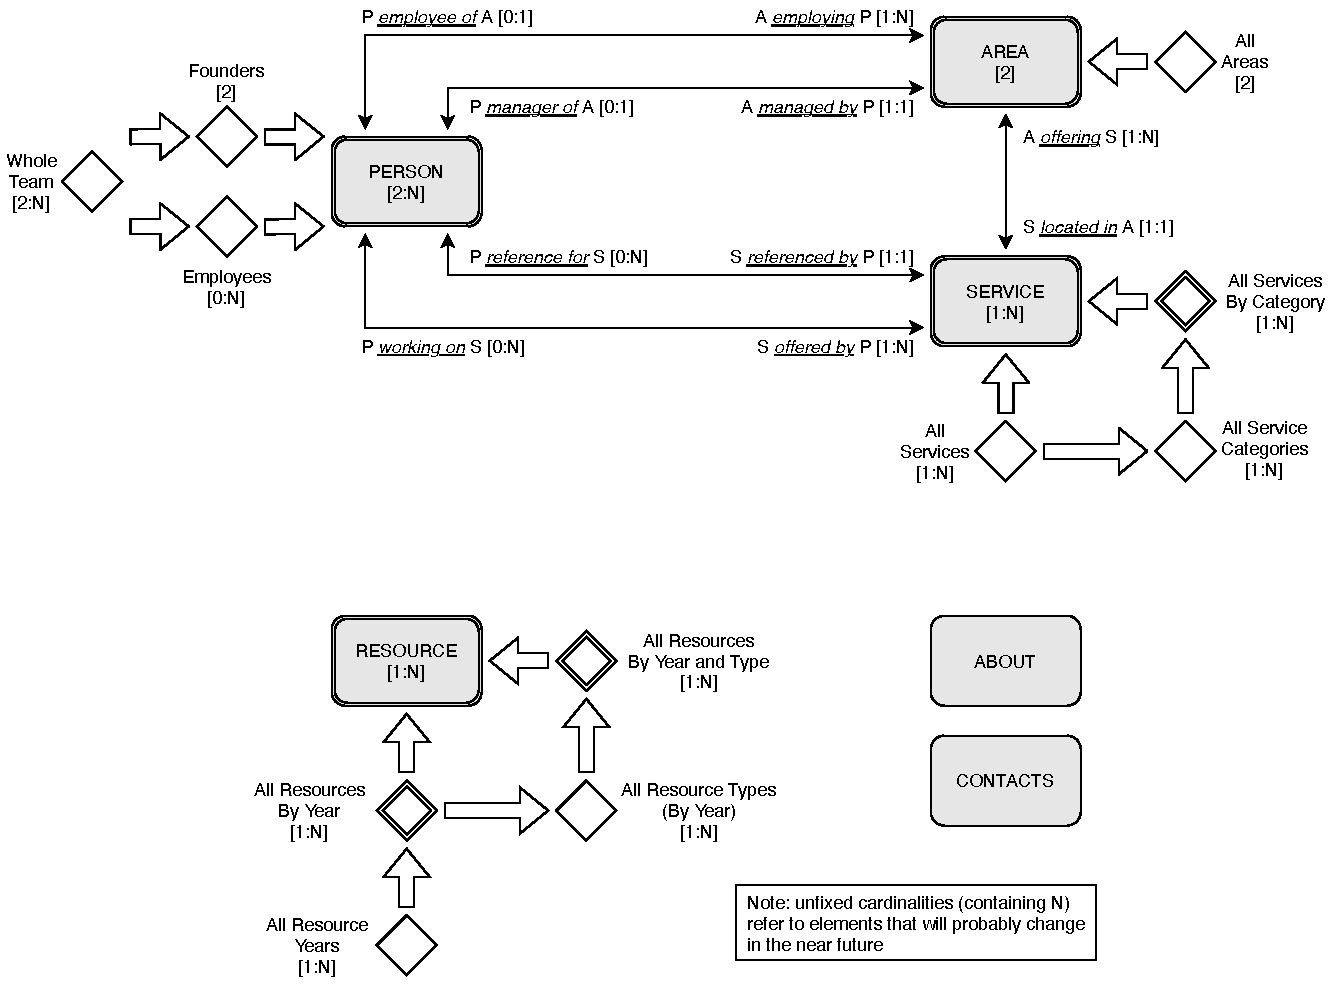
\includegraphics[width=\textwidth]{C-IDM.pdf}
	\caption{C-IDM Diagram}
\end{figure}

\chapter{Content tables}
Here we illustrate the content tables that expand the C-IDM diagram of the previous 
chapter.\\\\
\begin{figure}[h]
	\centering
	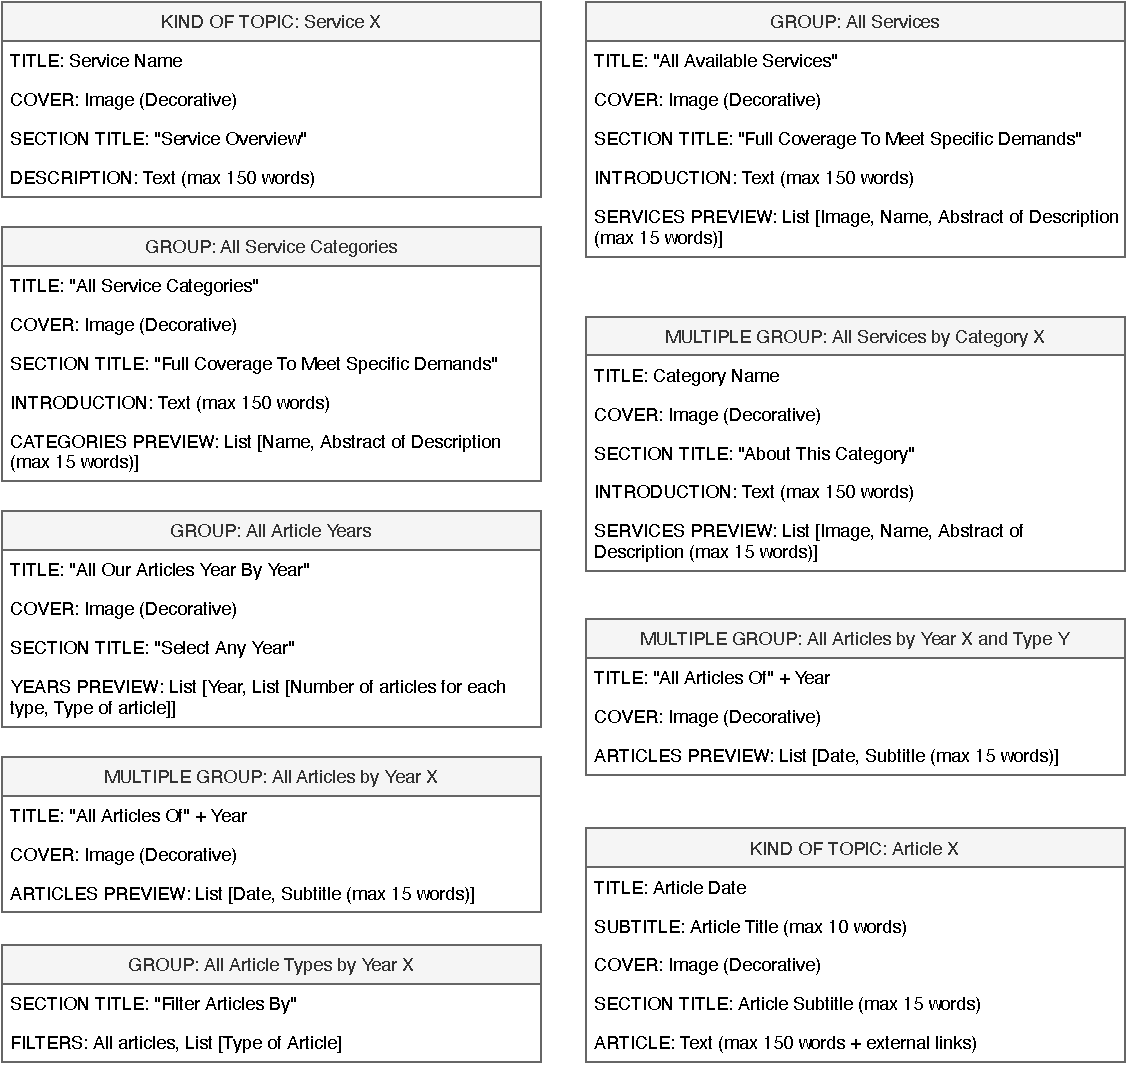
\includegraphics[width=0.9\textwidth]{content_tables_pt2.pdf}
\end{figure}
\begin{figure}[h]
	\centering
	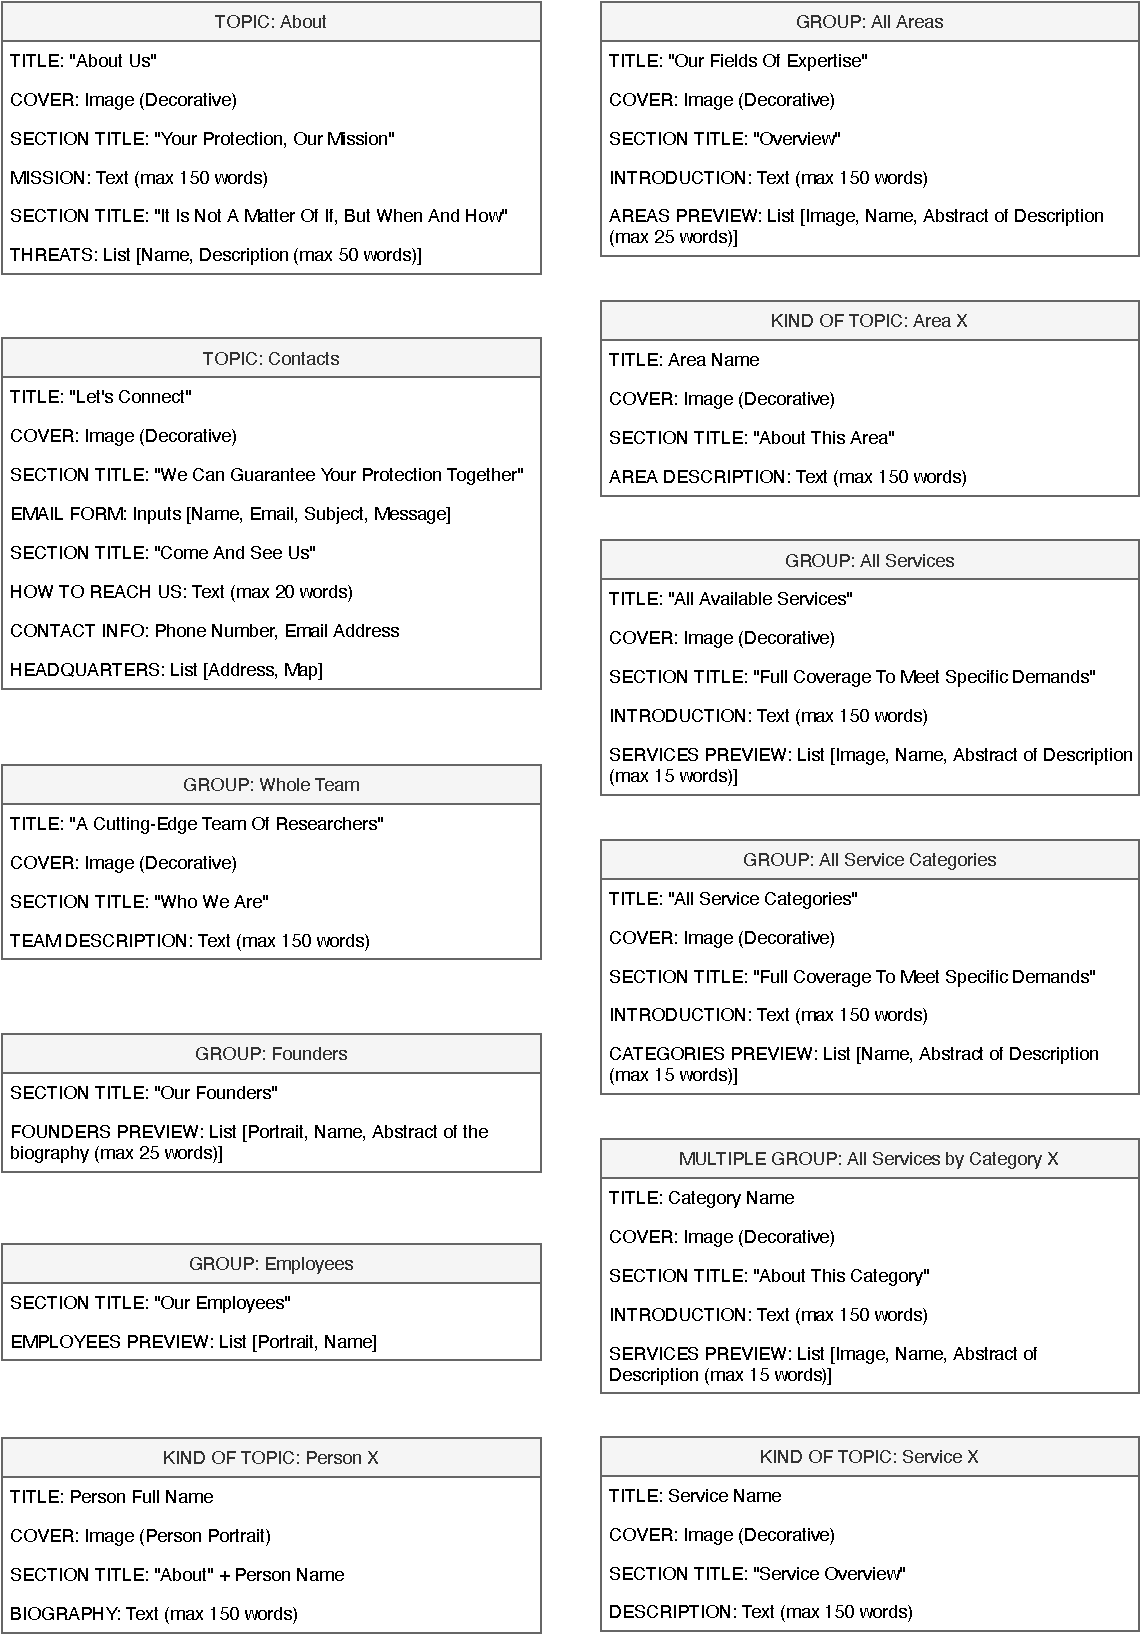
\includegraphics[width=0.9\textwidth]{content_tables_pt1.pdf}
	\caption{Content tables (C-IDM in the small)}
\end{figure}

\chapter{Mapping Content Tables into Pages}
Continuing, we present the result of the application of the process of page mapping 
to the content tables reported in the last chapter. Each table has
been divided into a series of pages, in order to increase the degree of granularity.
\begin{figure}[h]
	\centering
	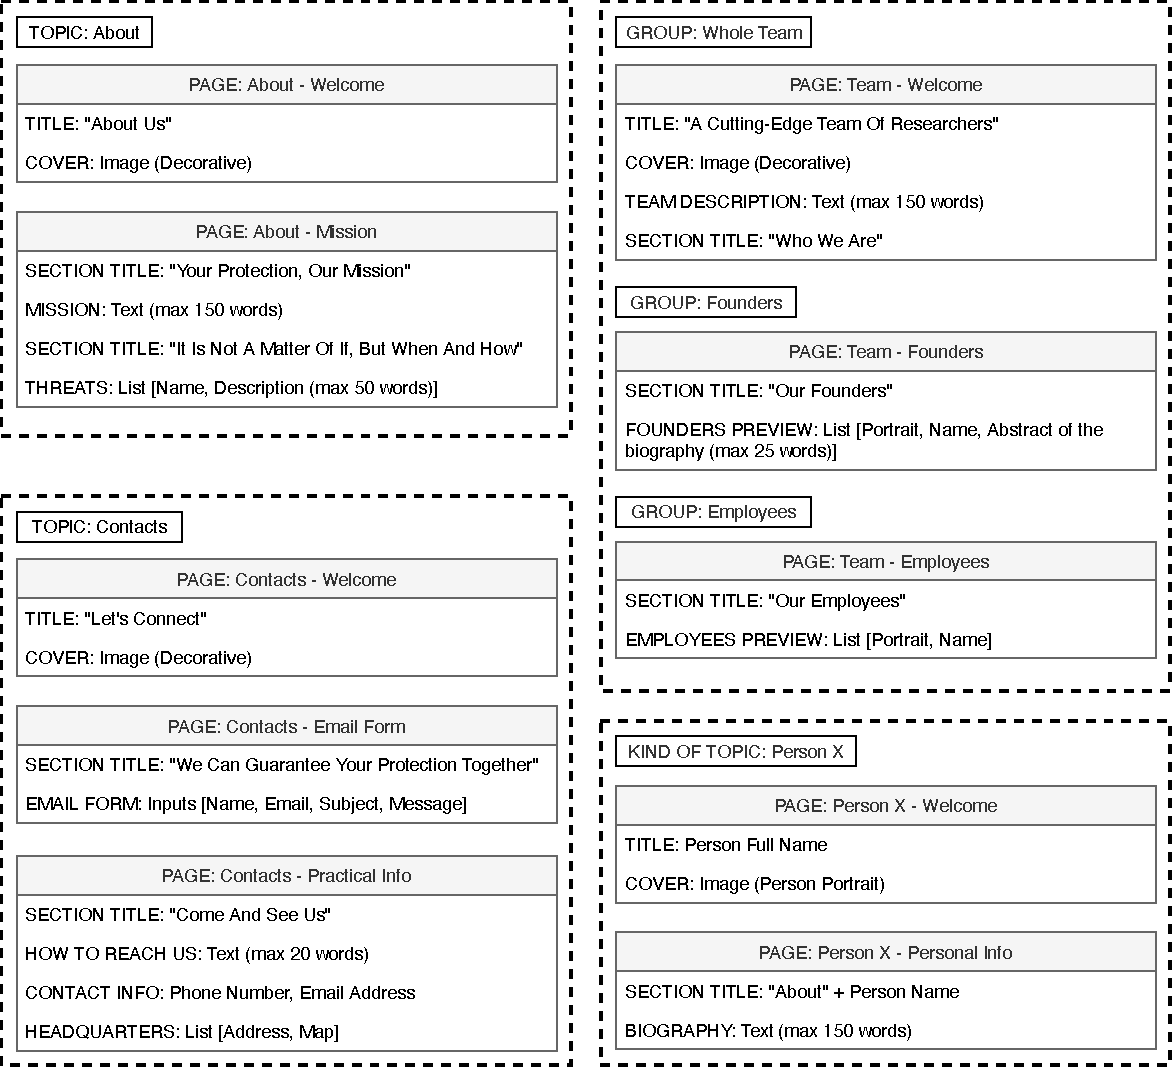
\includegraphics[width=0.95\textwidth]{page_mapping_pt1.pdf}
\end{figure}
\begin{figure}[h]
	\centering
	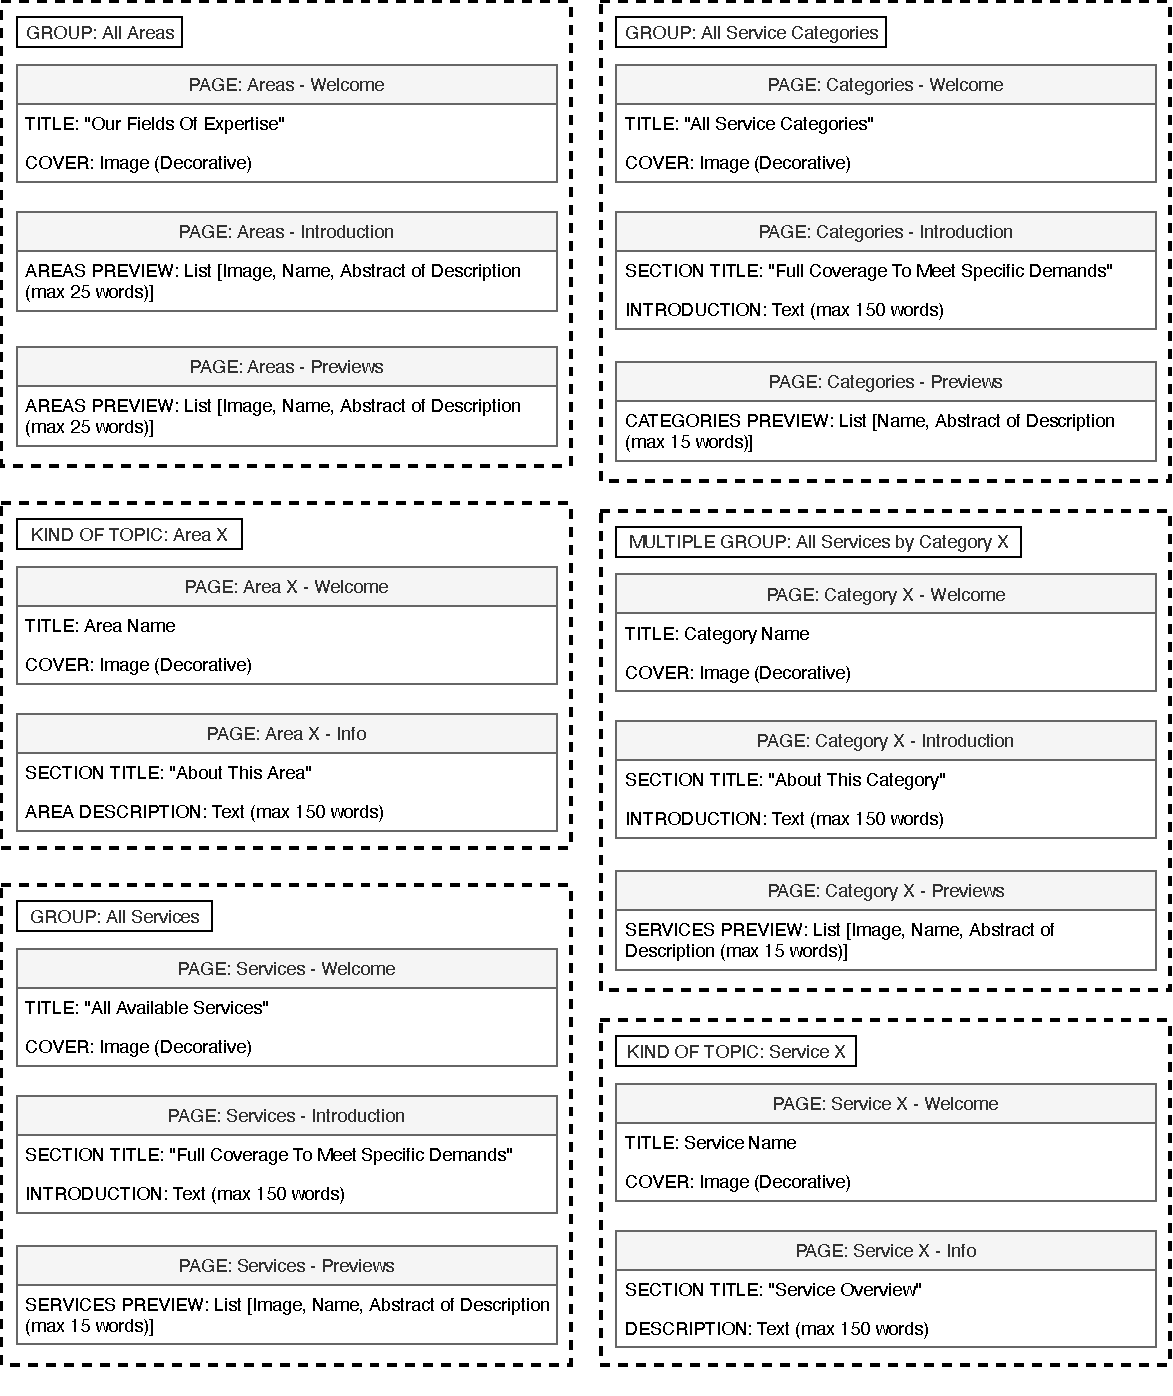
\includegraphics[width=0.95\textwidth]{page_mapping_pt2.pdf}
\end{figure}
\begin{figure}[h]
	\centering
	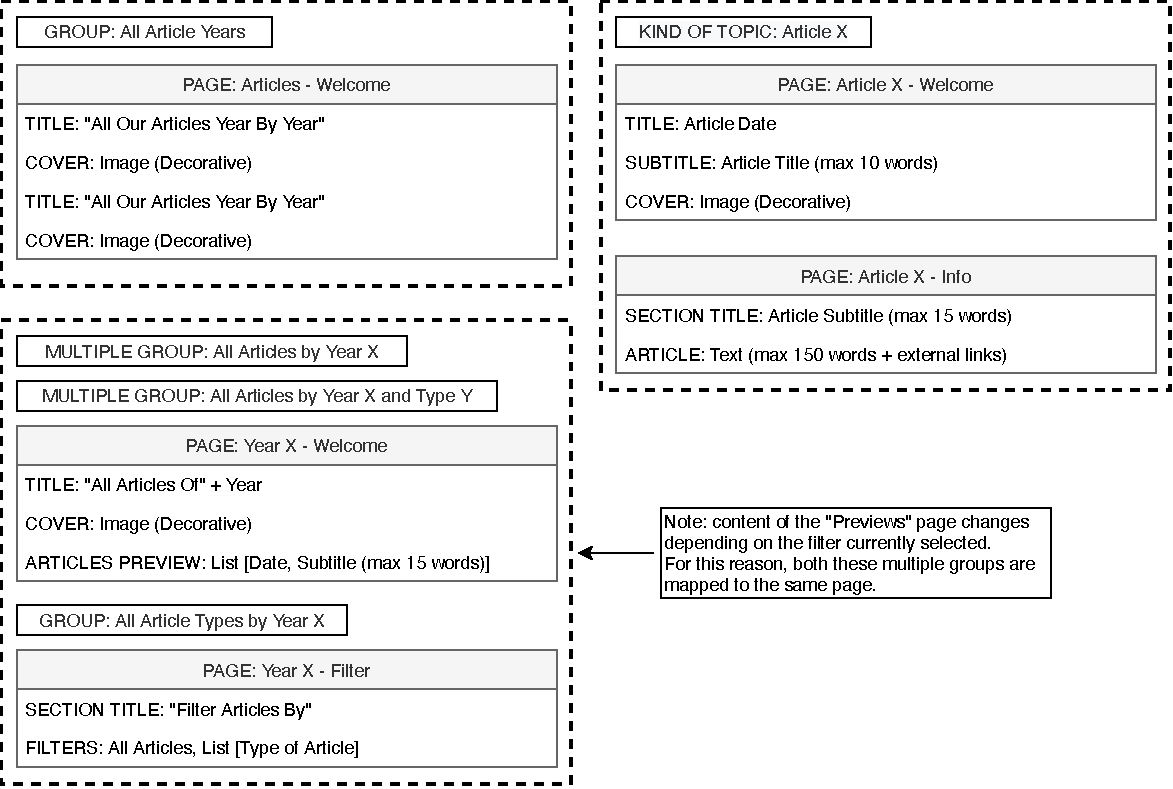
\includegraphics[width=0.95\textwidth]{page_mapping_pt3.pdf}
	\caption{Pages mapping}
\end{figure}

\chapter{P-IDM diagram}
In this section we report the P-IDM diagram which describes the navigation design of our website.\\
\begin{figure}[h]
	\centering
	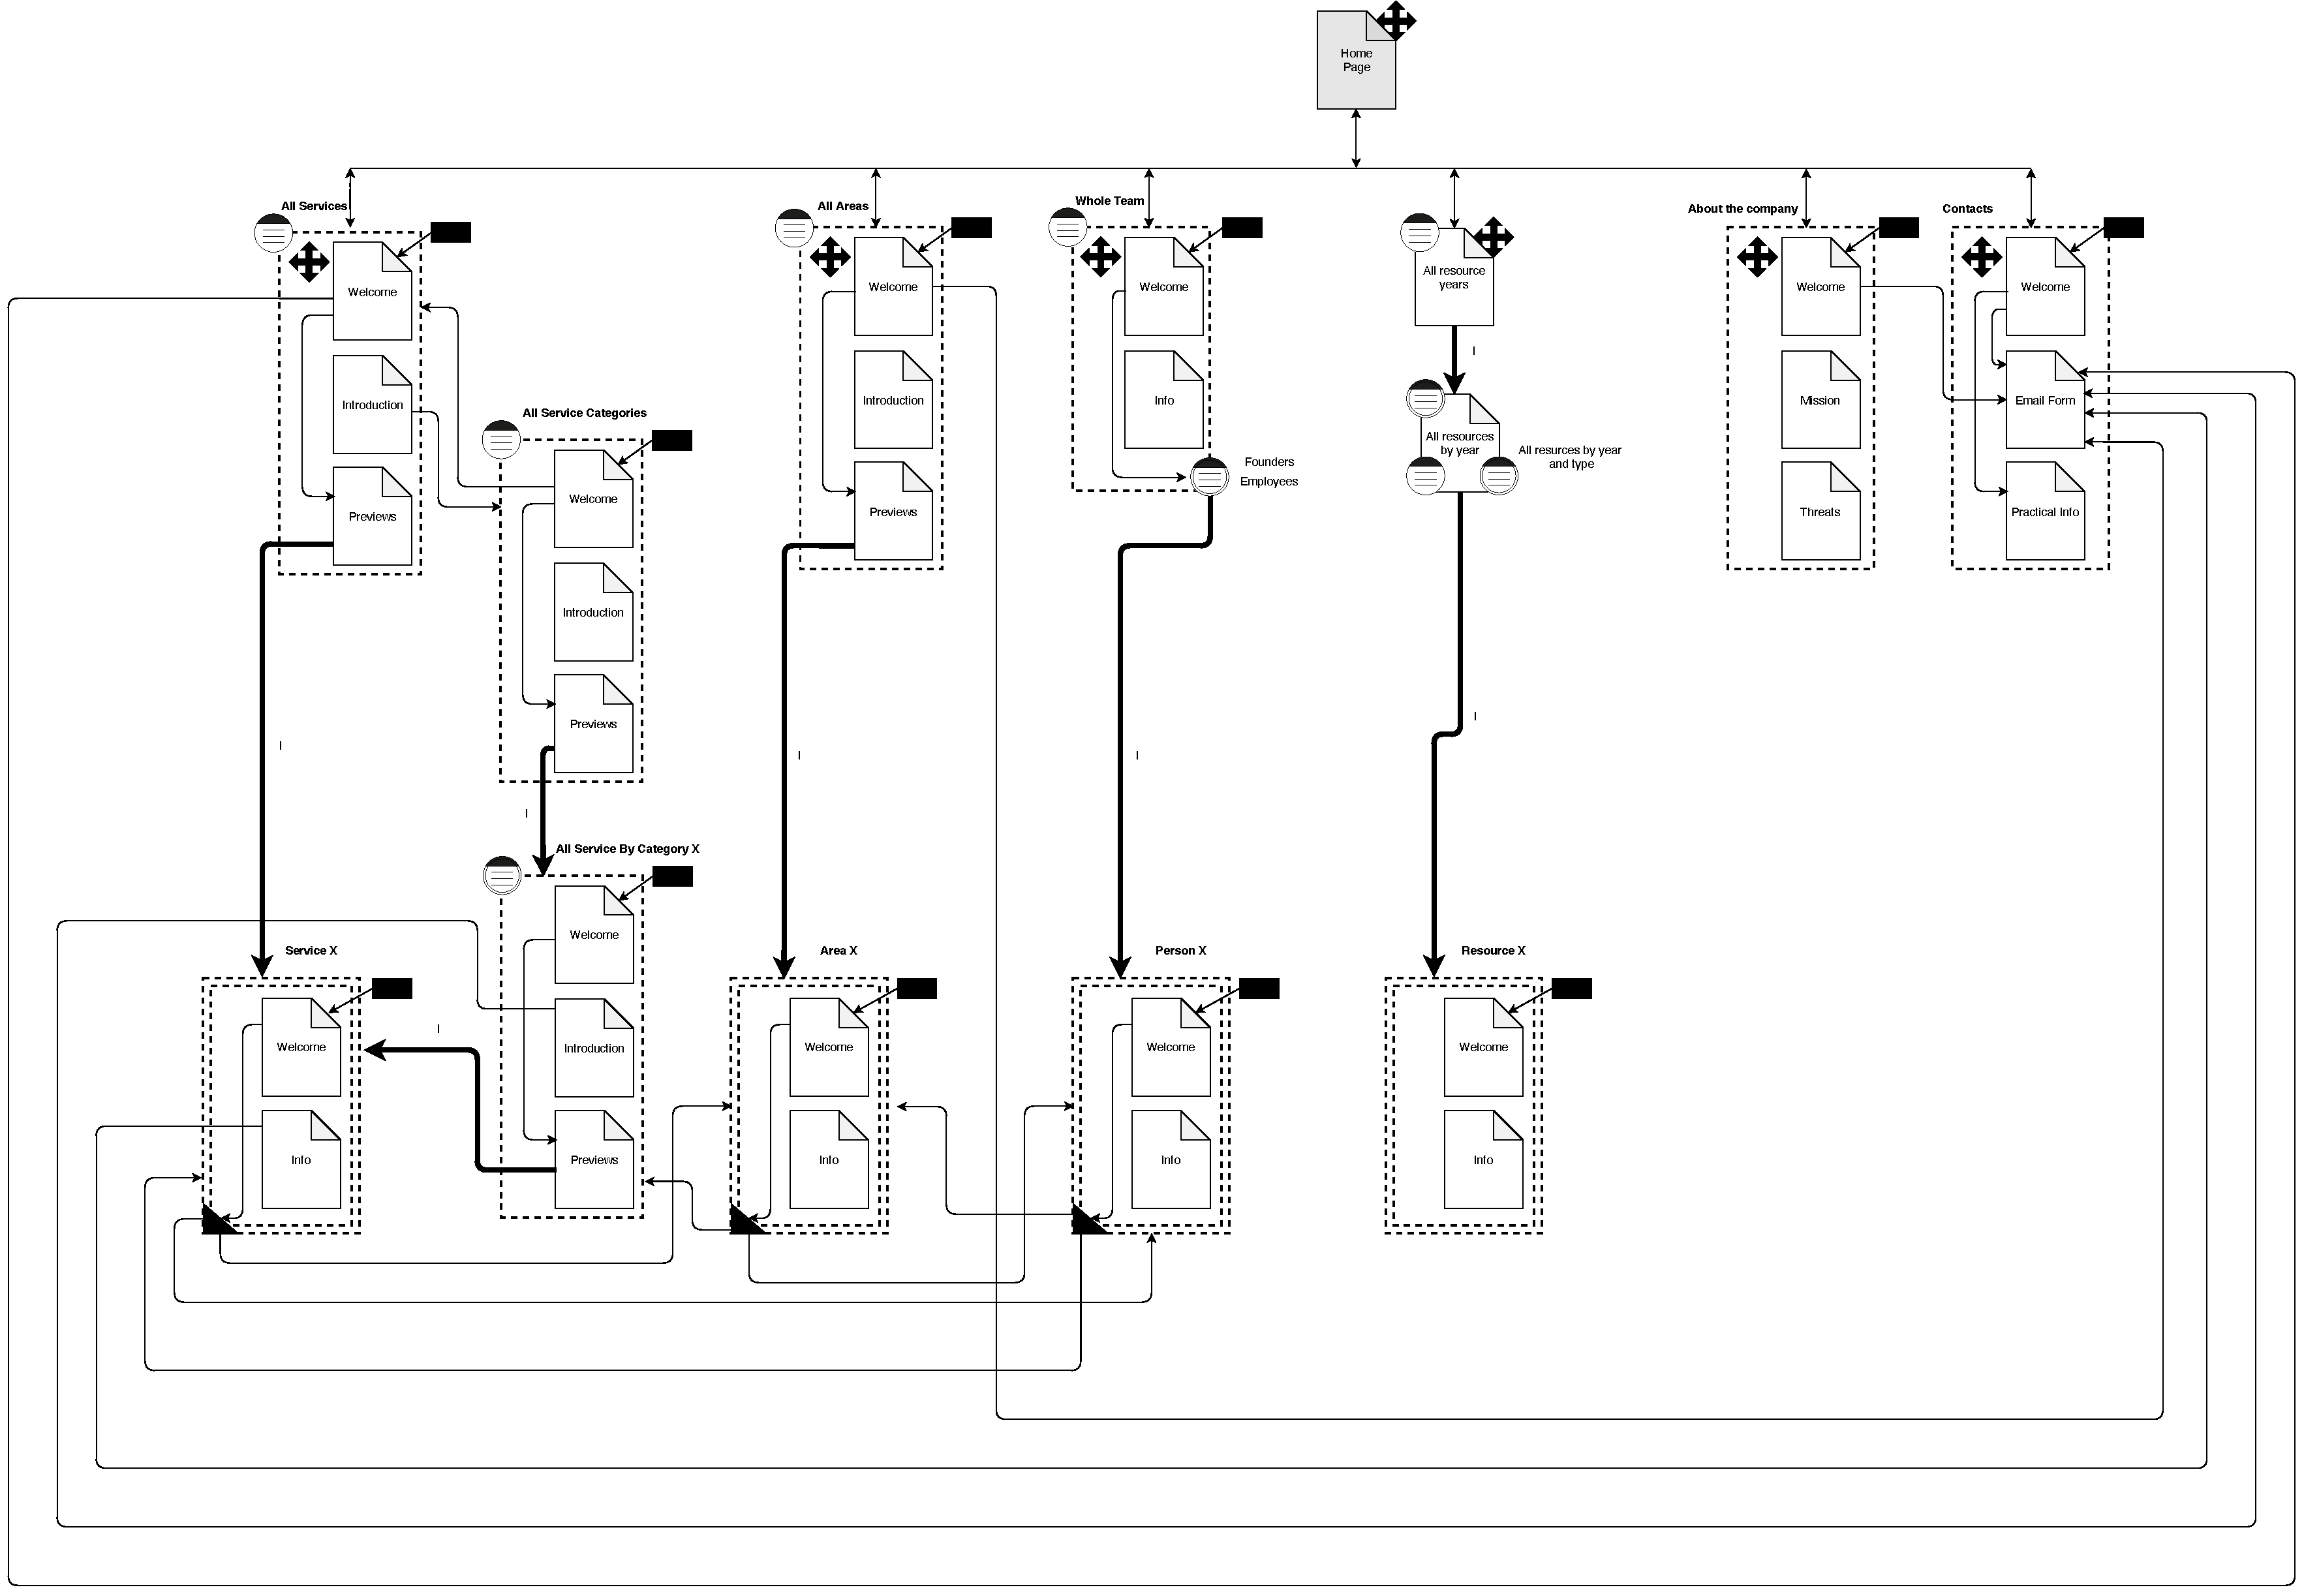
\includegraphics[width=\textwidth]{P-IDM.pdf}
	\caption{P-IDM Diagram}
\end{figure}

\chapter{Visual Design}

\section{Low-Fidelity Wireframes}

\subsection{Home Page}

\begin{figure}[H]
	\centering
	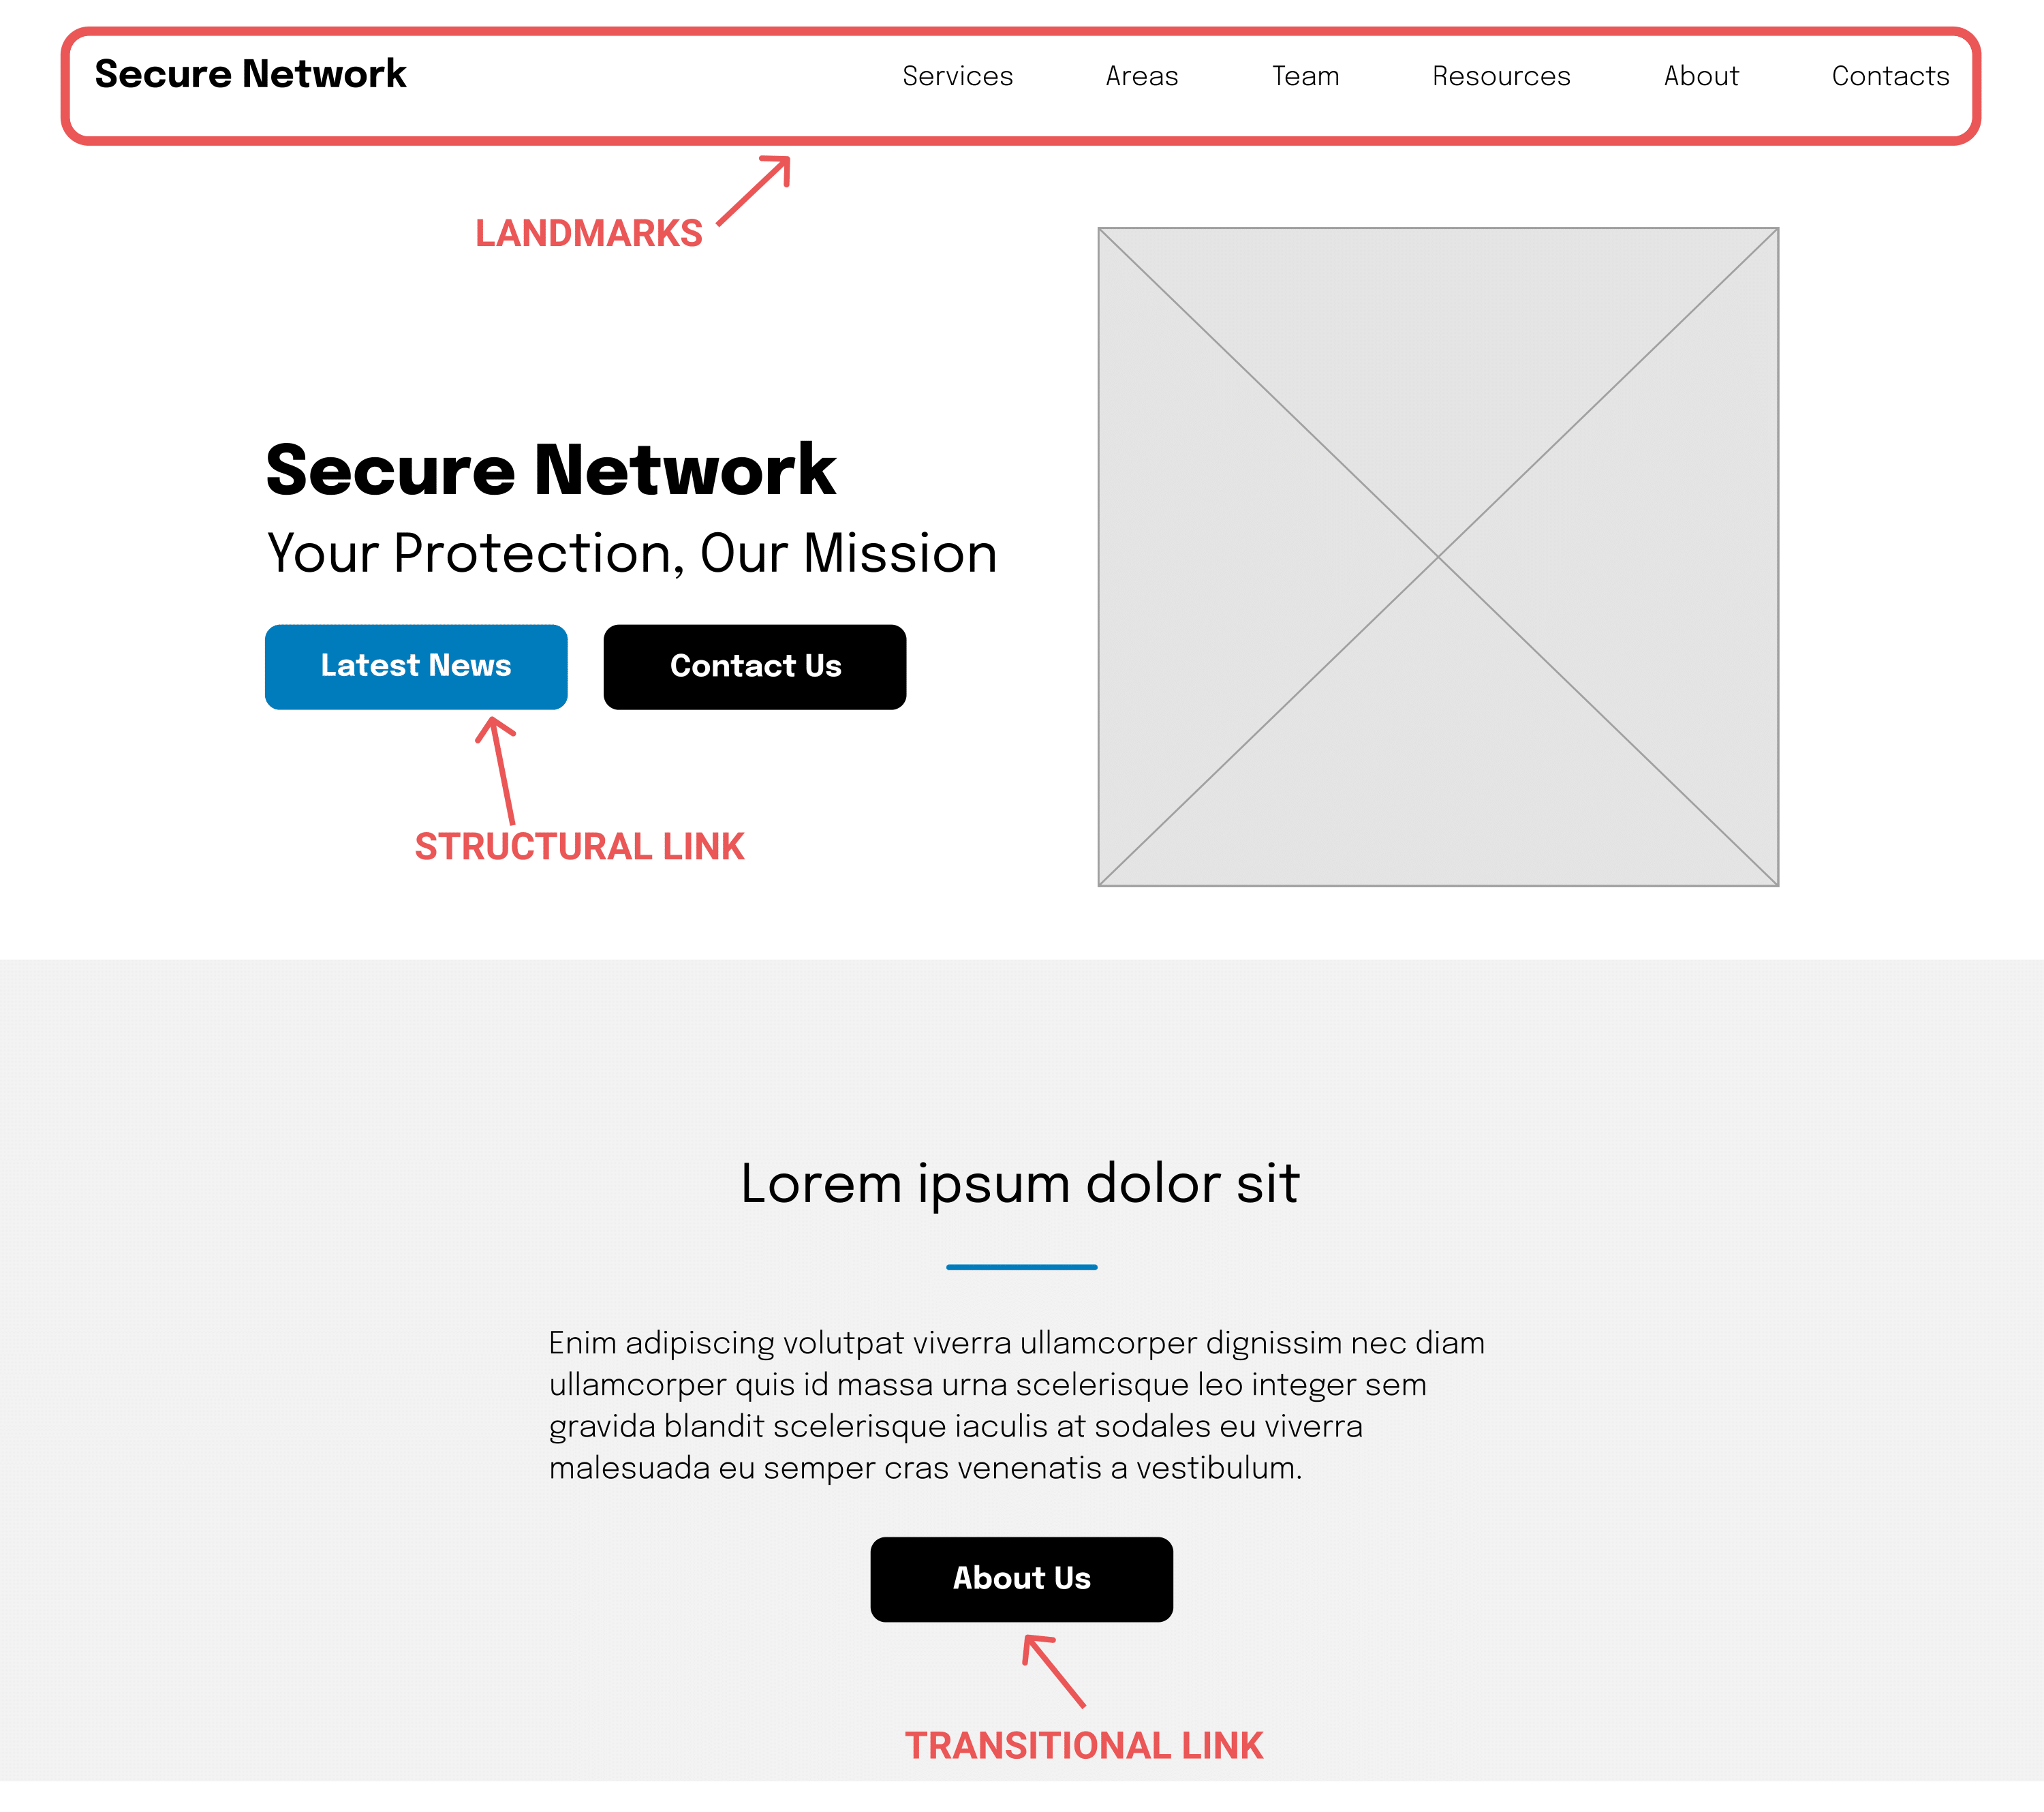
\includegraphics[width=0.45\textwidth]{low_fid_wireframes/home/1.png}
	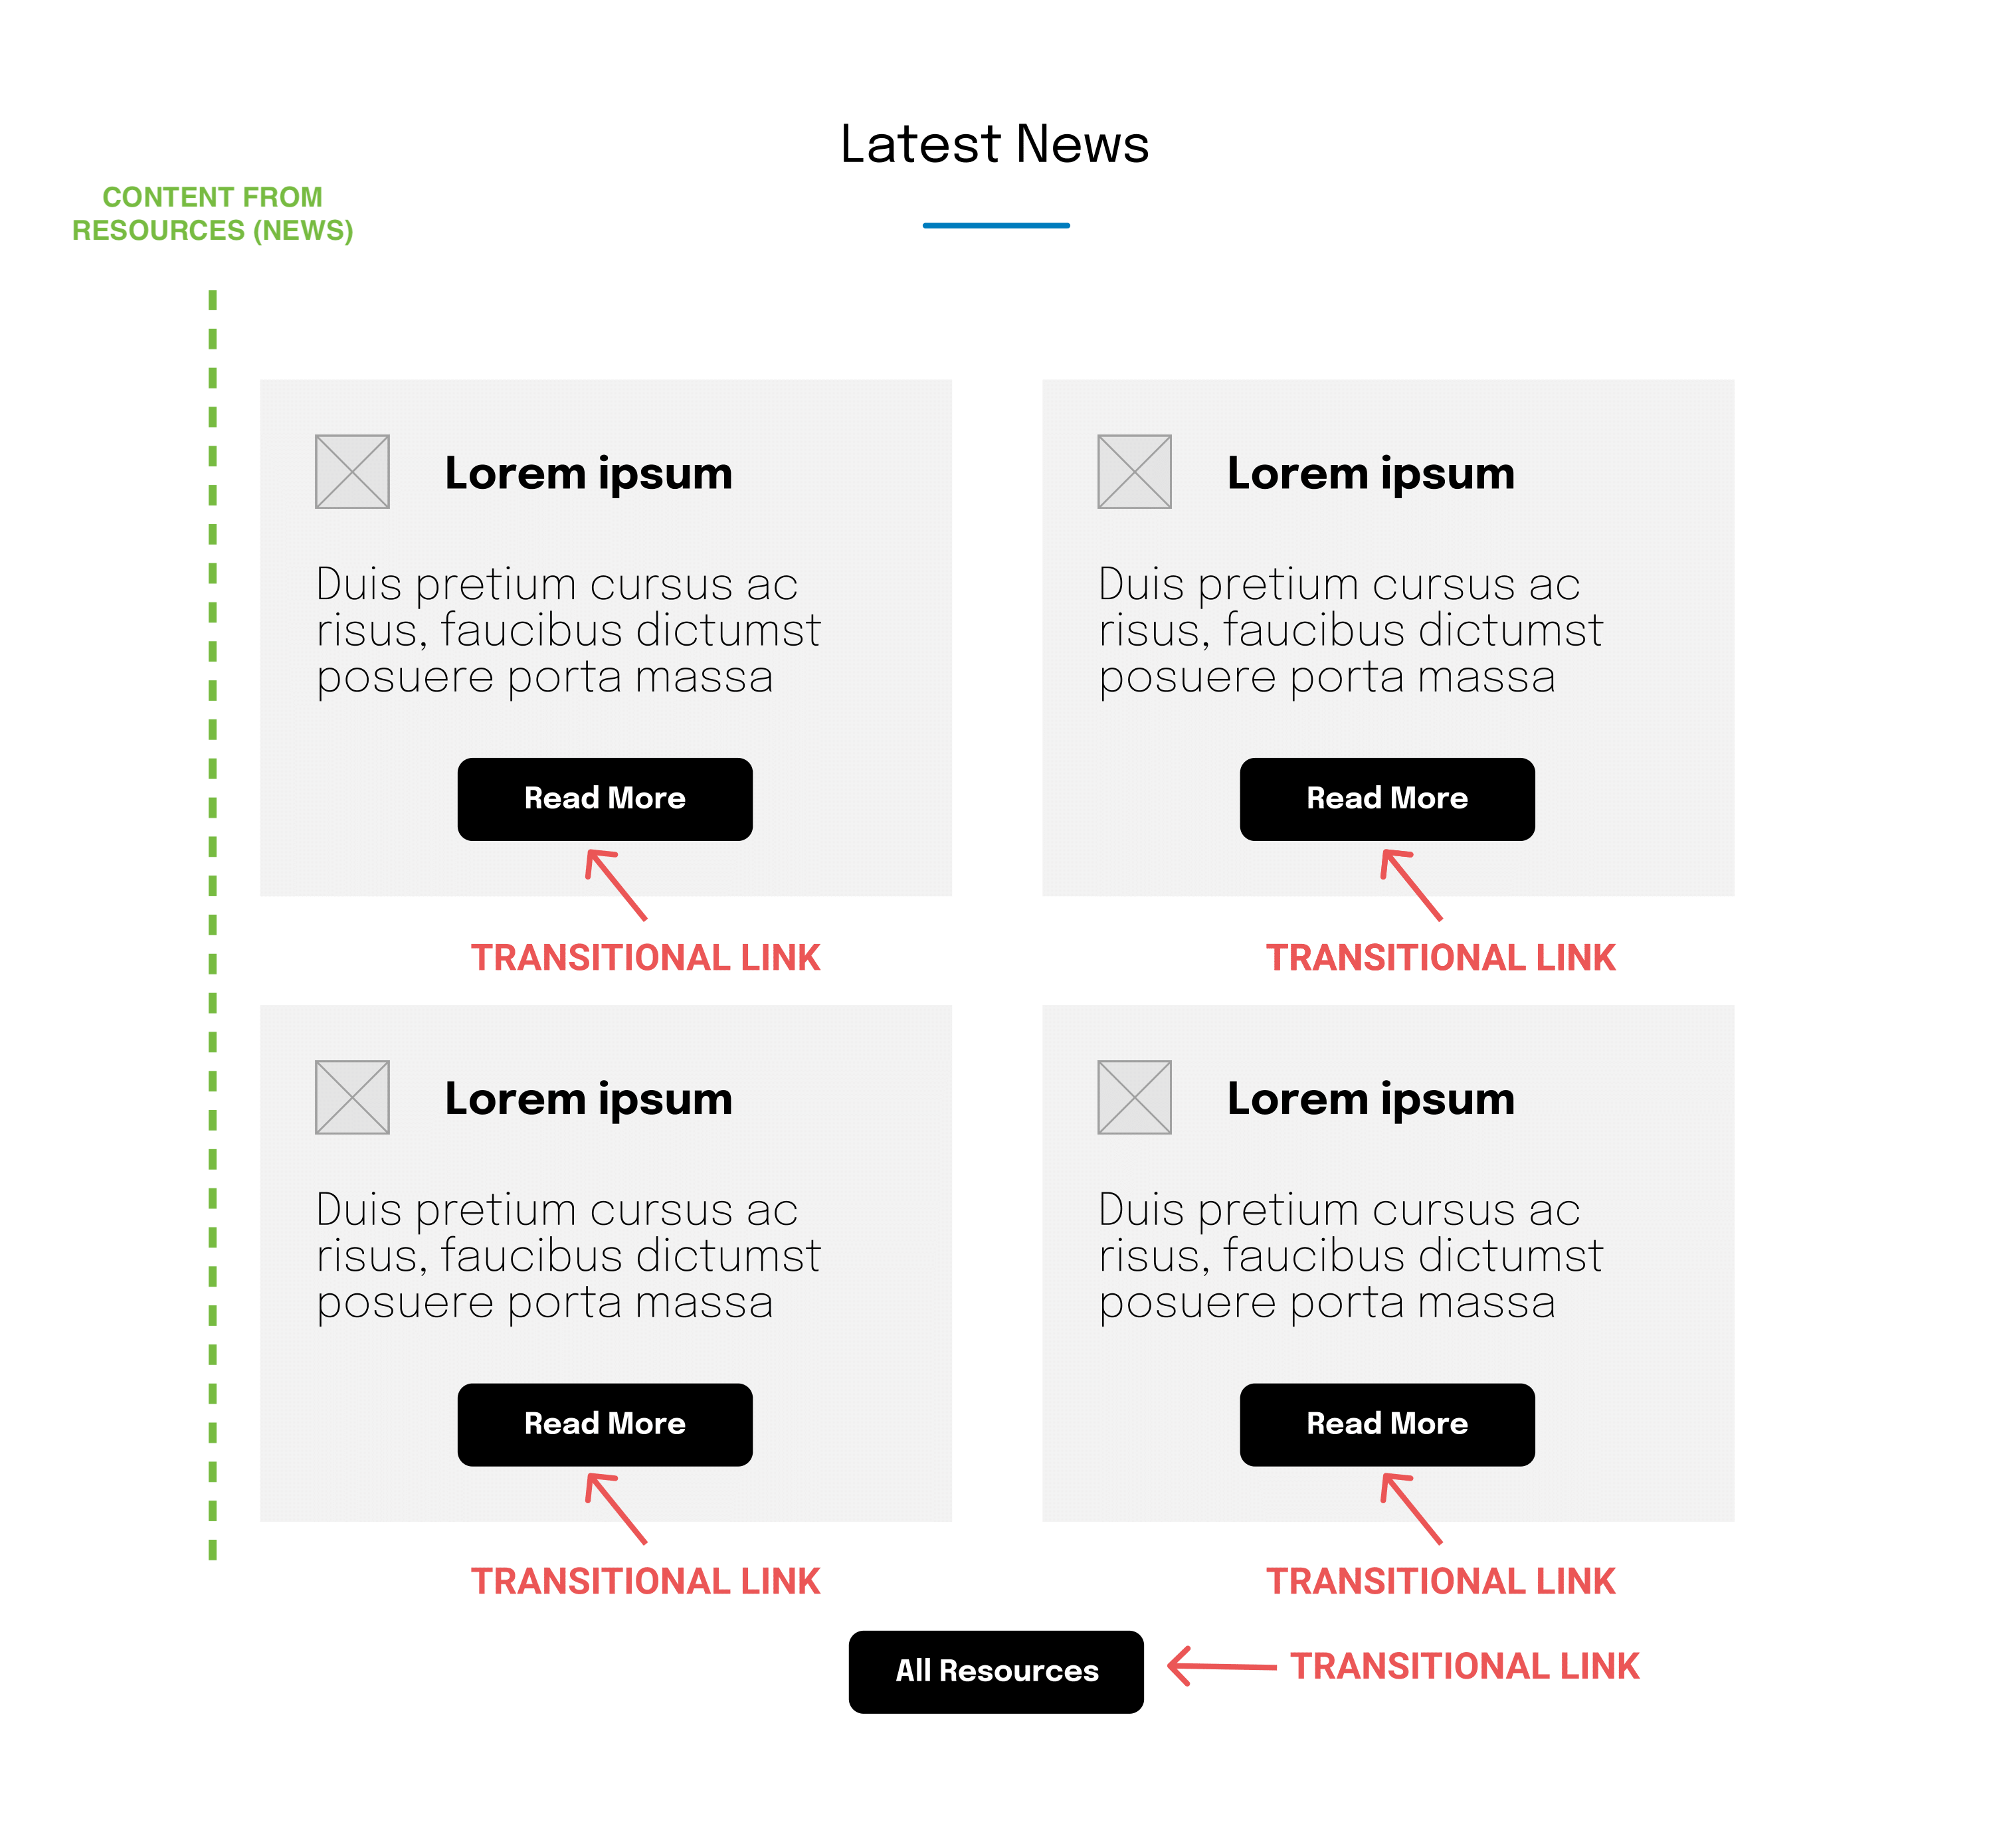
\includegraphics[width=0.45\textwidth]{low_fid_wireframes/home/2.png}
	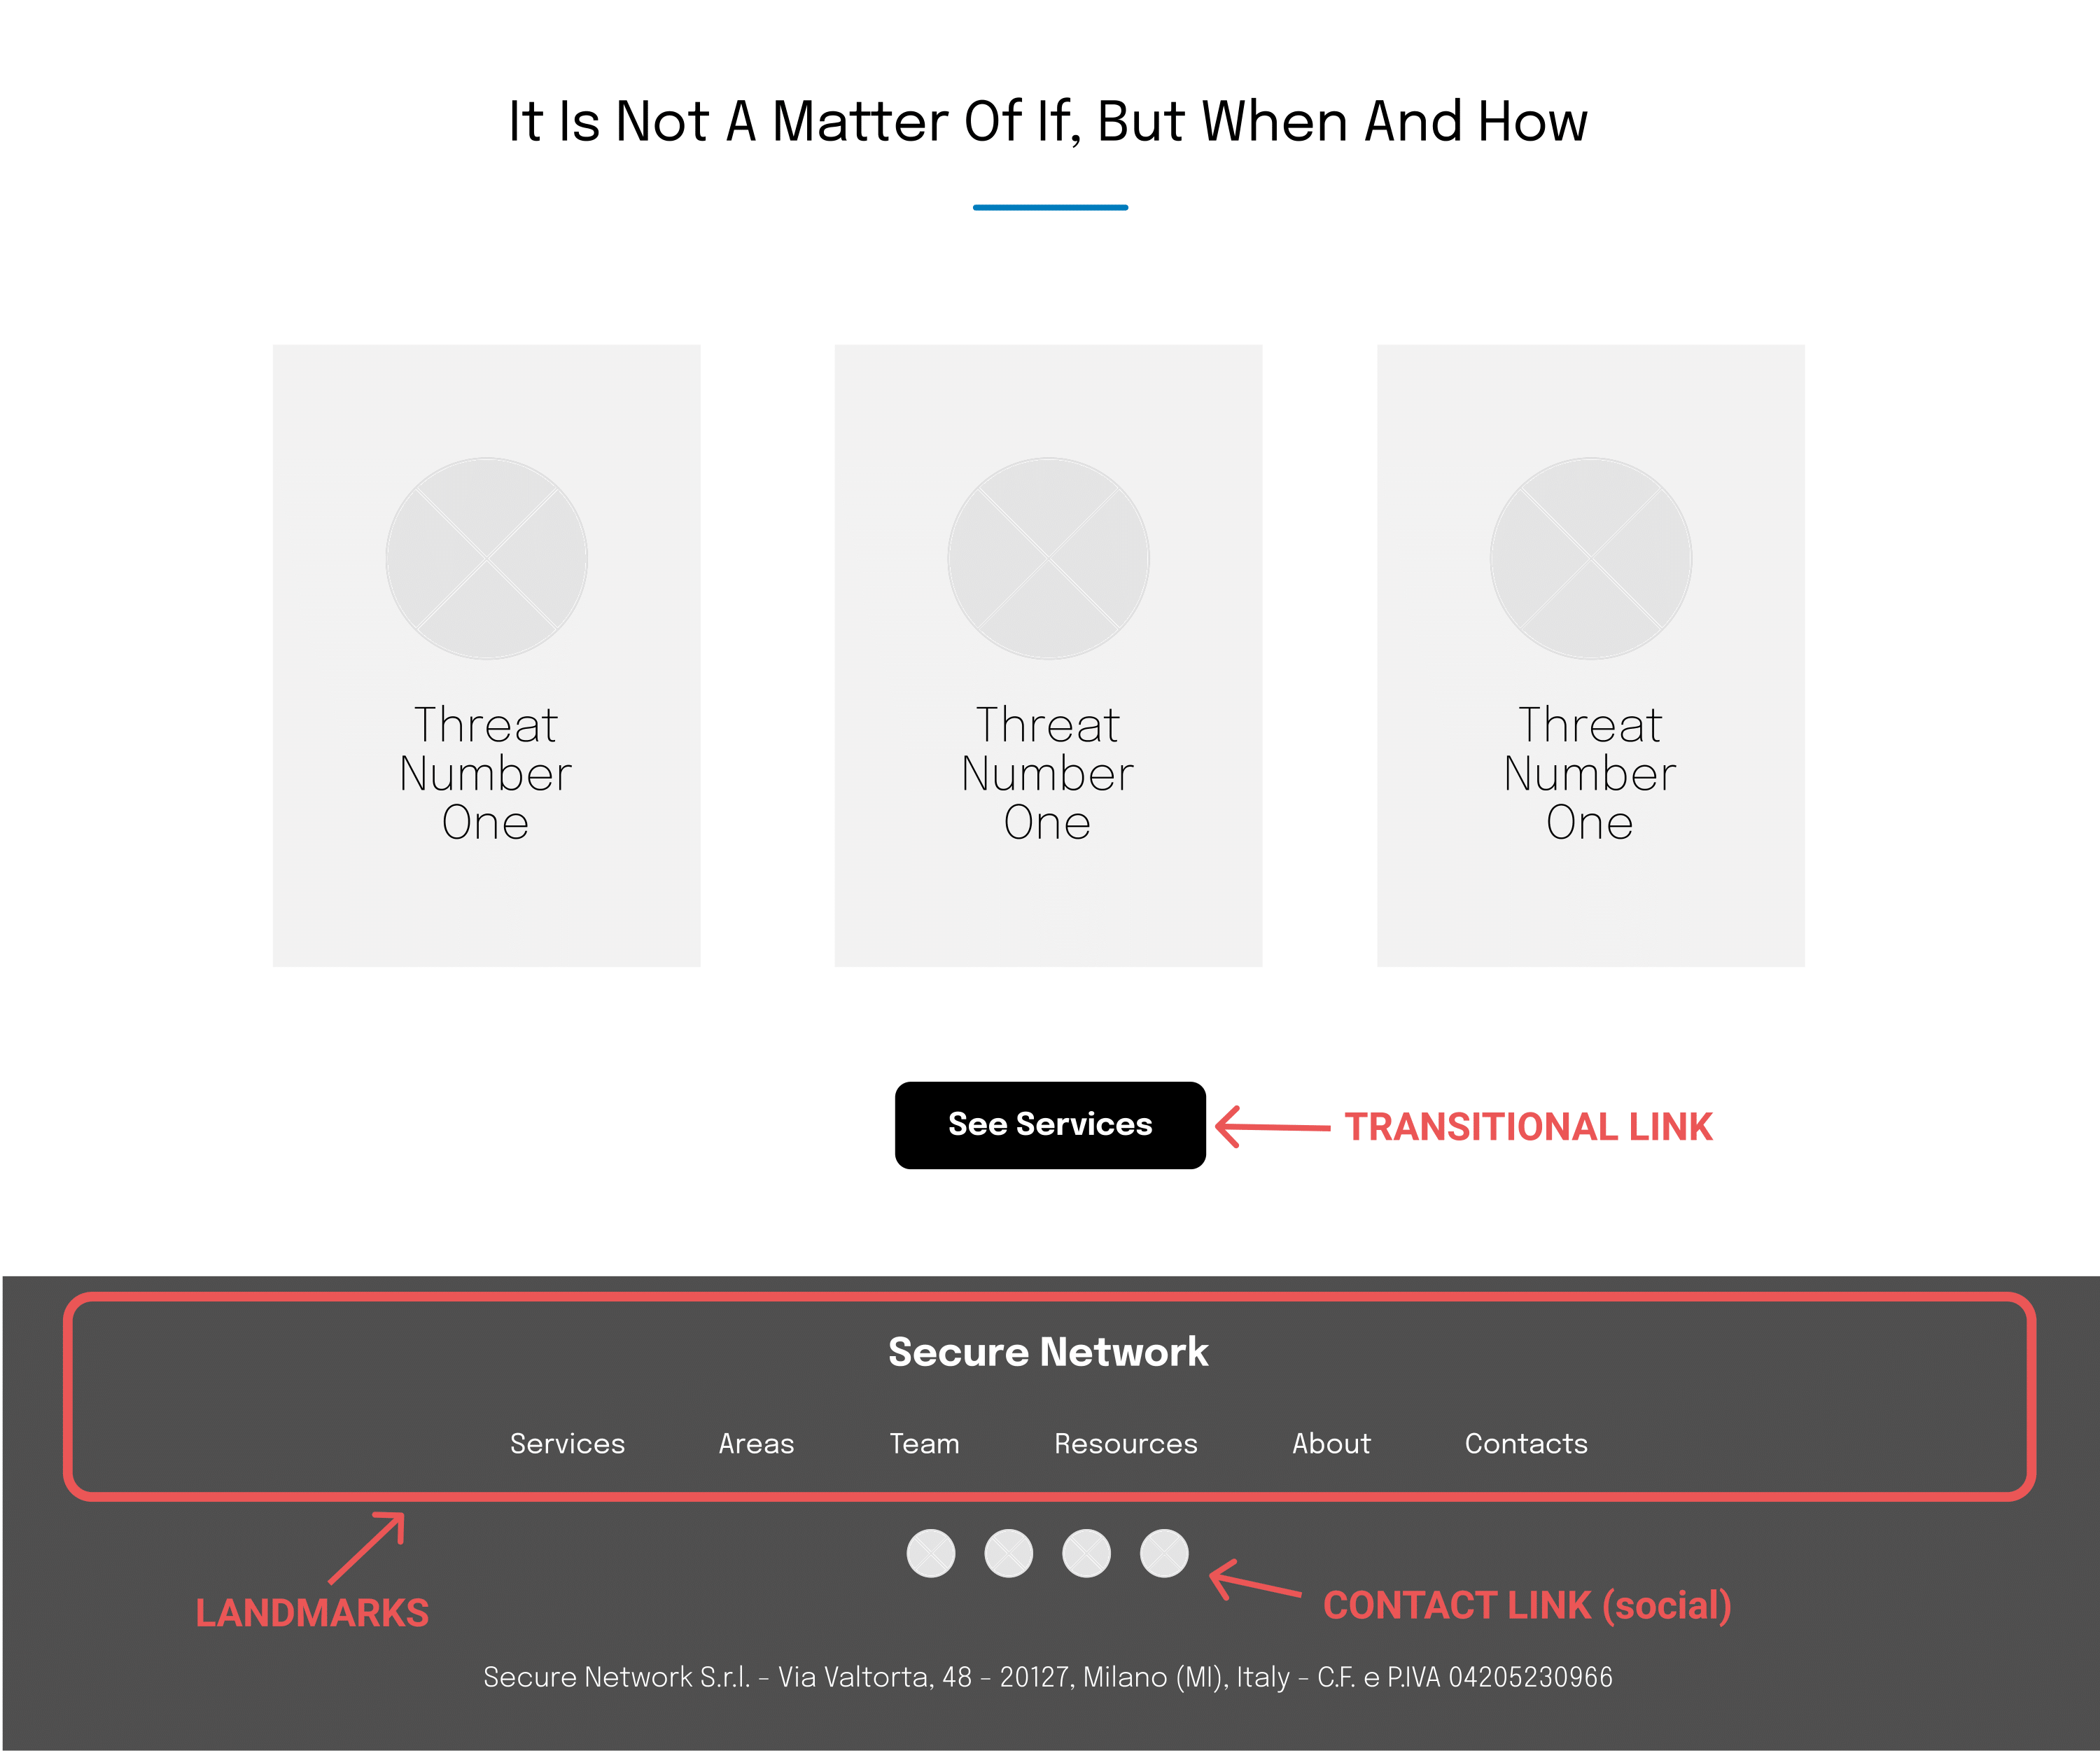
\includegraphics[width=0.45\textwidth]{low_fid_wireframes/home/3.png}
	\caption{Commented wireframes for the Home page.}
\end{figure}

\subsection{Topic: Contacts}

\begin{figure}[H]
	\centering
	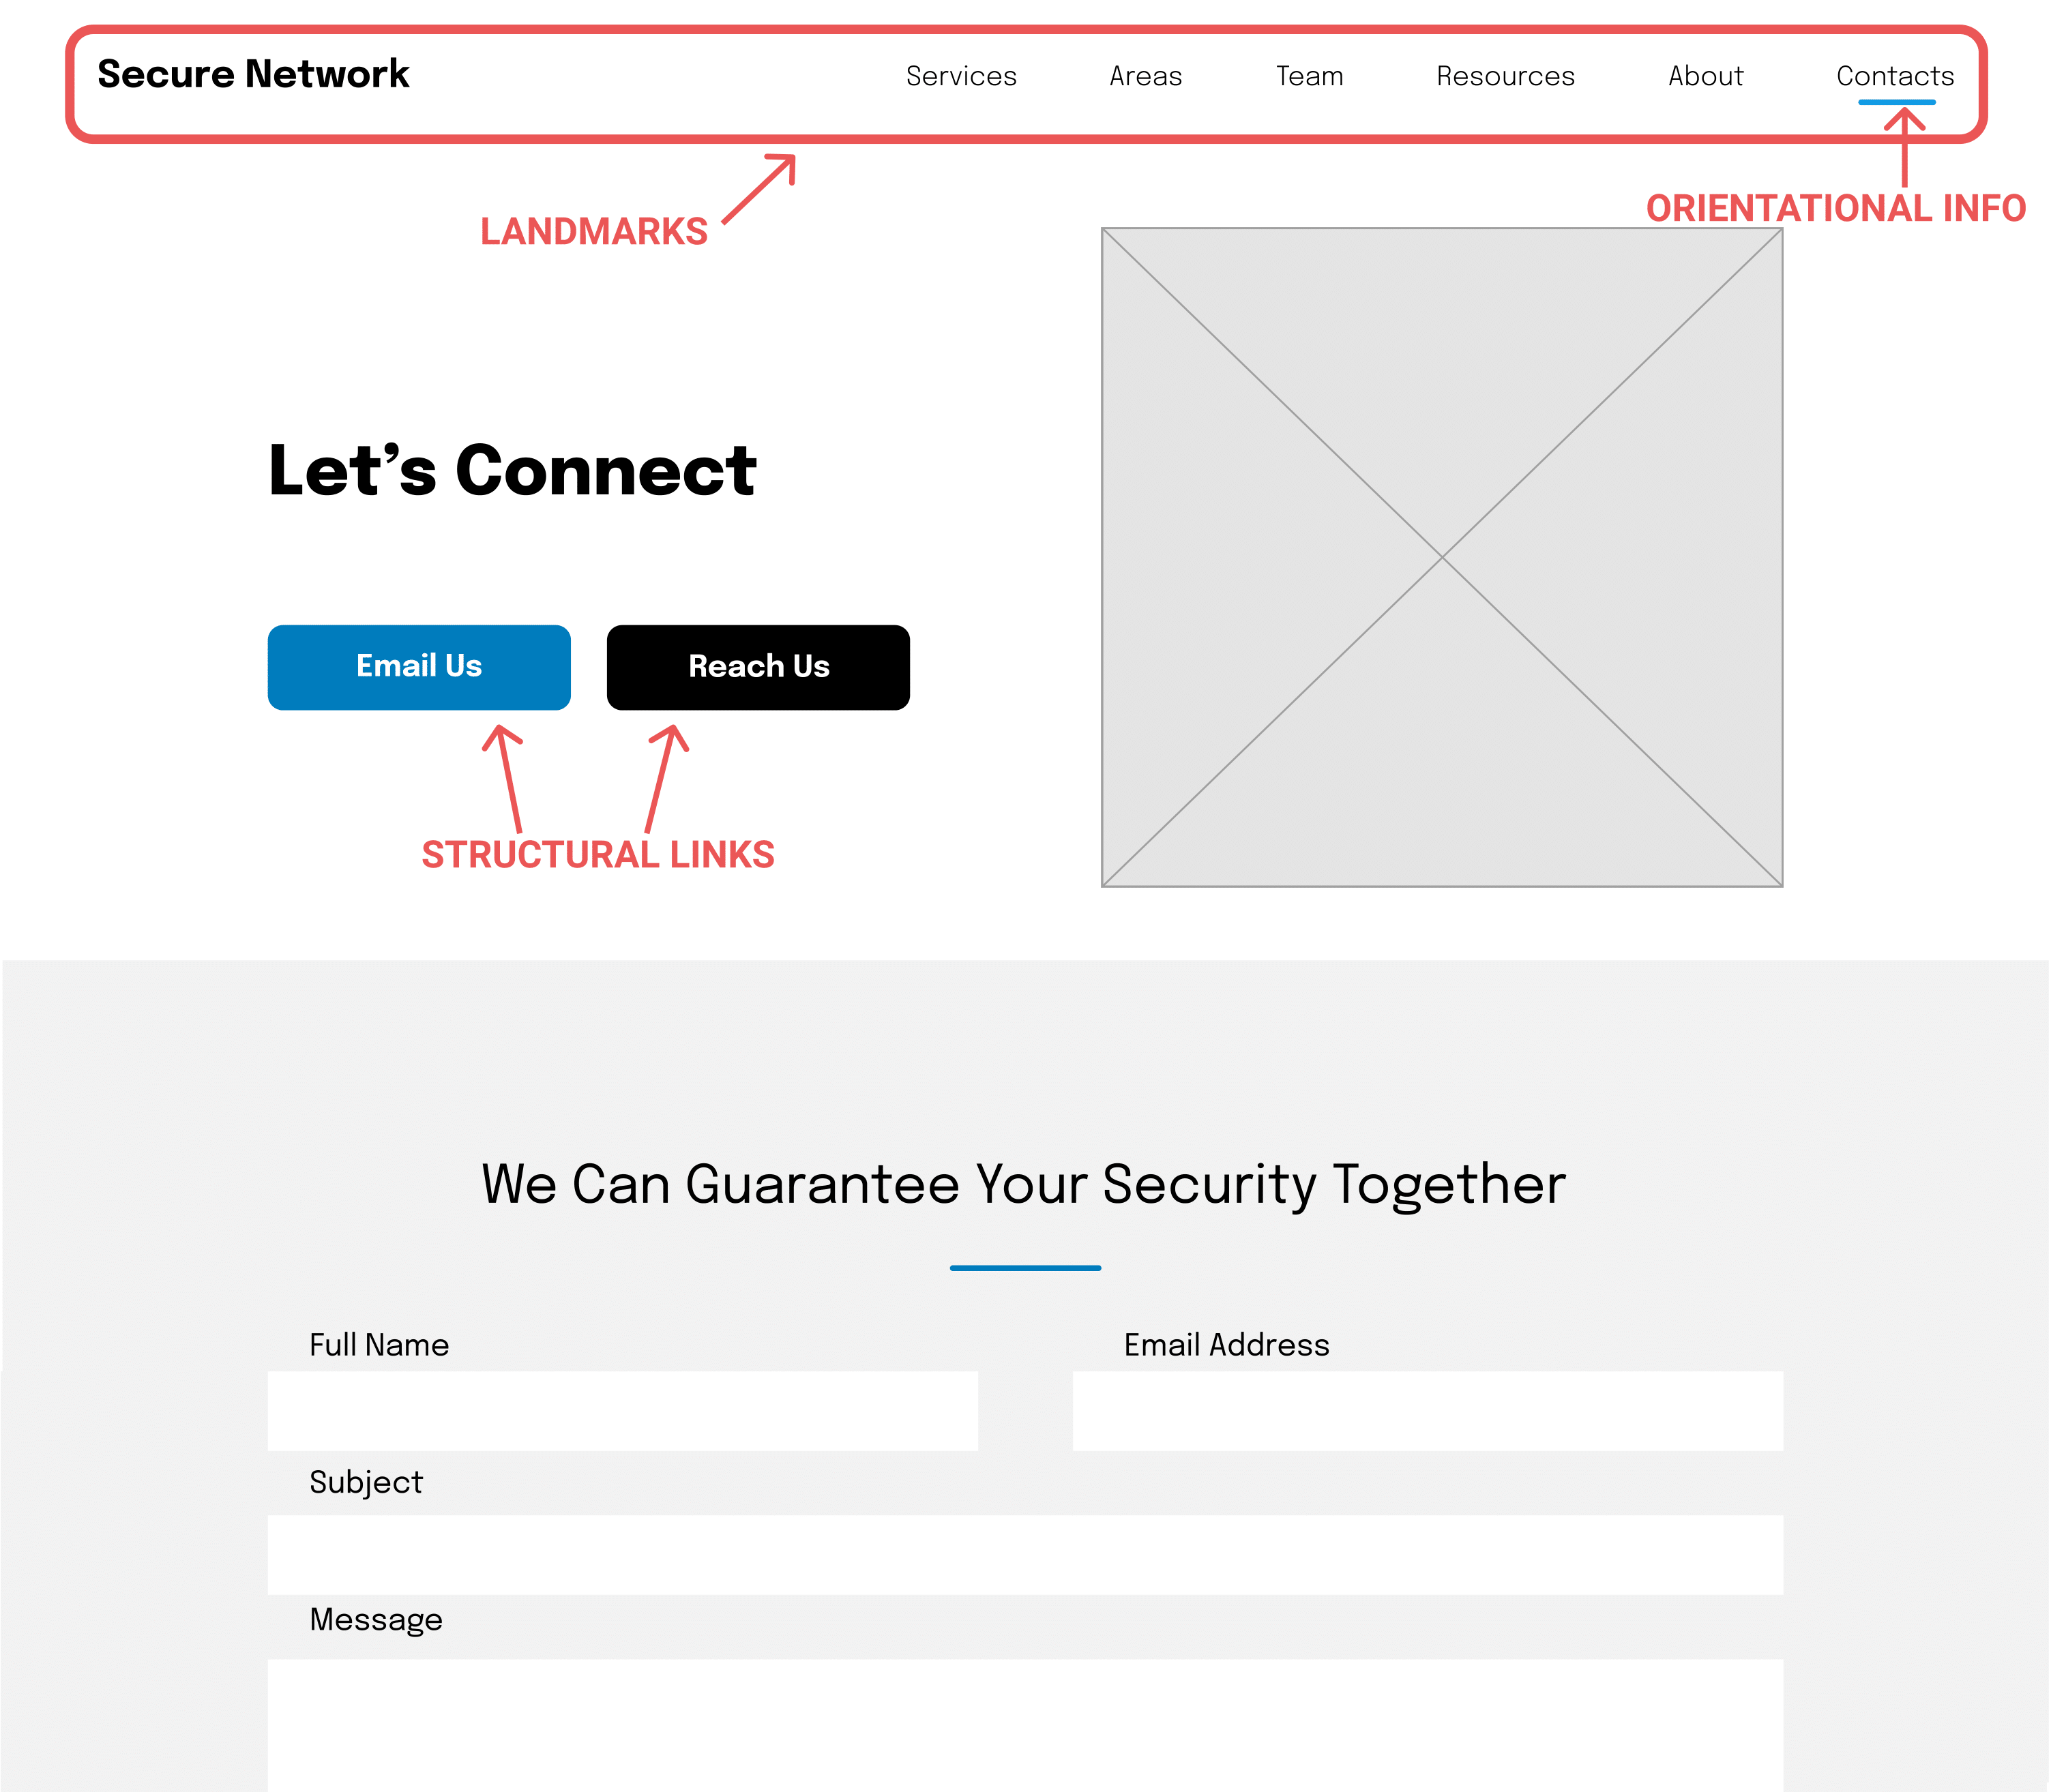
\includegraphics[width=0.45\textwidth]{low_fid_wireframes/contacts/1.png}
	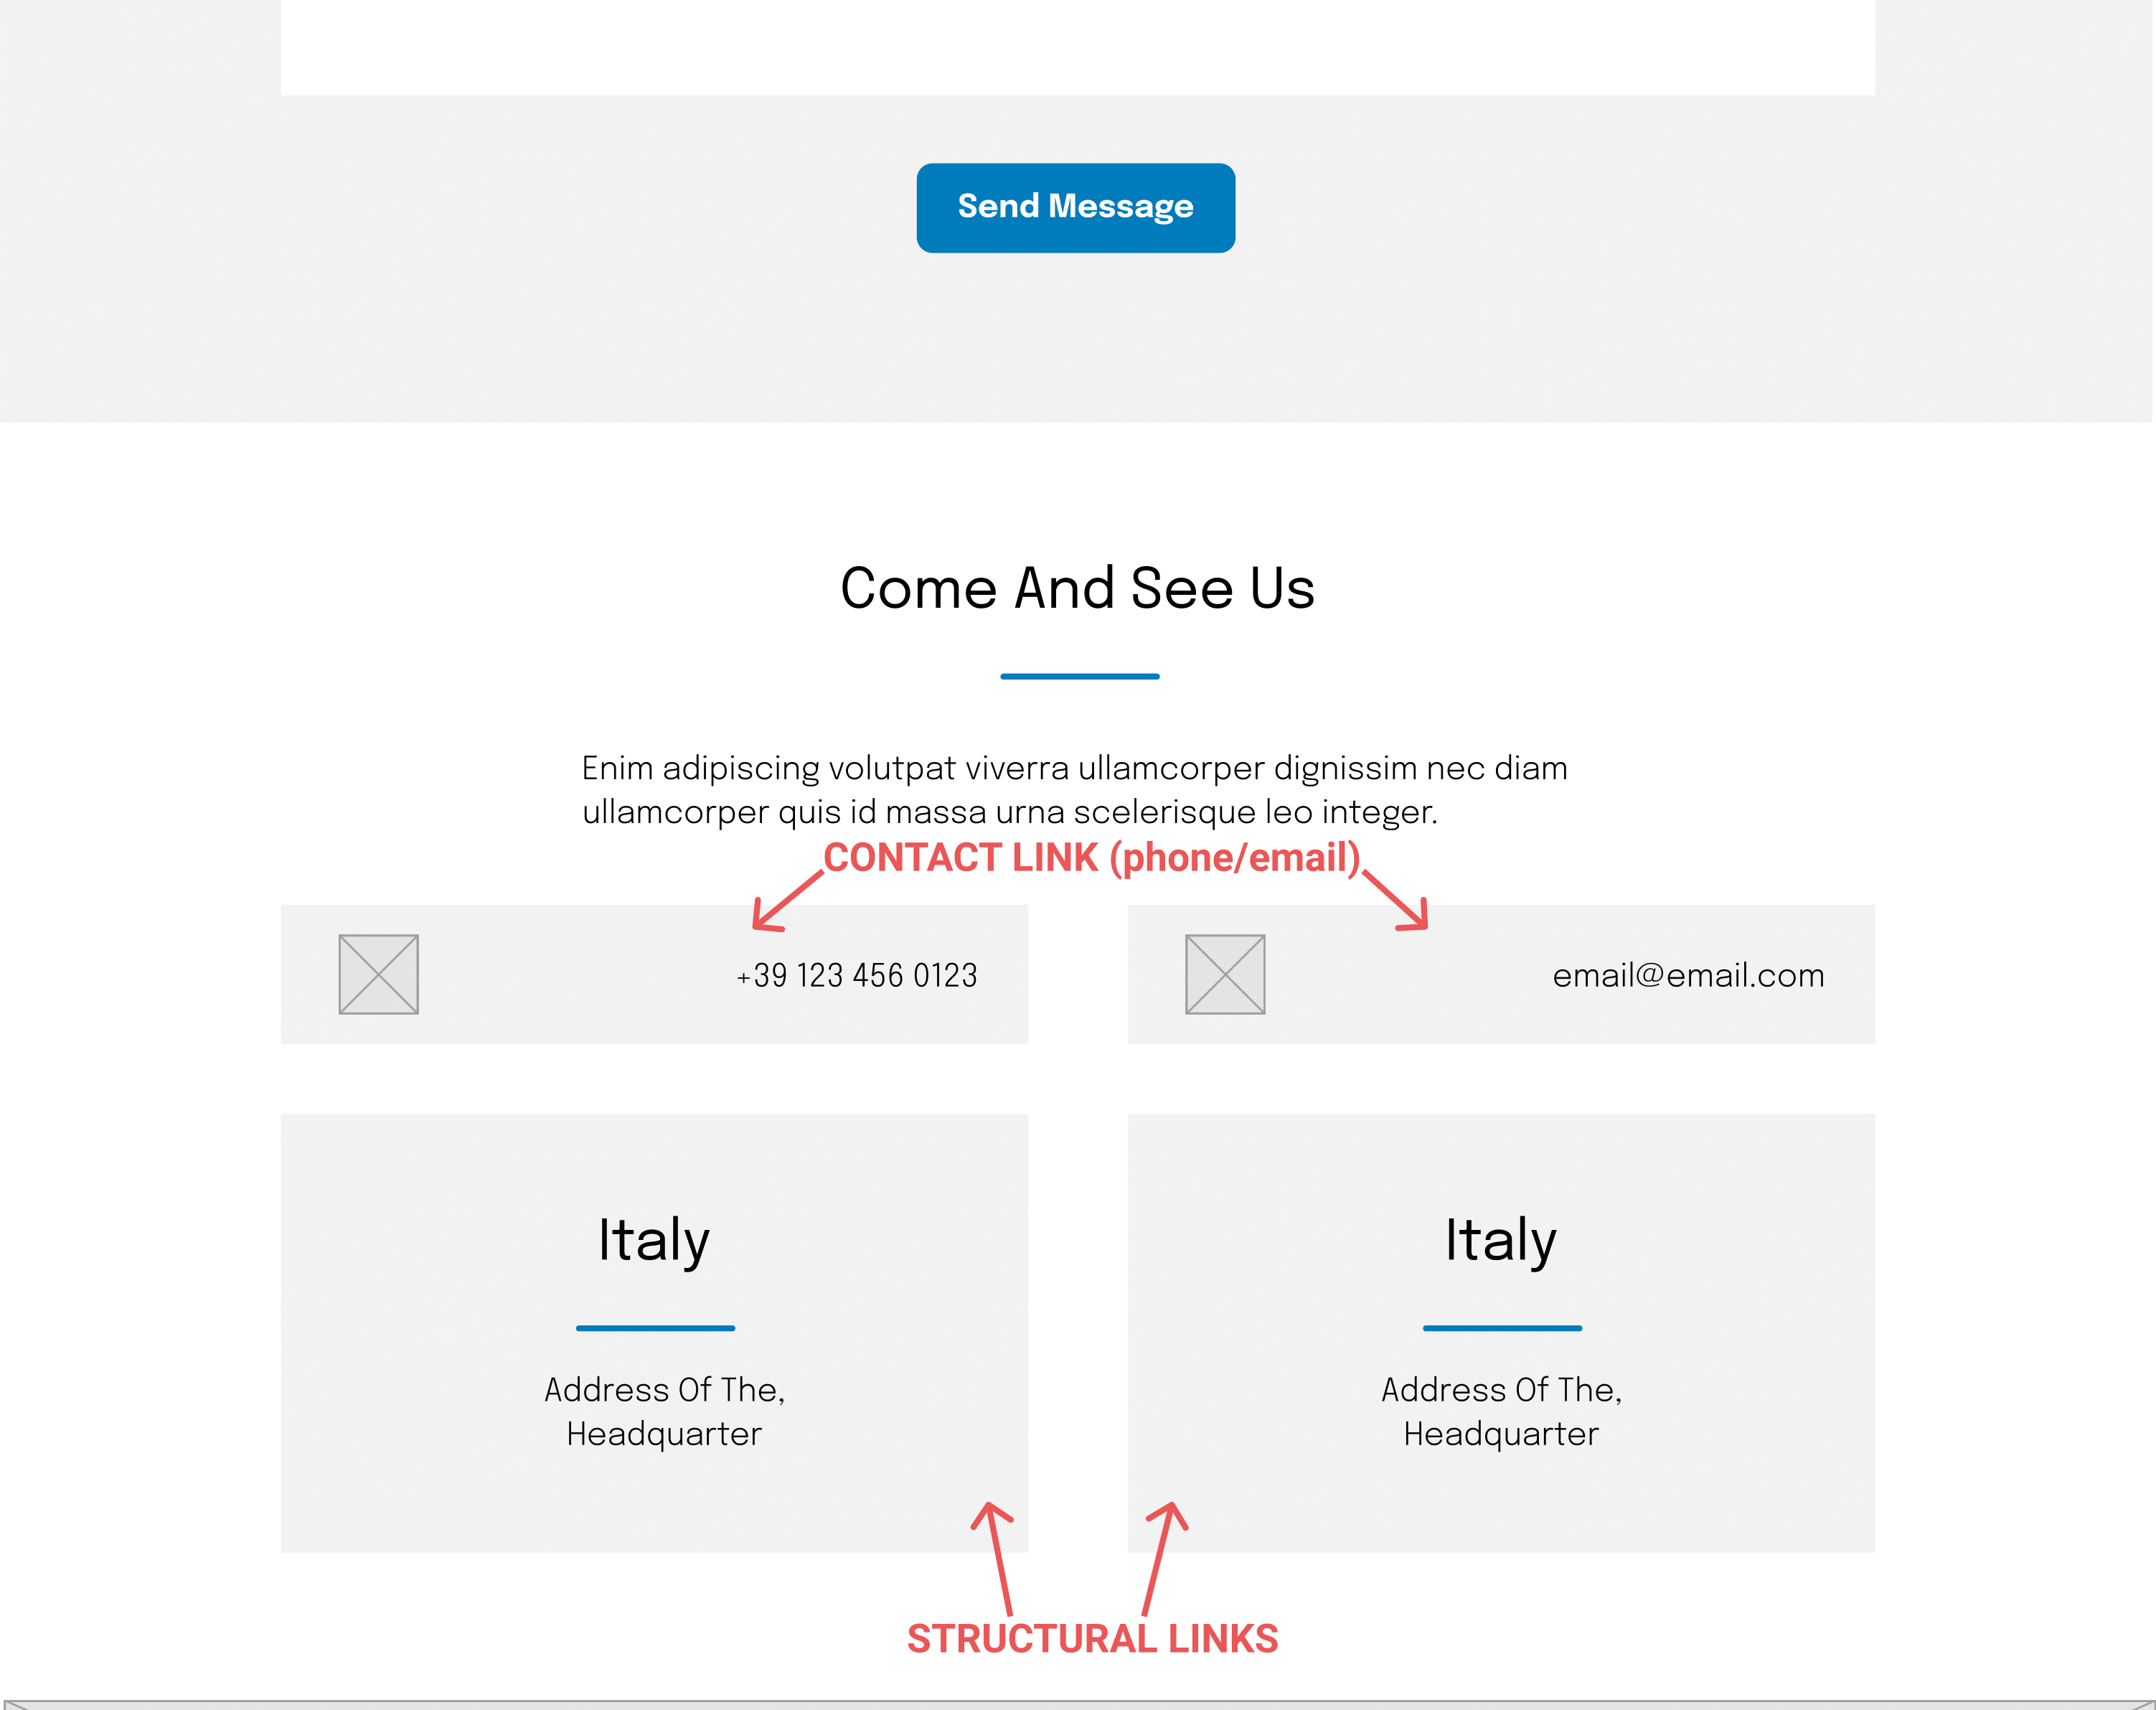
\includegraphics[width=0.45\textwidth]{low_fid_wireframes/contacts/2.png}
	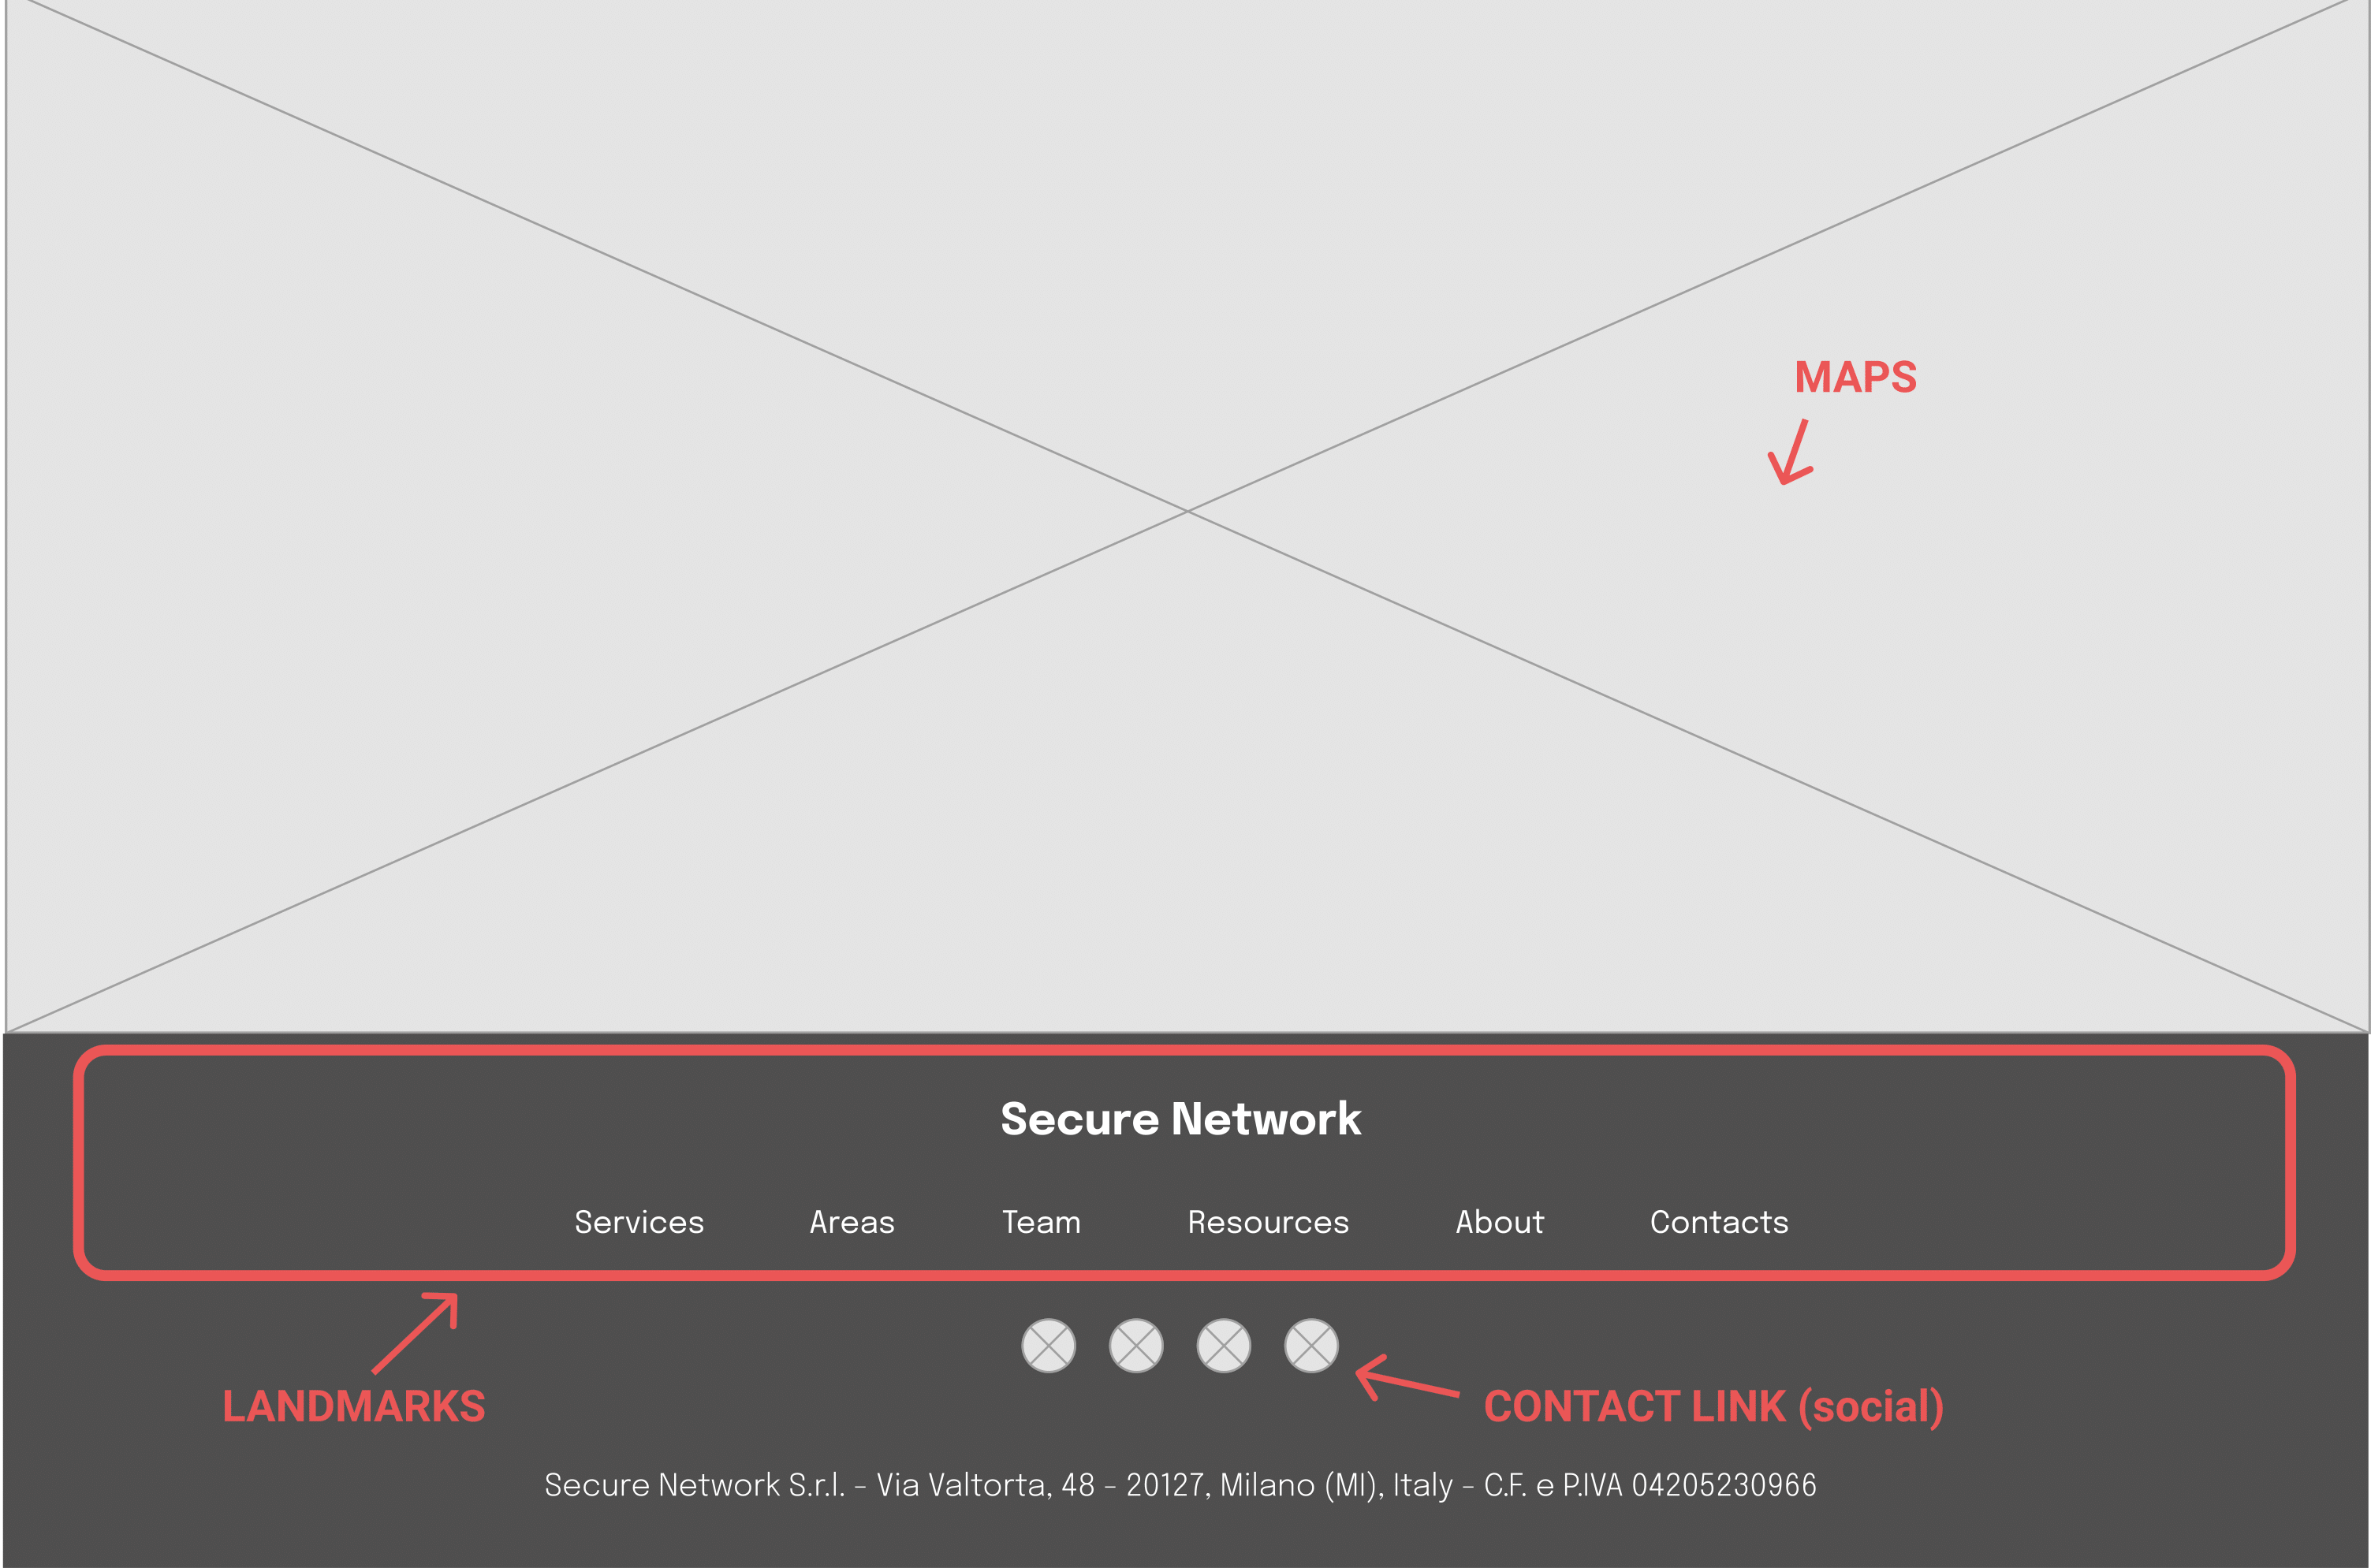
\includegraphics[width=0.45\textwidth]{low_fid_wireframes/contacts/3.png}
	\caption{Commented wireframes for the Contacts page.}
\end{figure}

\subsection{Kind of Topic: Area}

\begin{figure}[H]
	\centering
	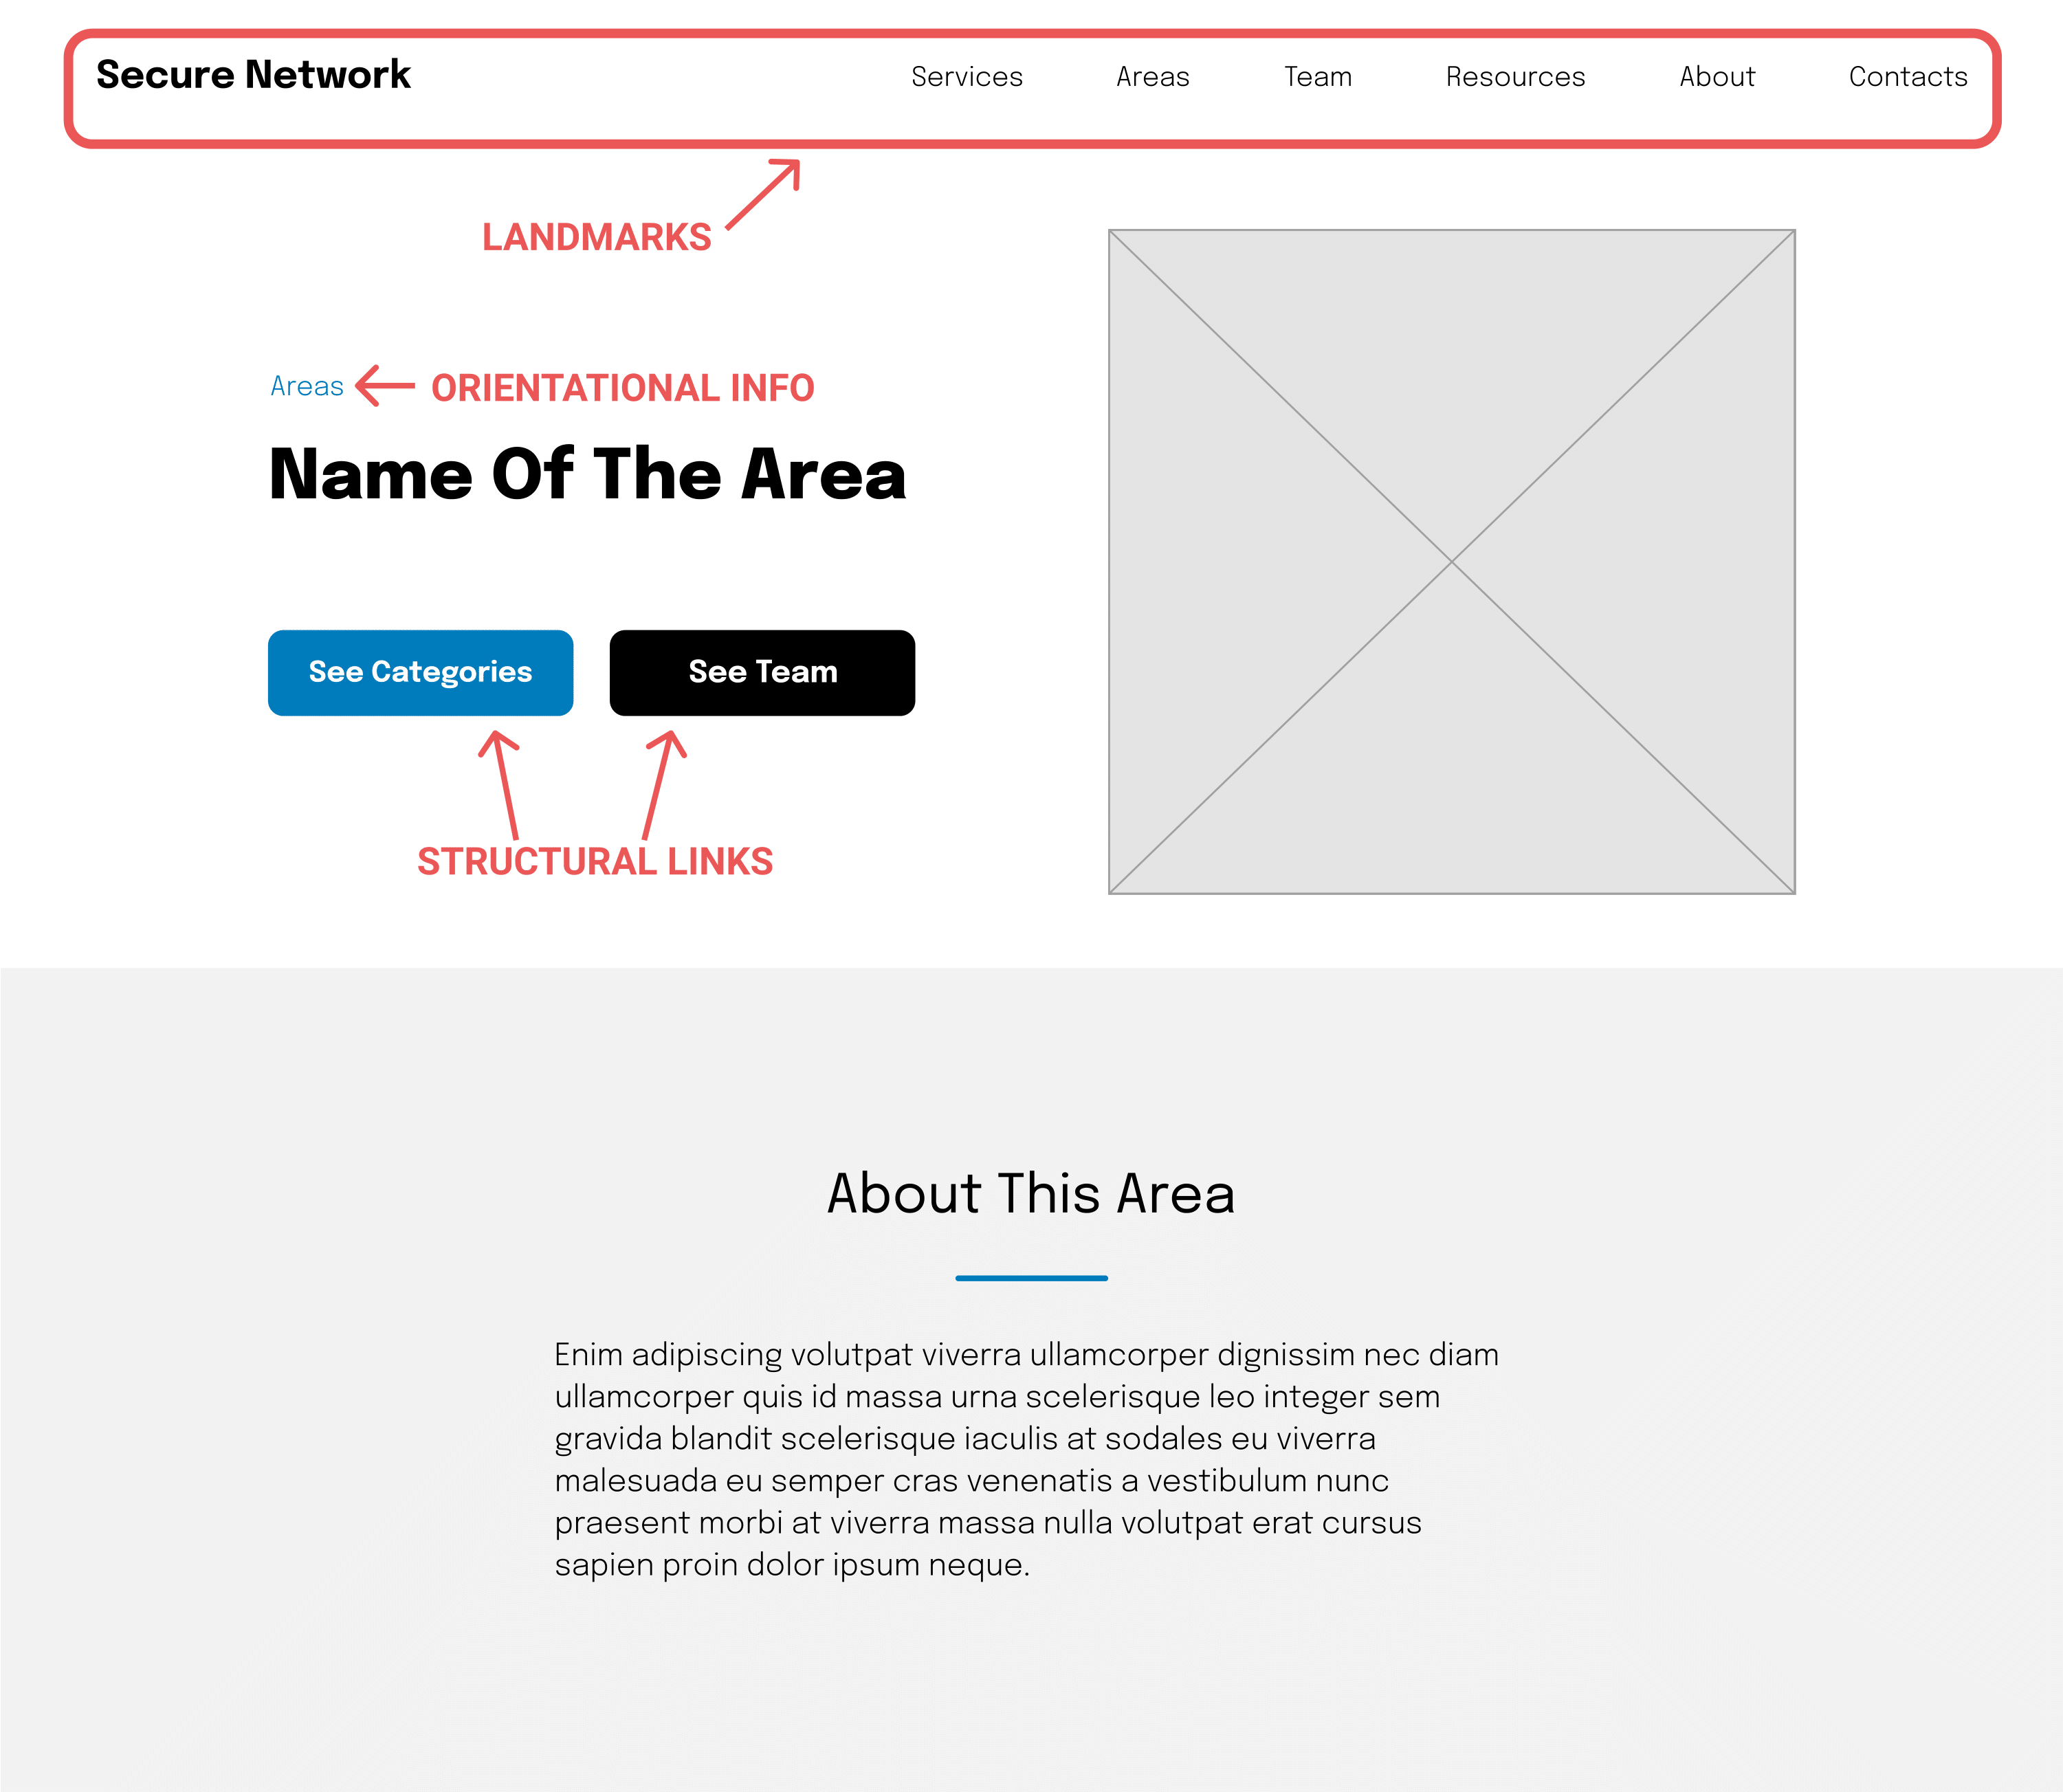
\includegraphics[width=0.45\textwidth]{low_fid_wireframes/area/1.png}
	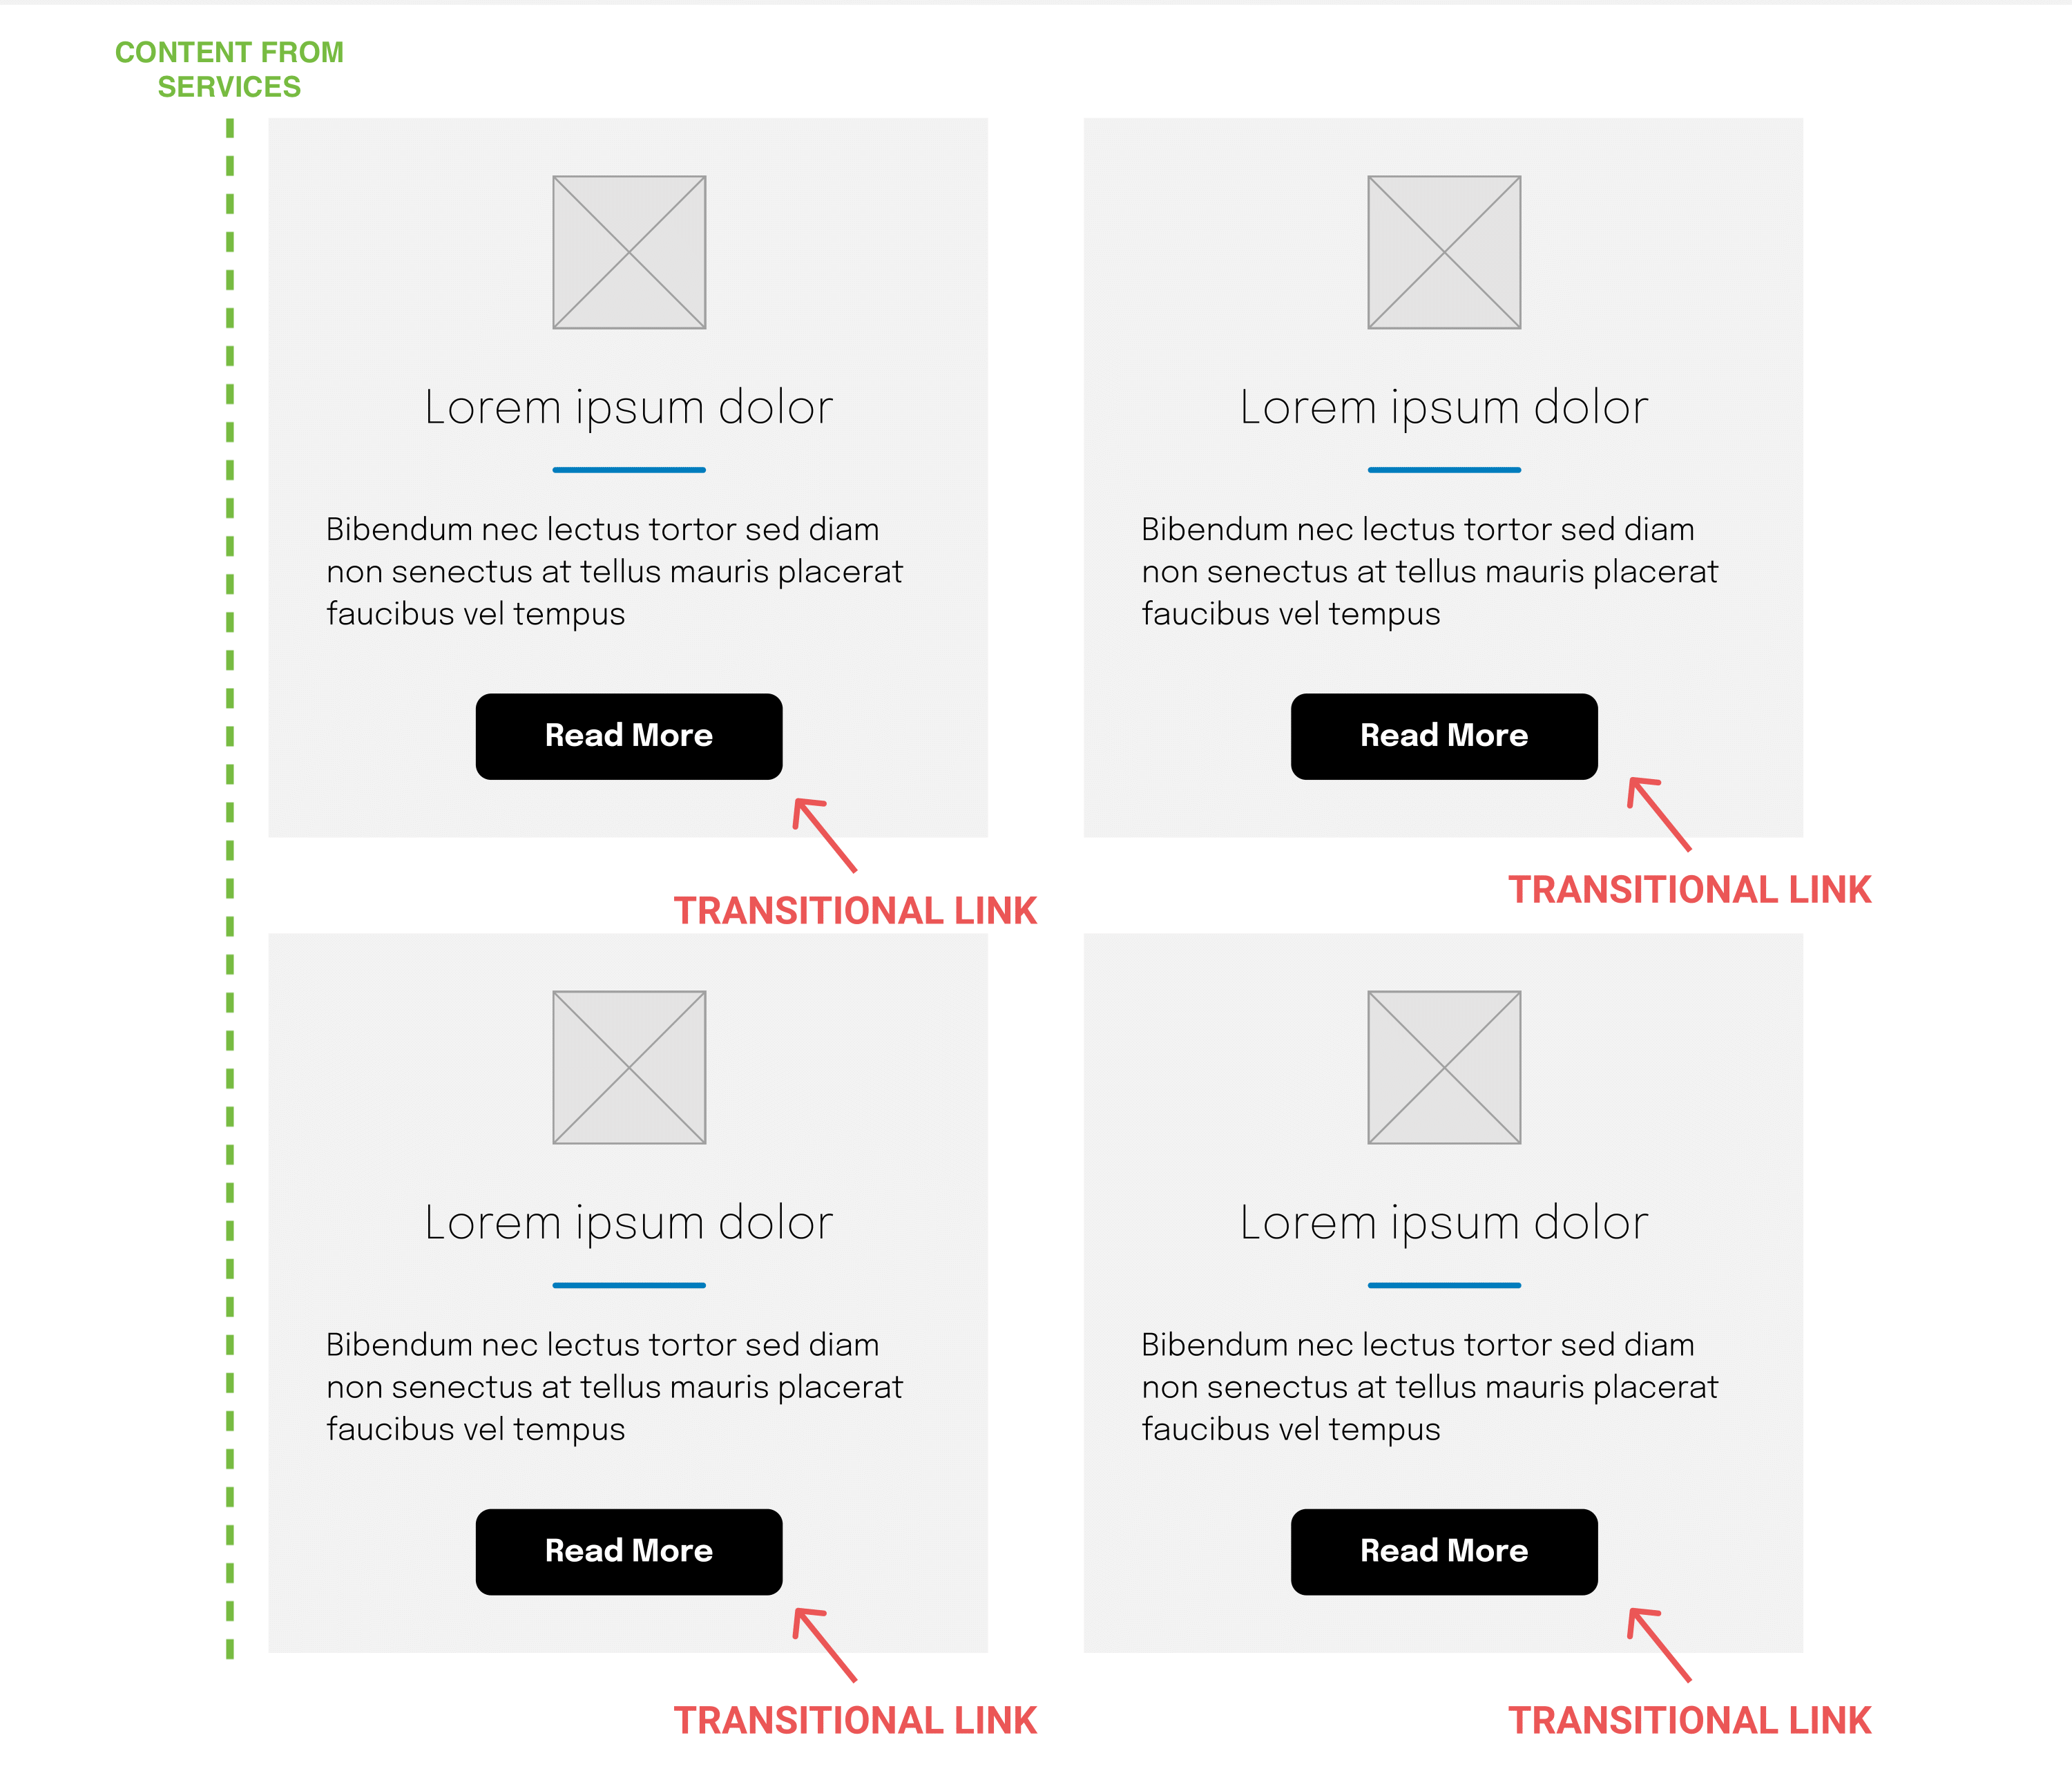
\includegraphics[width=0.45\textwidth]{low_fid_wireframes/area/2.png}
	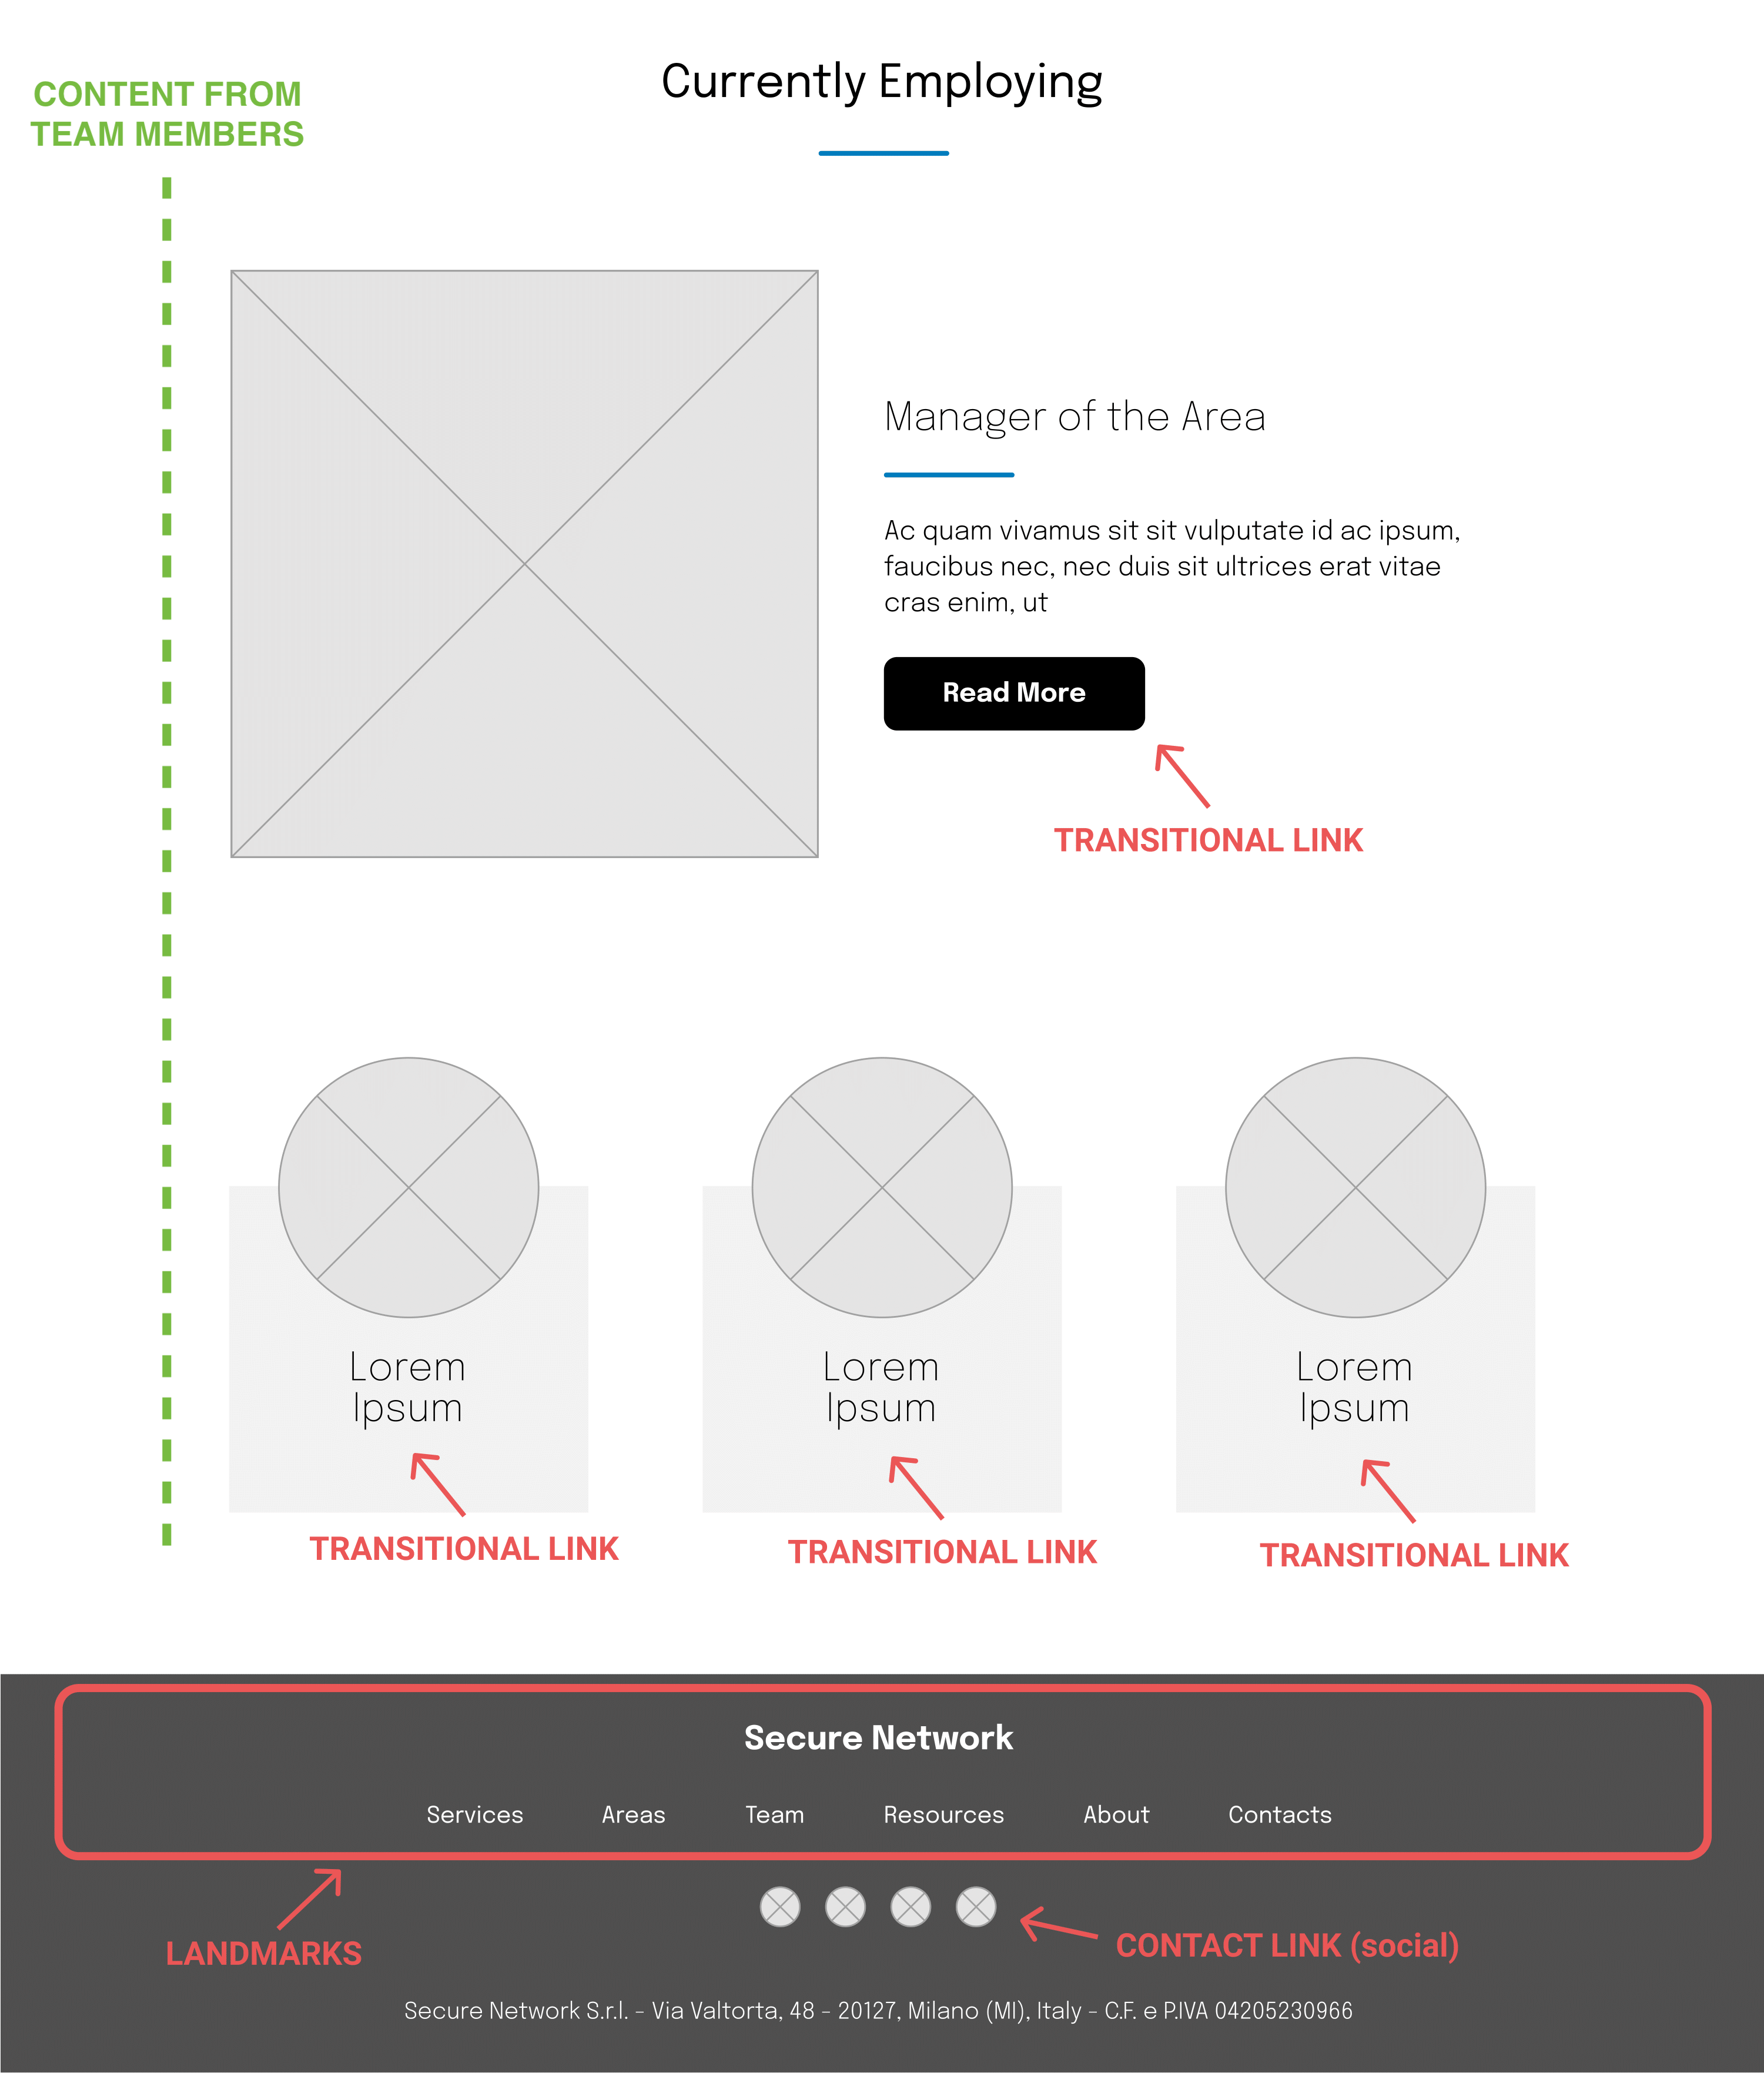
\includegraphics[width=0.45\textwidth]{low_fid_wireframes/area/3.png}
	\caption{Commented wireframes for the Area page.}
\end{figure}

\subsection{Kind of Topic: Person}

\begin{figure}[H]
	\centering
	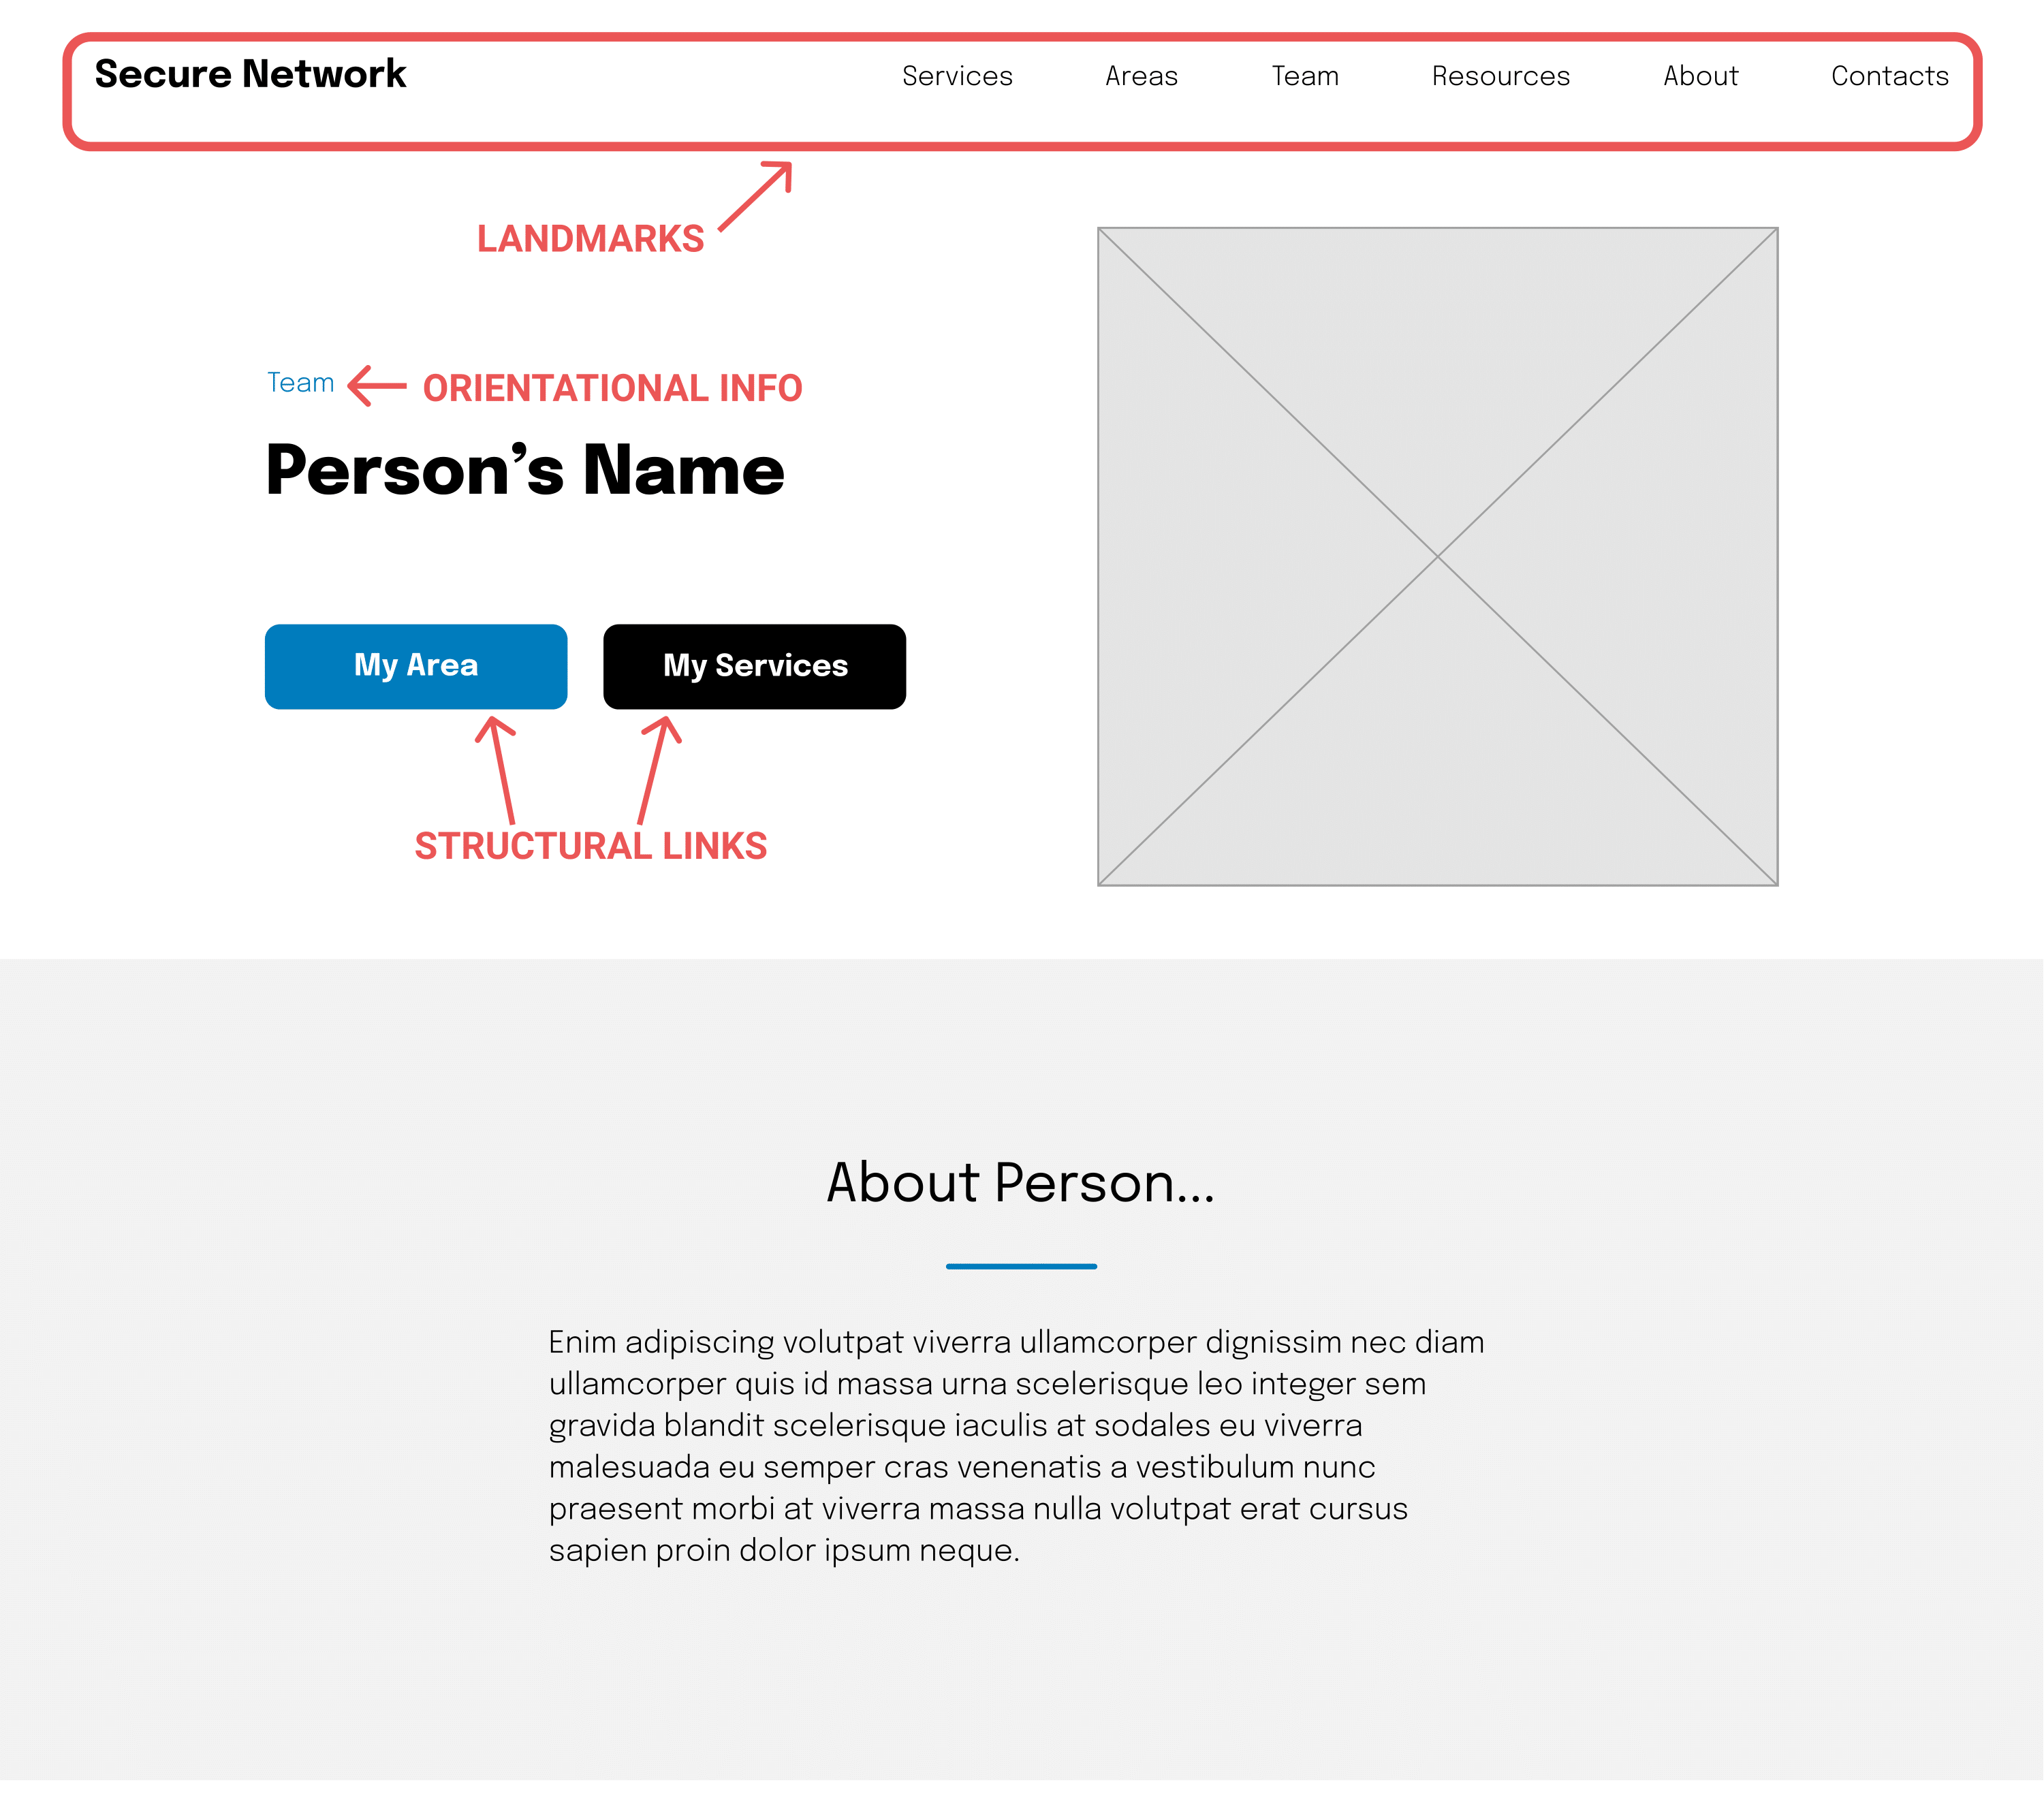
\includegraphics[width=0.45\textwidth]{low_fid_wireframes/person/1.png}
	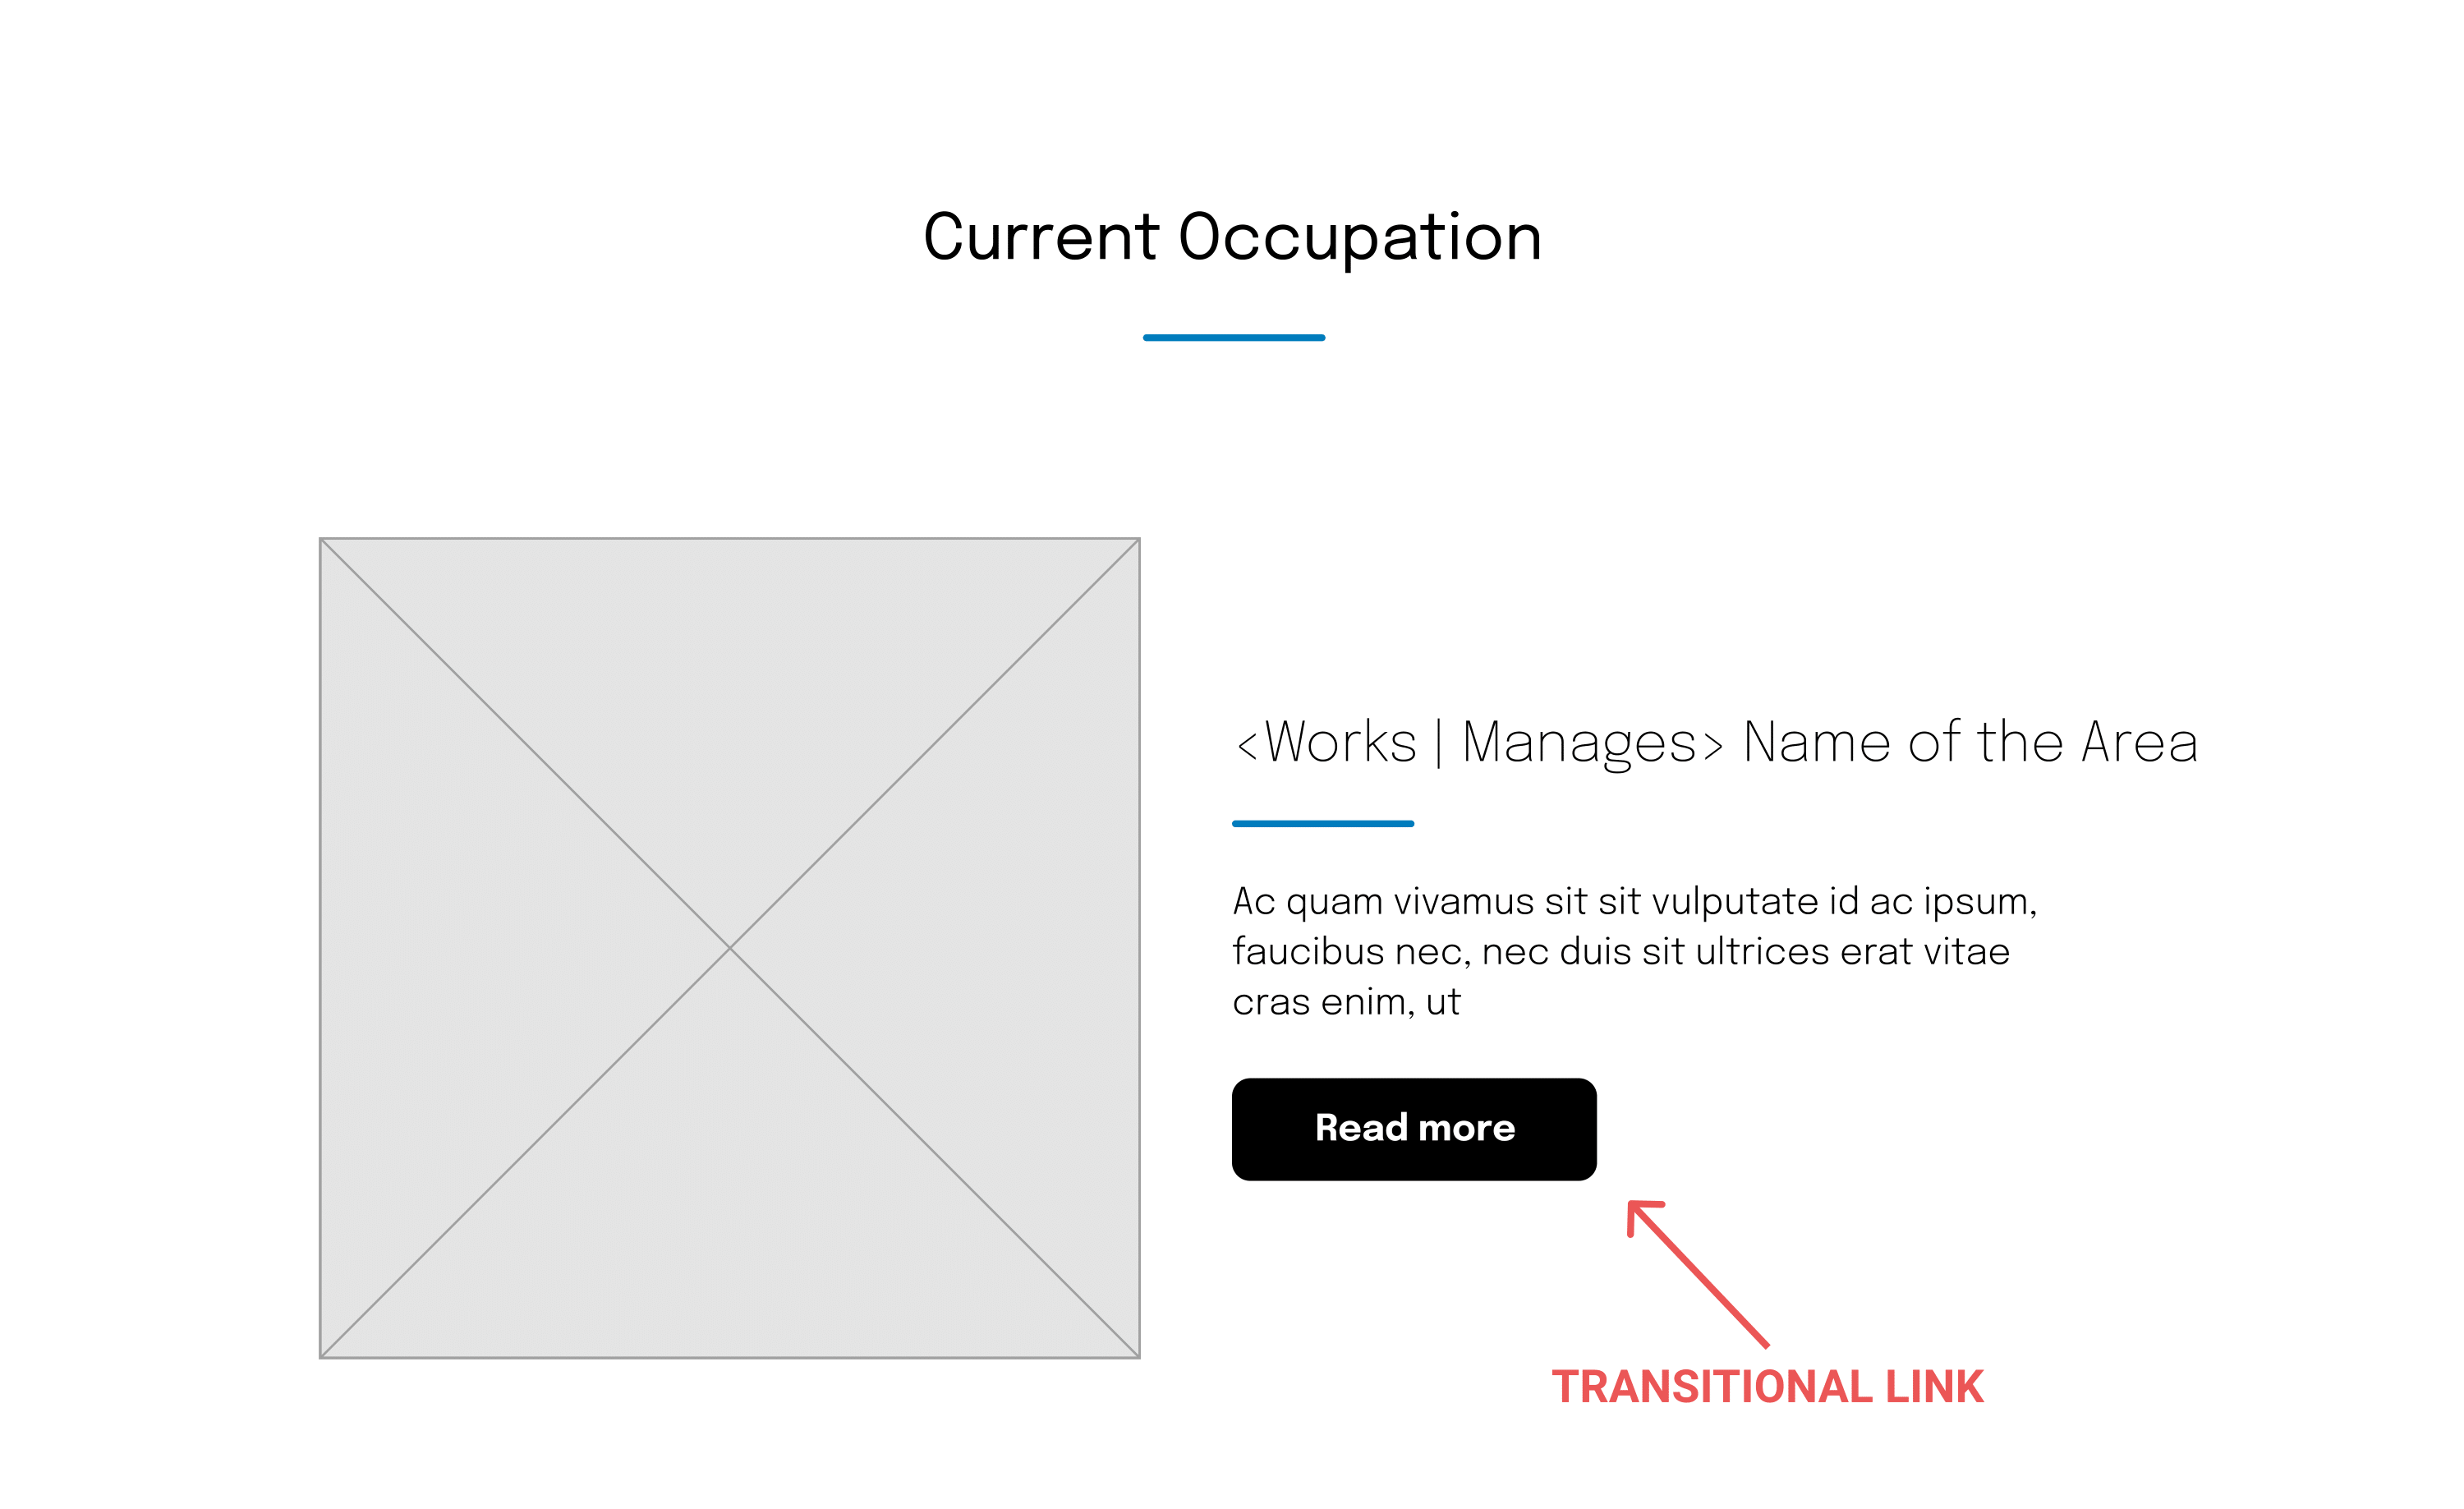
\includegraphics[width=0.45\textwidth]{low_fid_wireframes/person/2.png}
	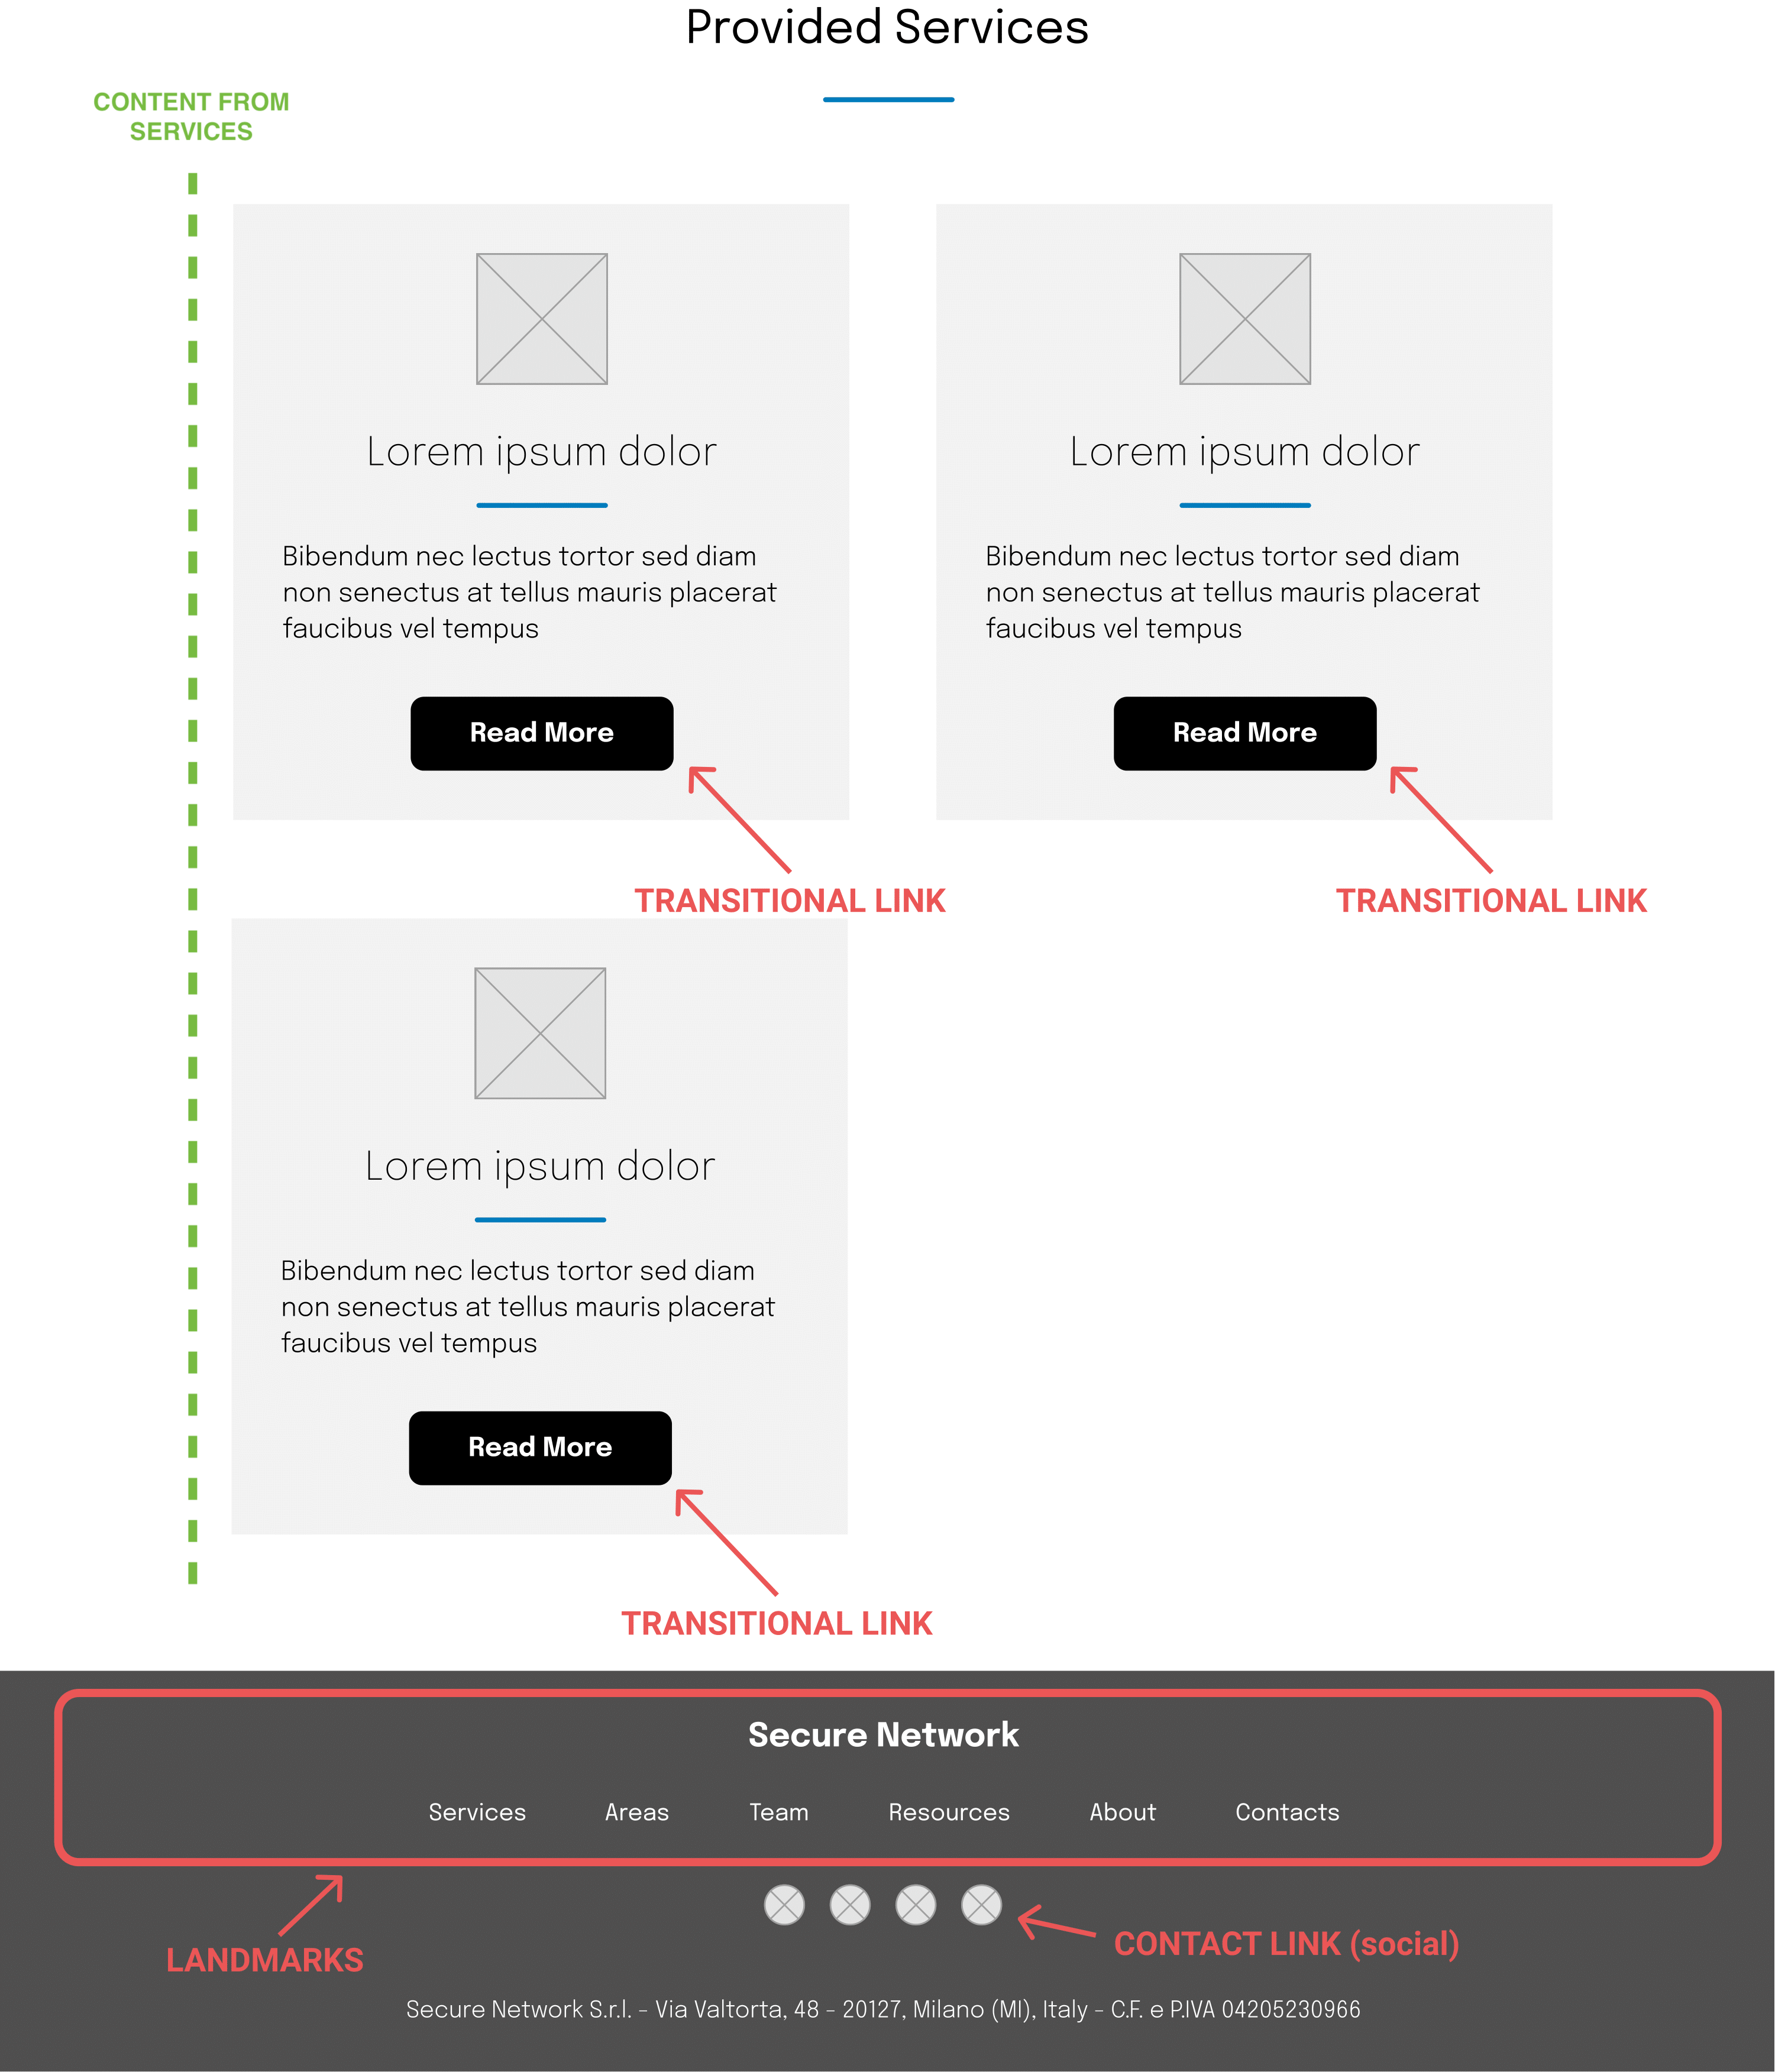
\includegraphics[width=0.45\textwidth]{low_fid_wireframes/person/3.png}
	\caption{Commented wireframes for the Person page.}
\end{figure}

\subsection{Kind of Topic: Service}

\begin{figure}[H]
	\centering
	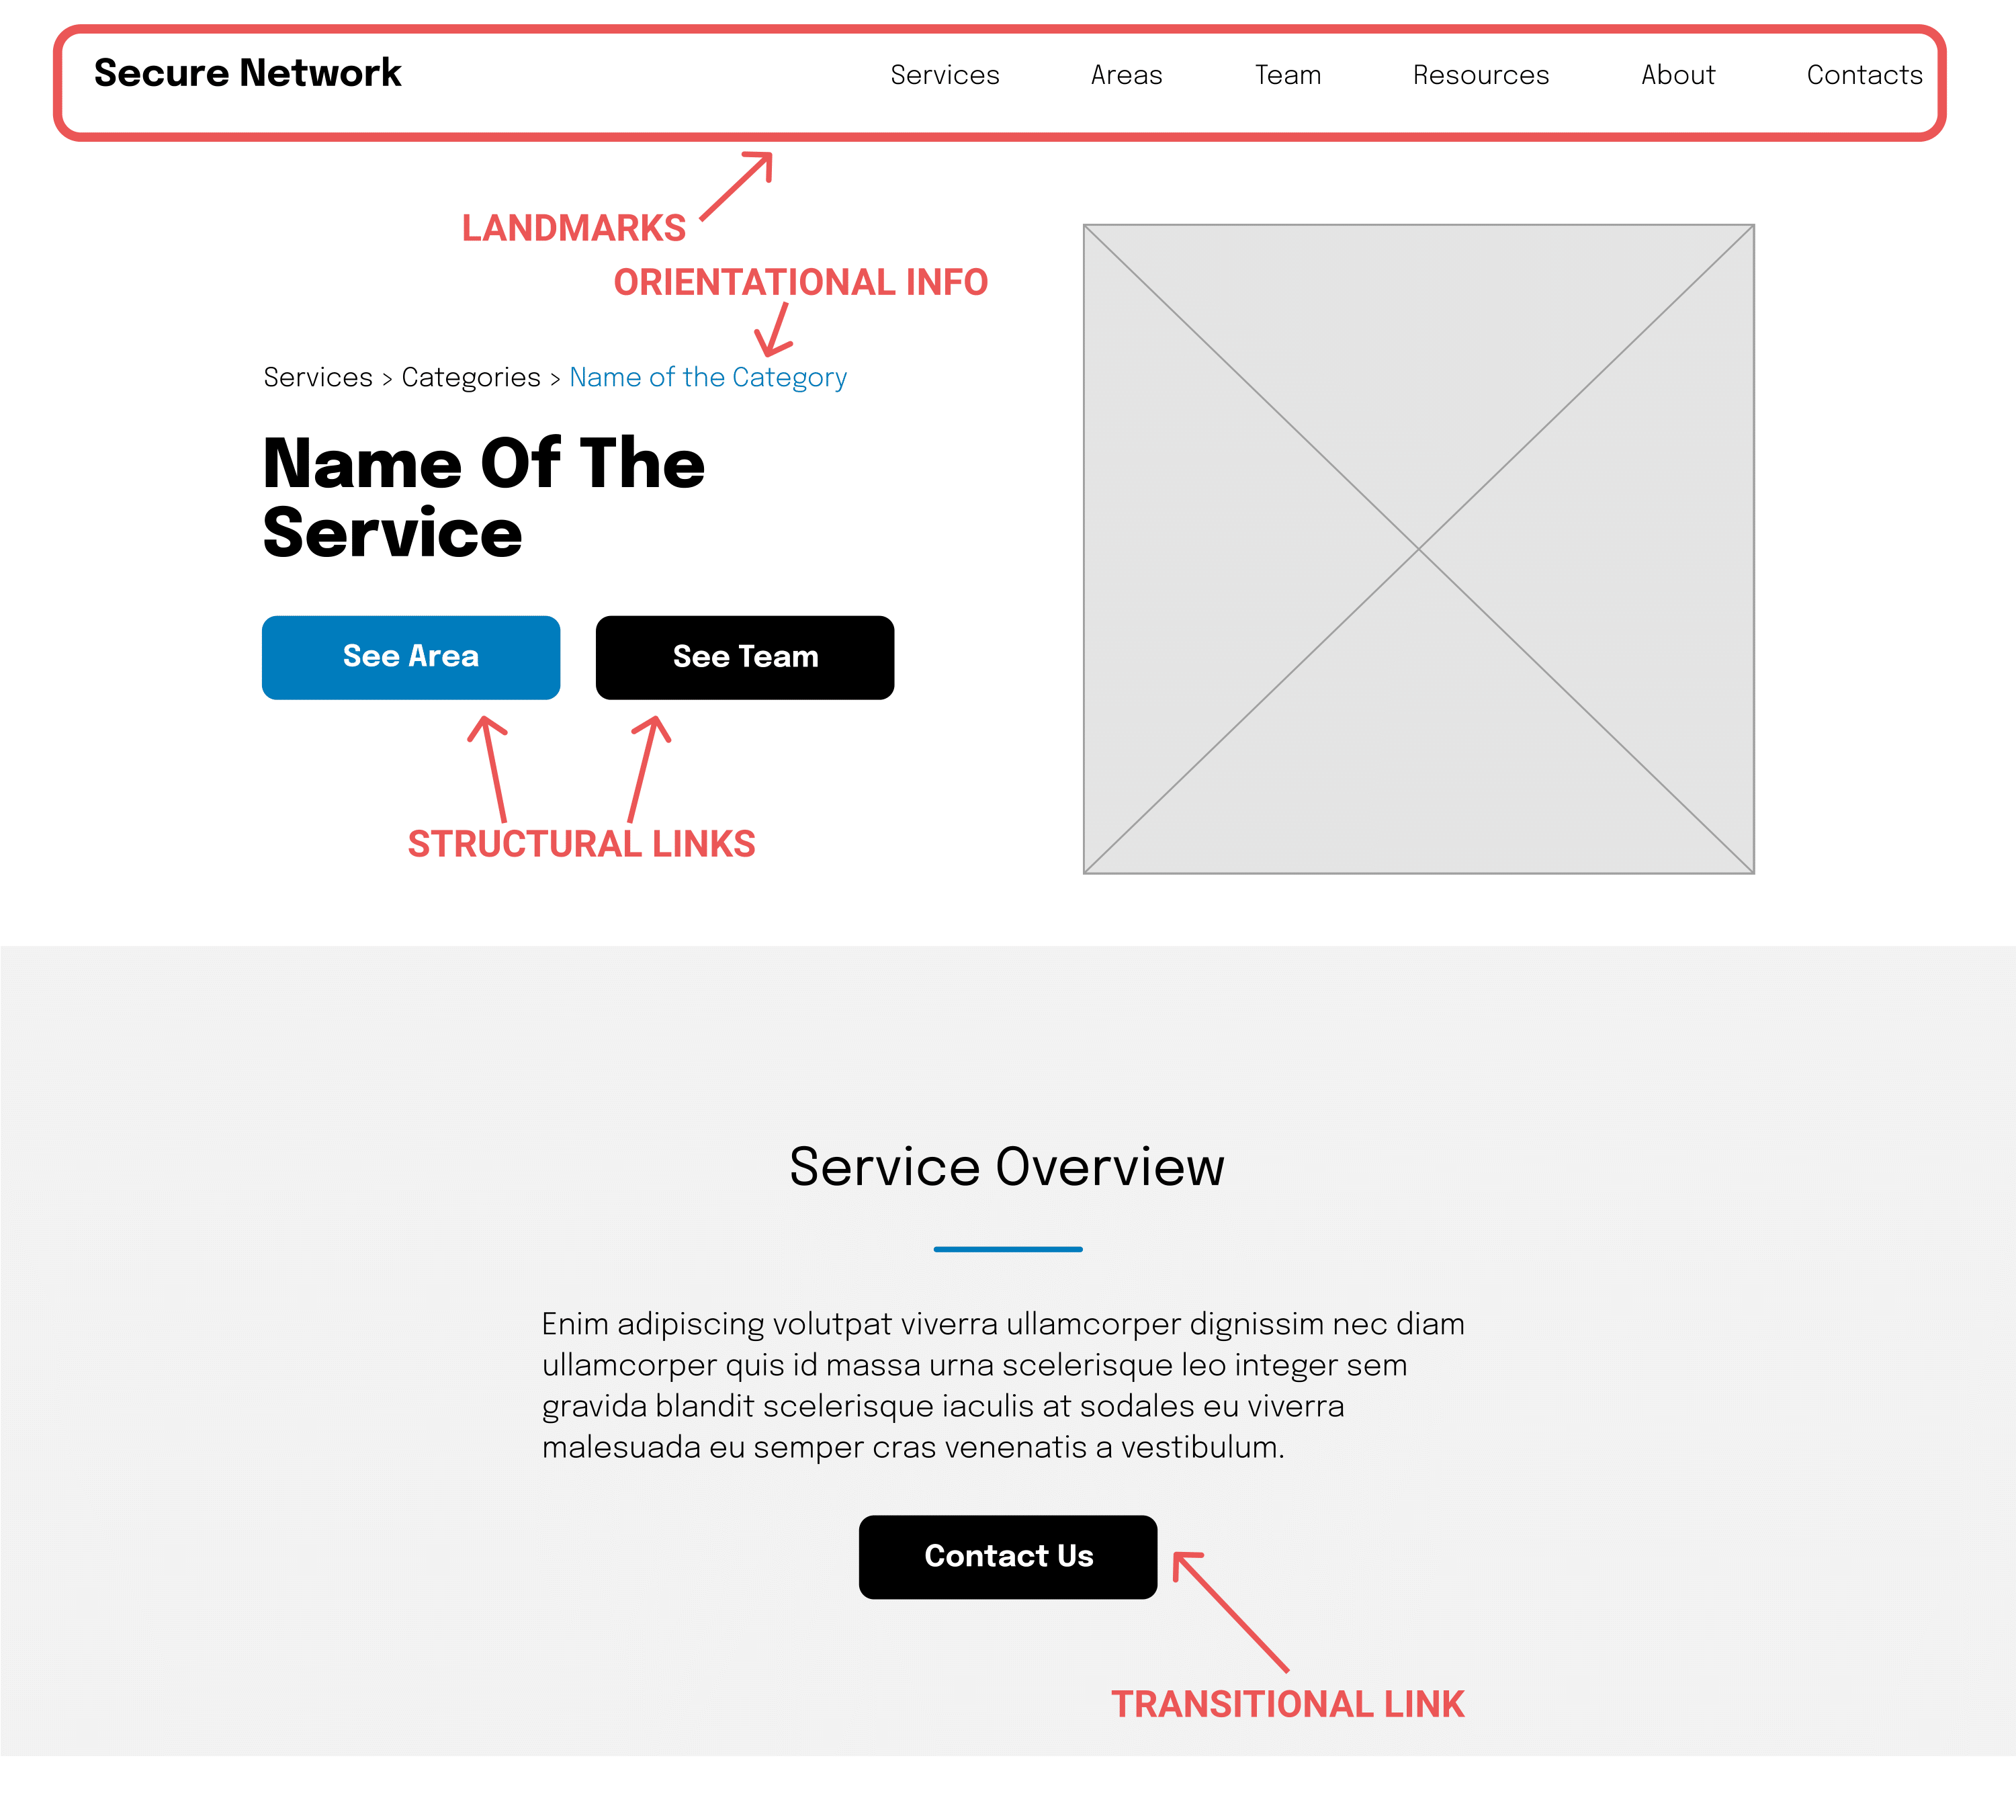
\includegraphics[width=0.45\textwidth]{low_fid_wireframes/service/1.png}
	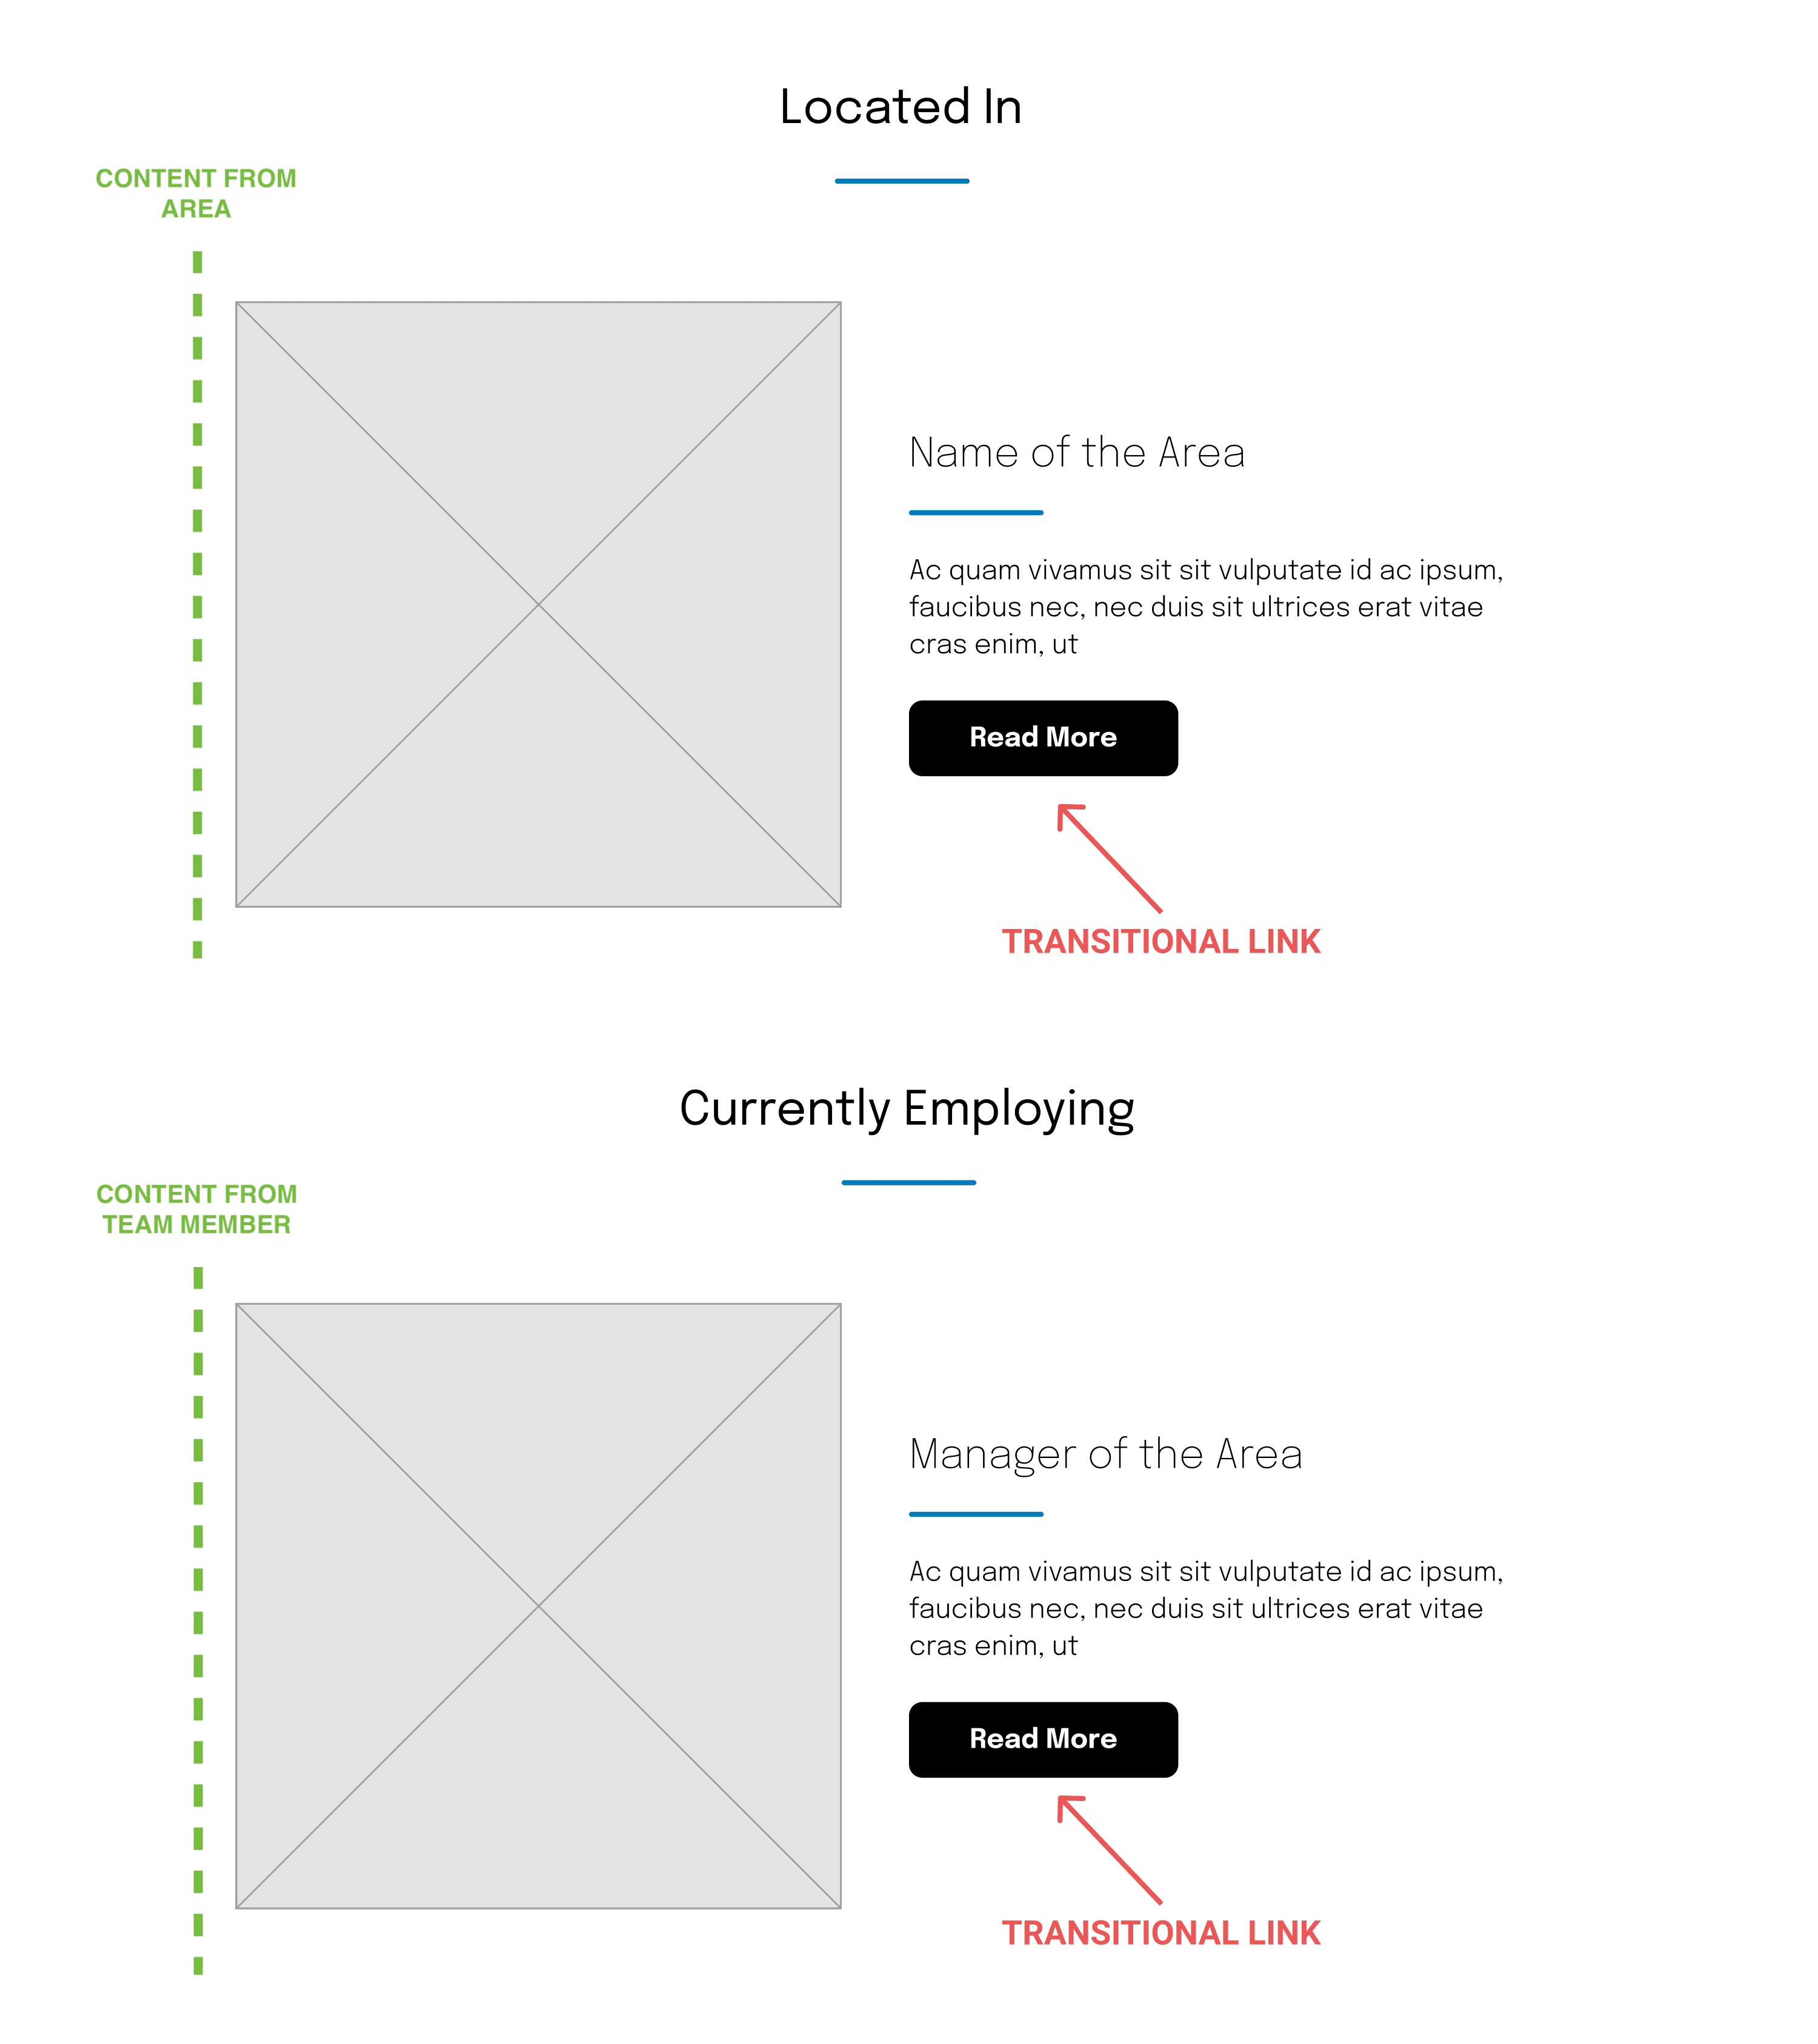
\includegraphics[width=0.45\textwidth]{low_fid_wireframes/service/2.png}
	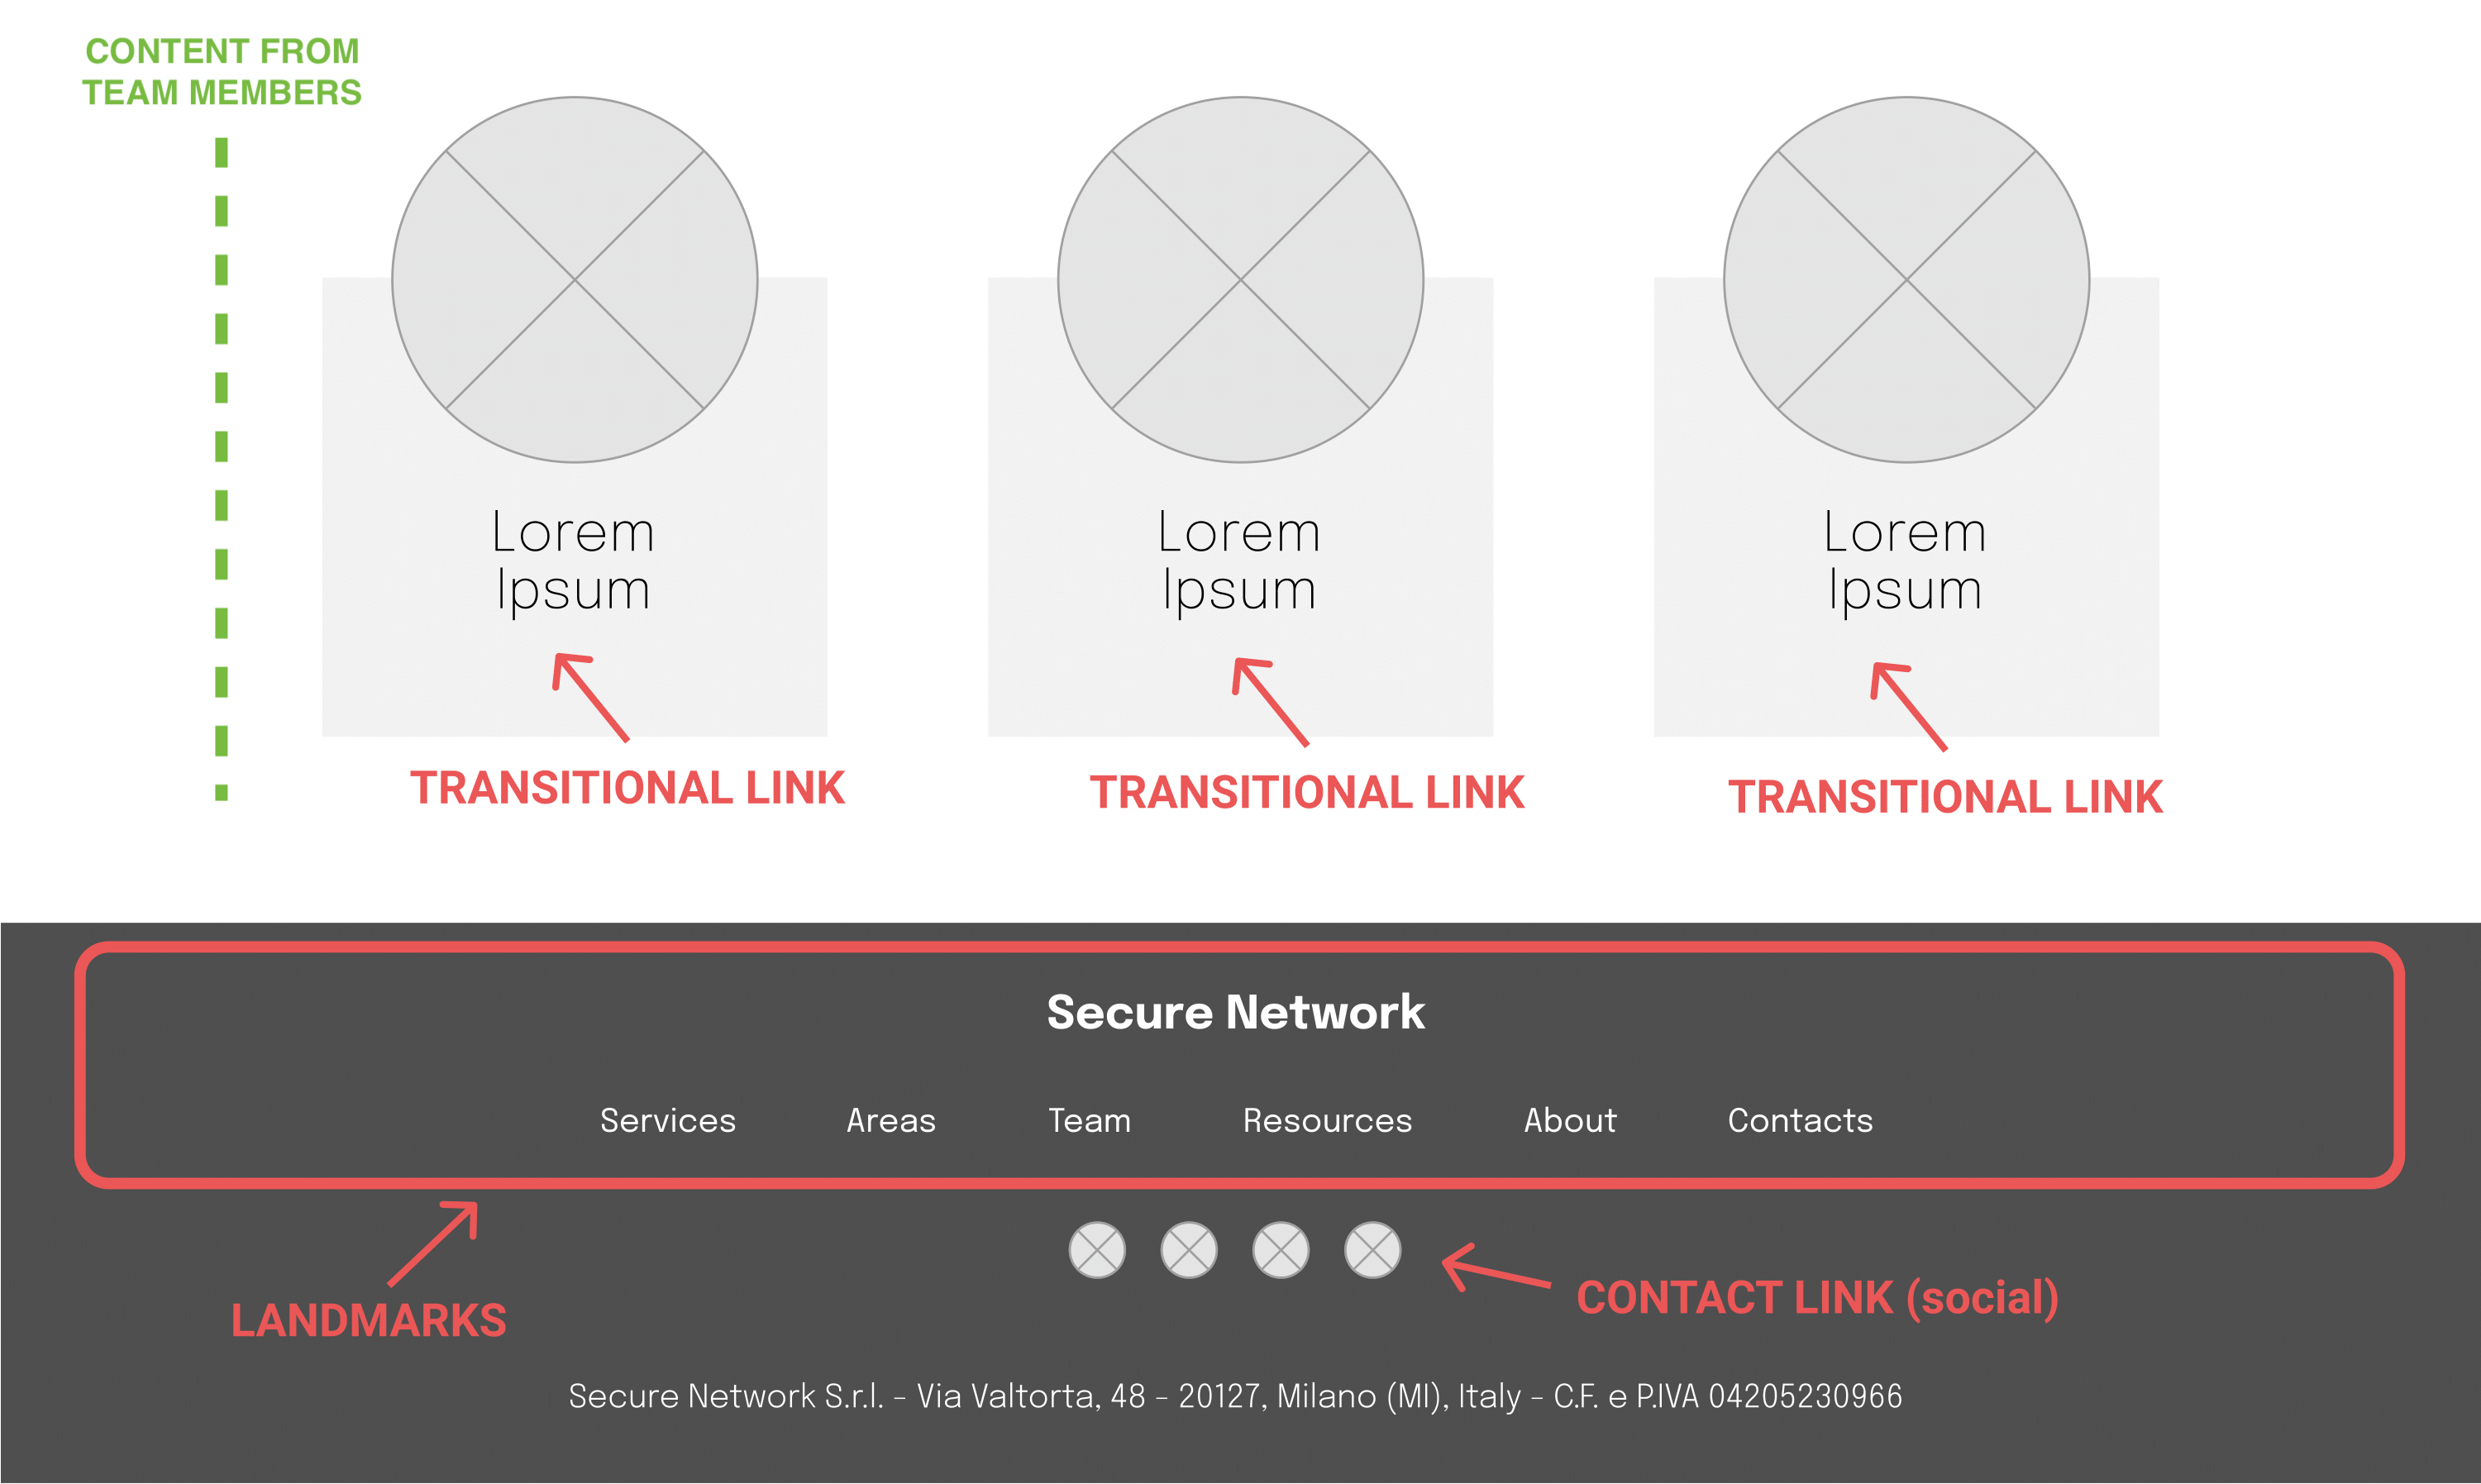
\includegraphics[width=0.45\textwidth]{low_fid_wireframes/service/3.png}
	\caption{Commented wireframes for the Service page.}
\end{figure}

\subsection{Kind of Topic: Resource}

\begin{figure}[H]
	\centering
	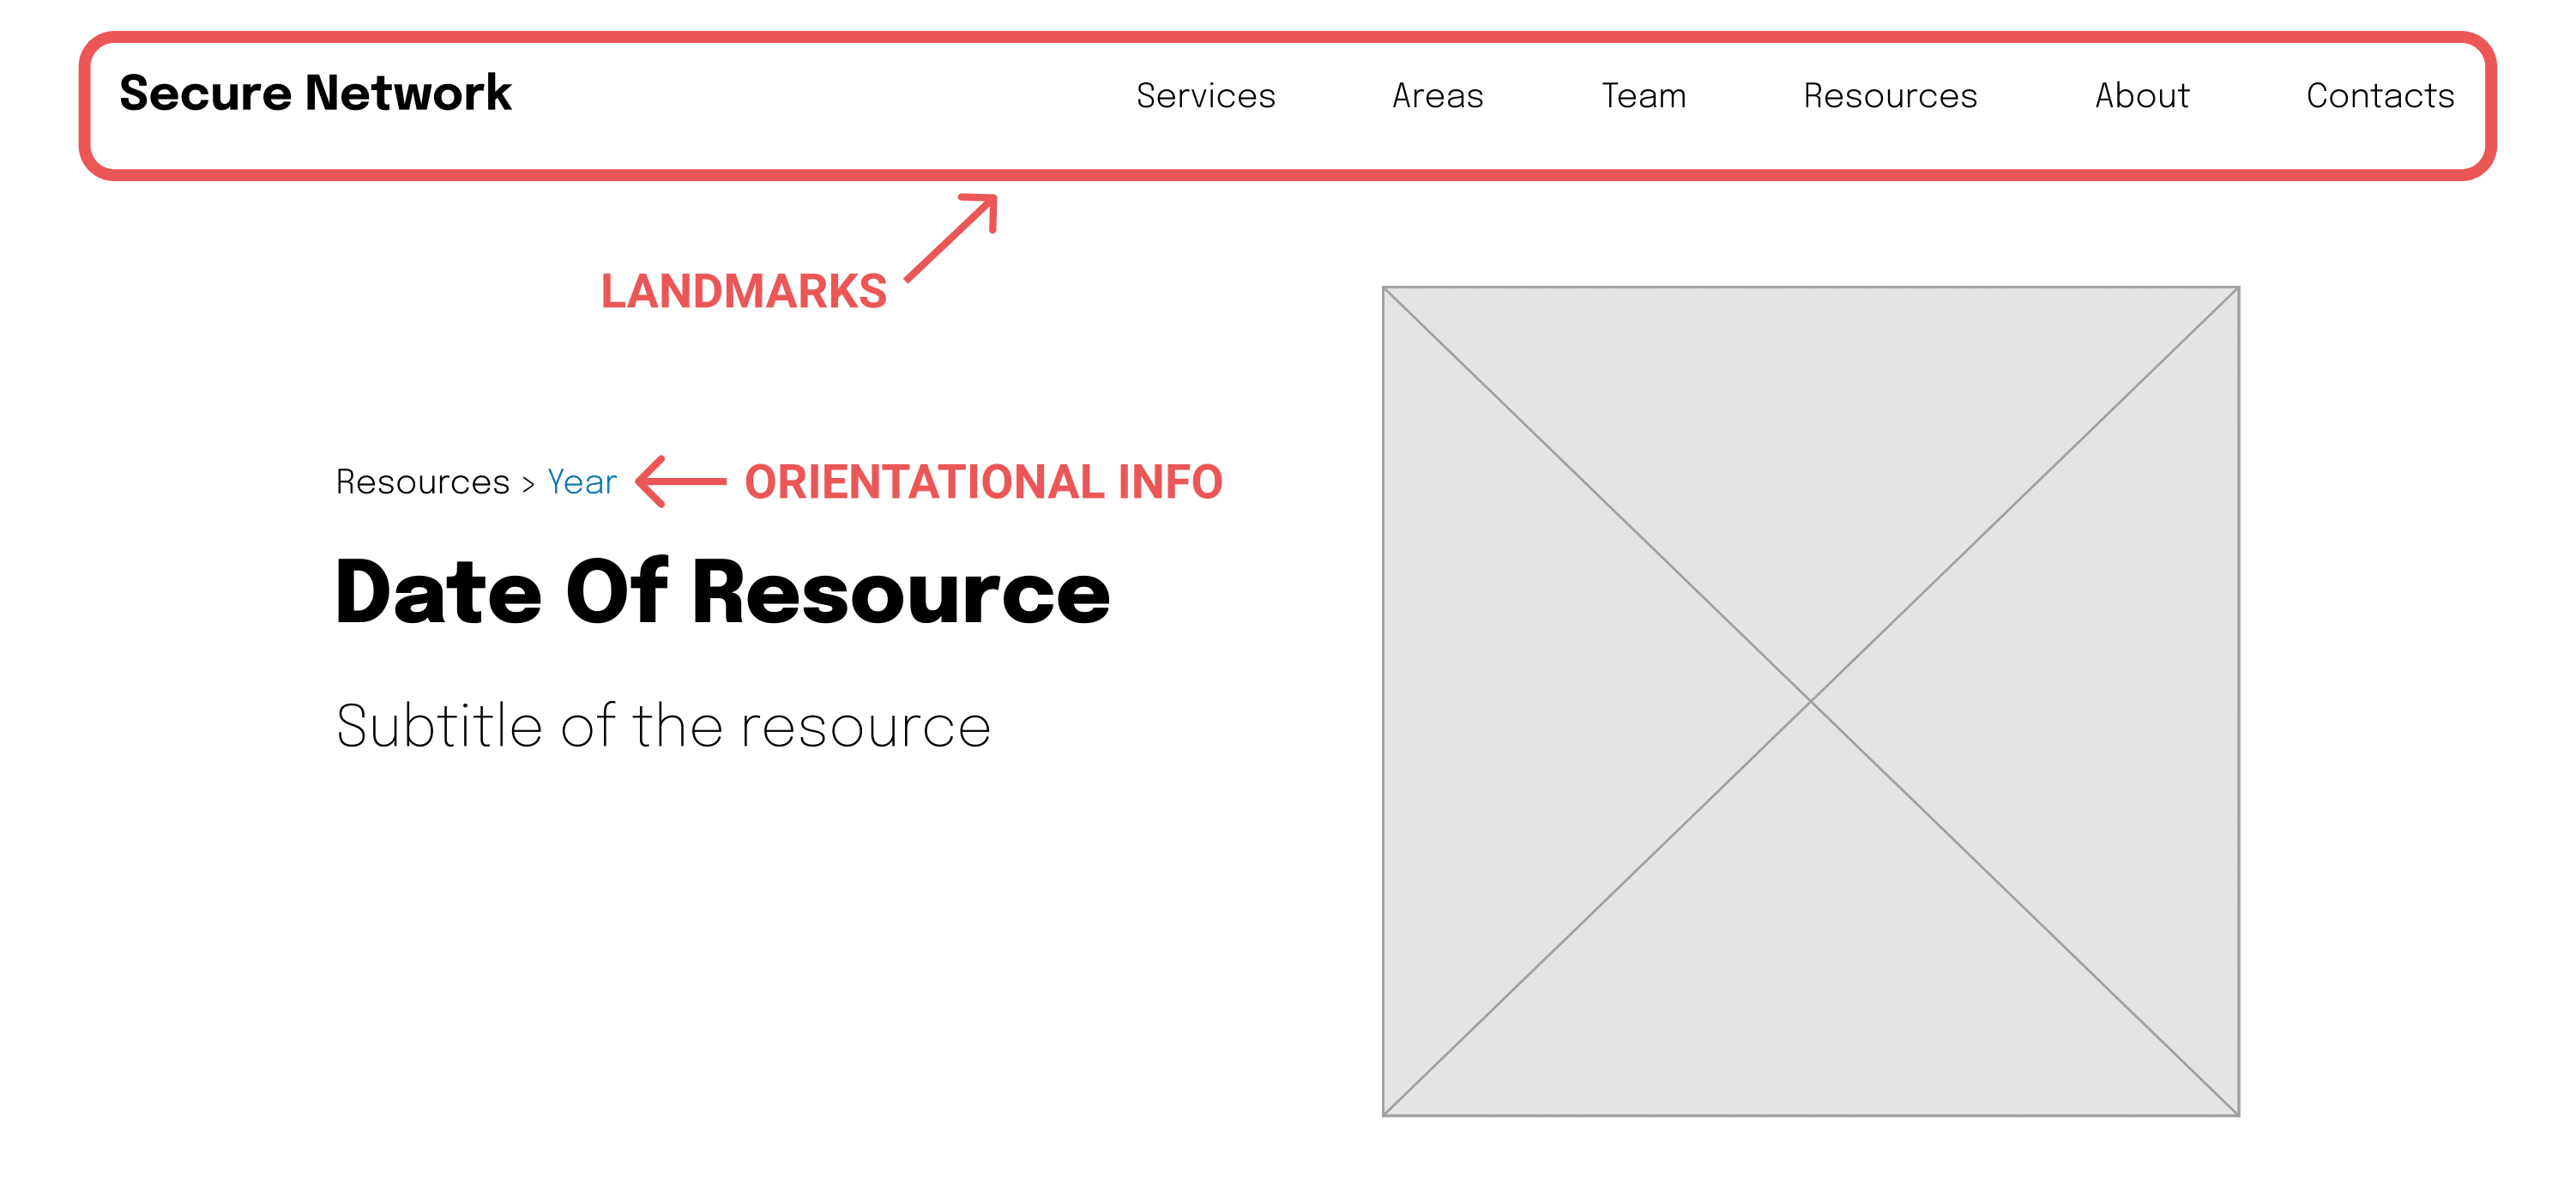
\includegraphics[width=0.45\textwidth]{low_fid_wireframes/resource/1.png}
	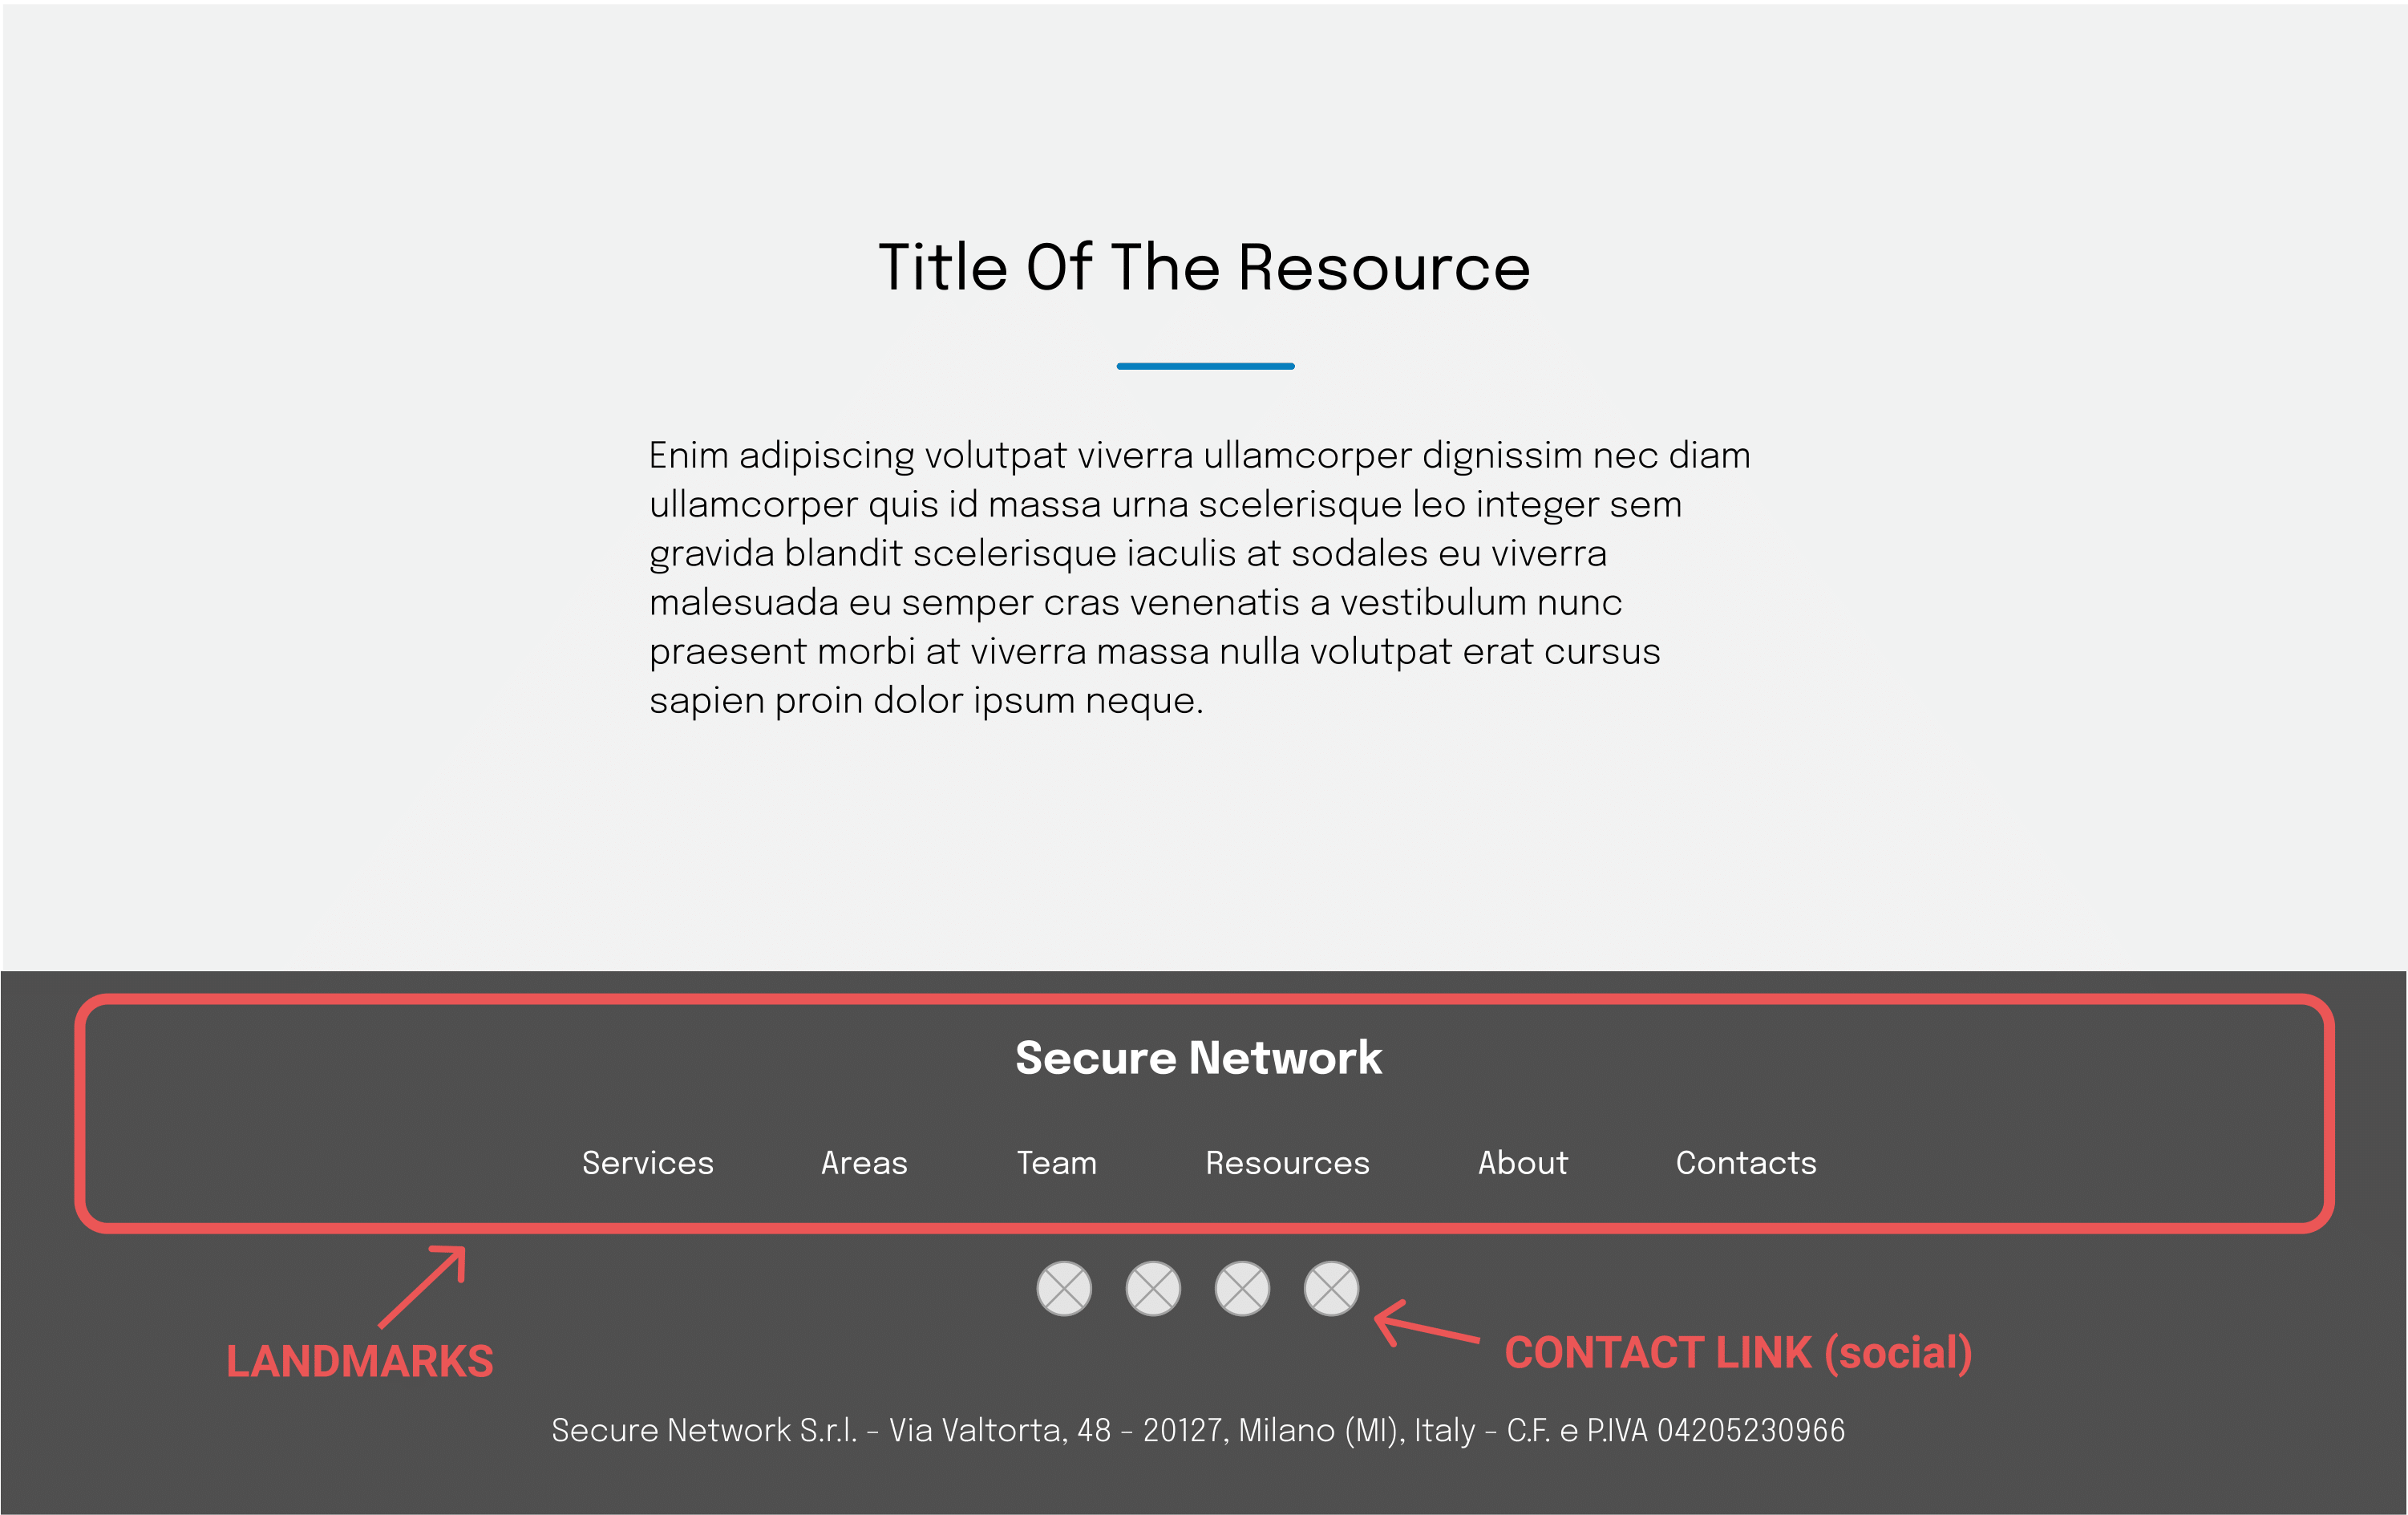
\includegraphics[width=0.45\textwidth]{low_fid_wireframes/resource/2.png}
	\caption{Commented wireframes for the Resources page.}
\end{figure}

\subsection{Group: Areas}

\begin{figure}[H]
	\centering
	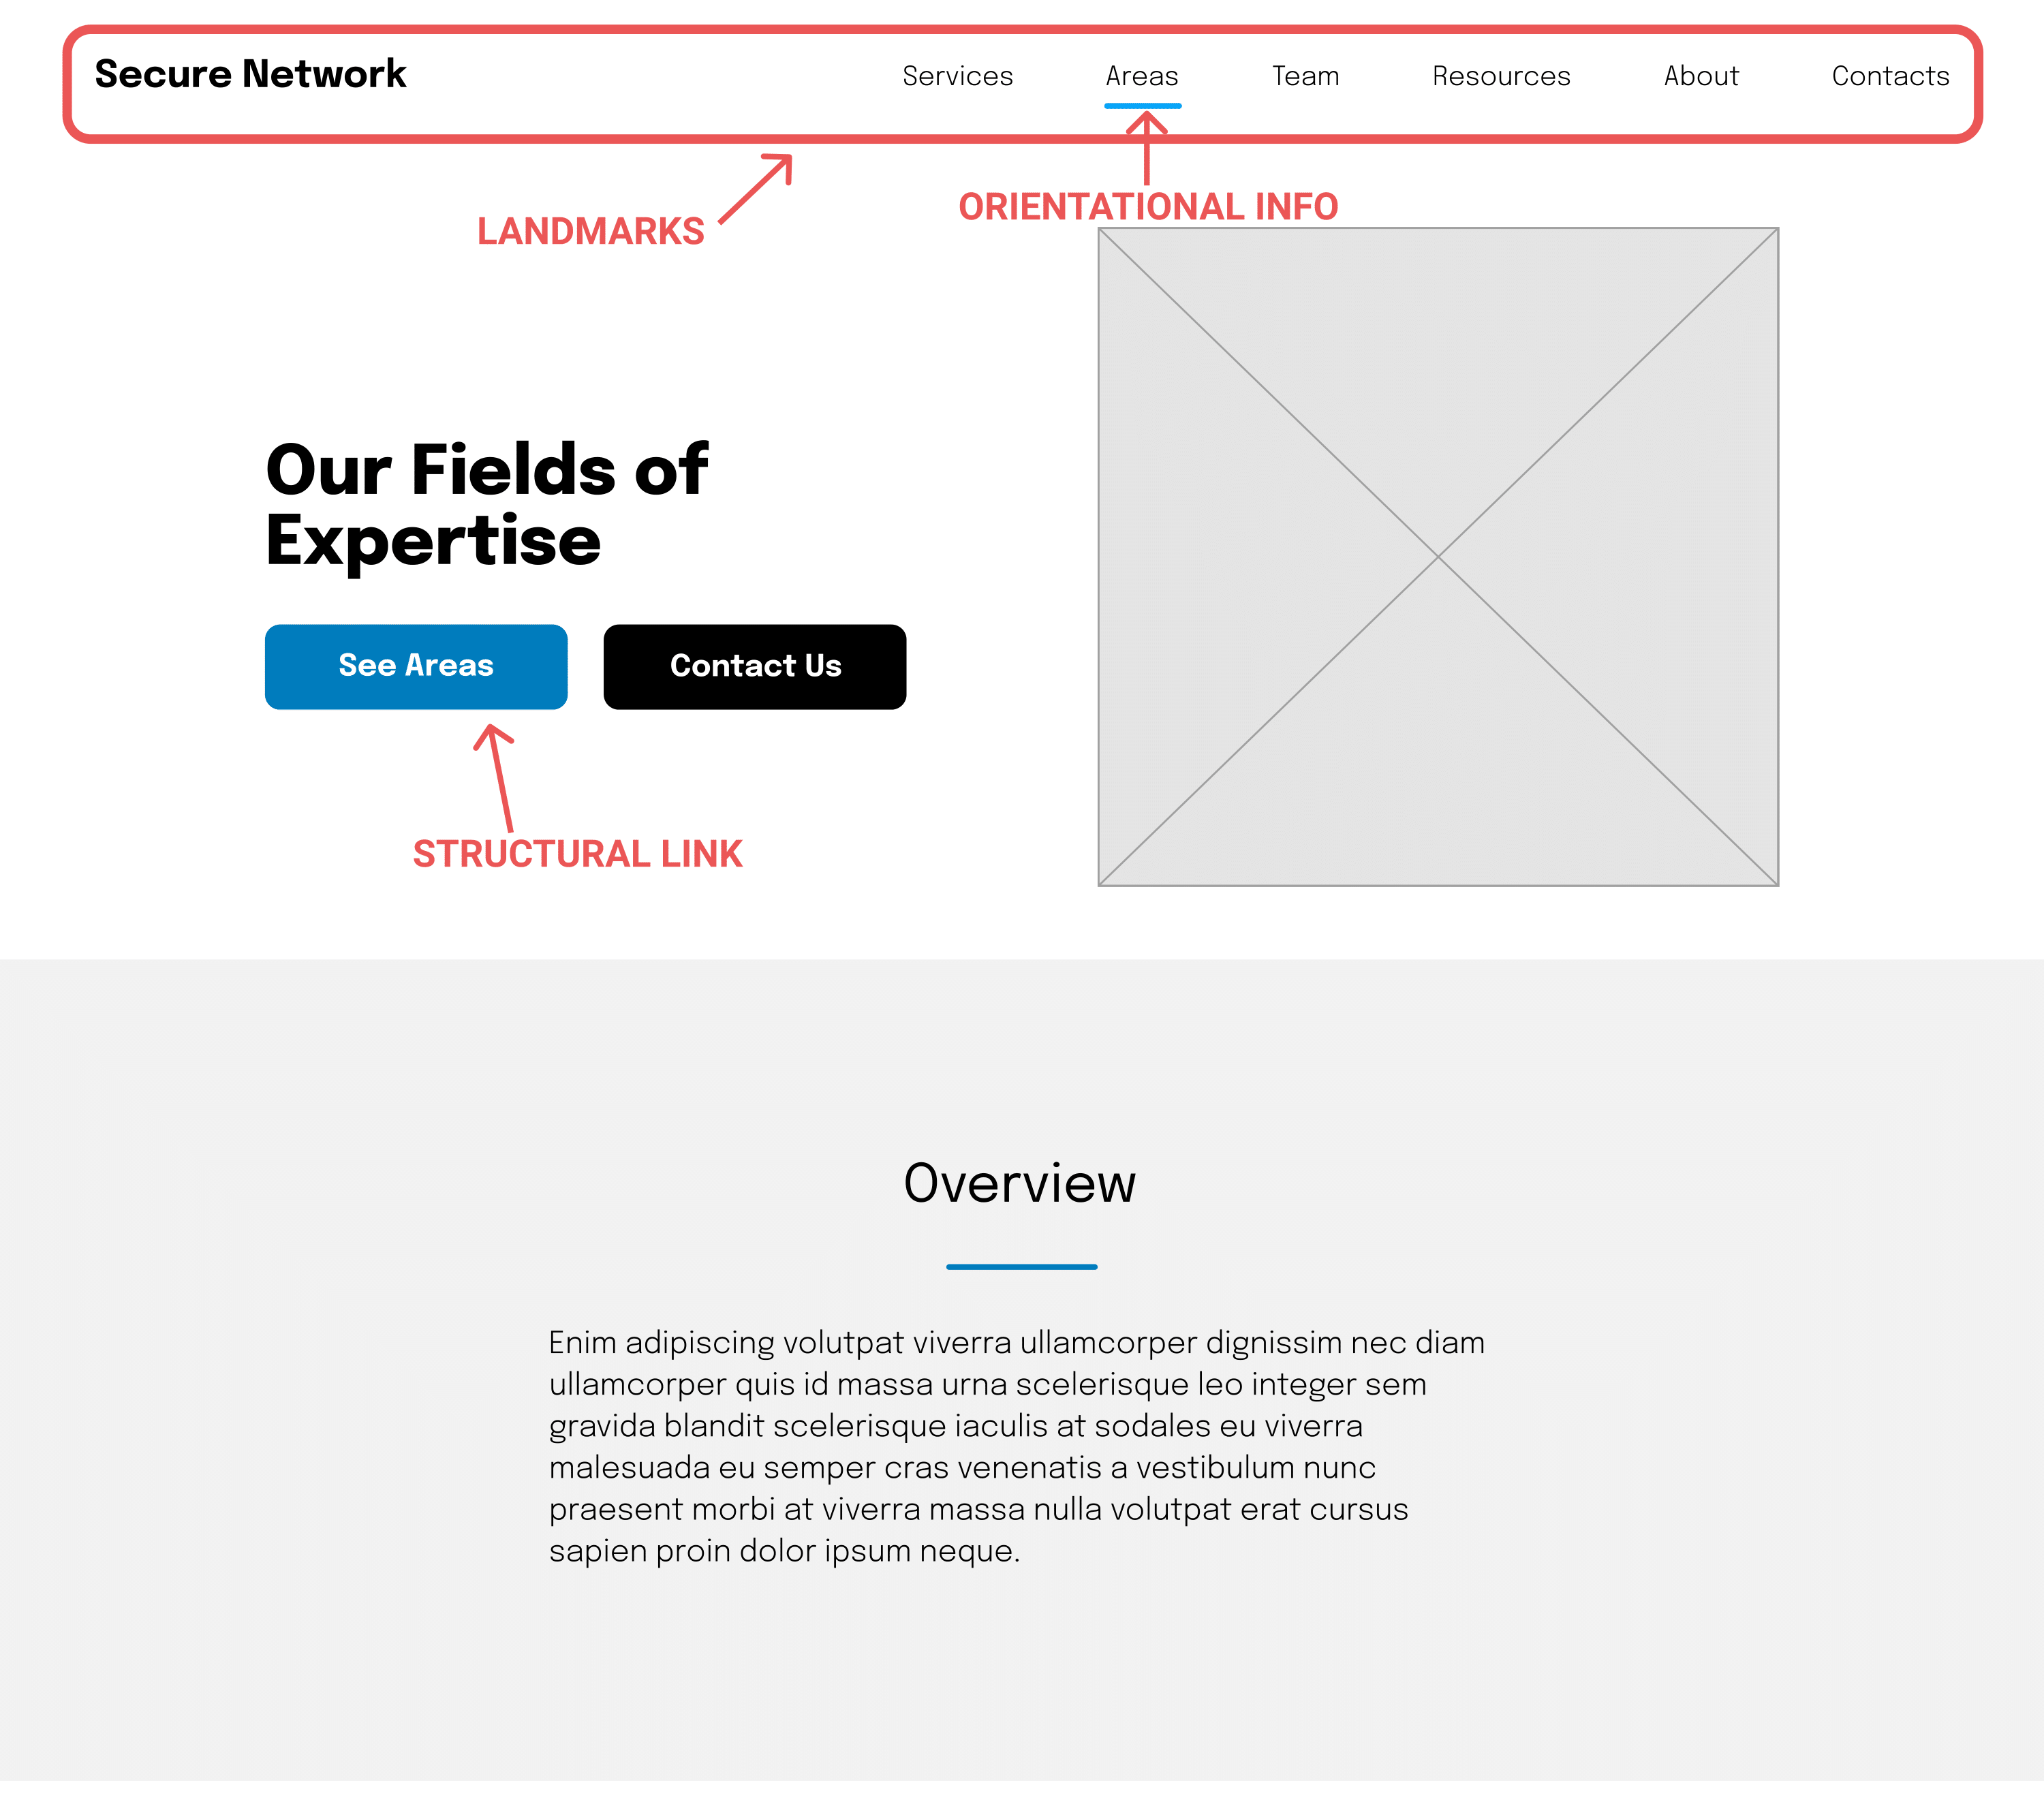
\includegraphics[width=0.45\textwidth]{low_fid_wireframes/all_areas/1.png}
	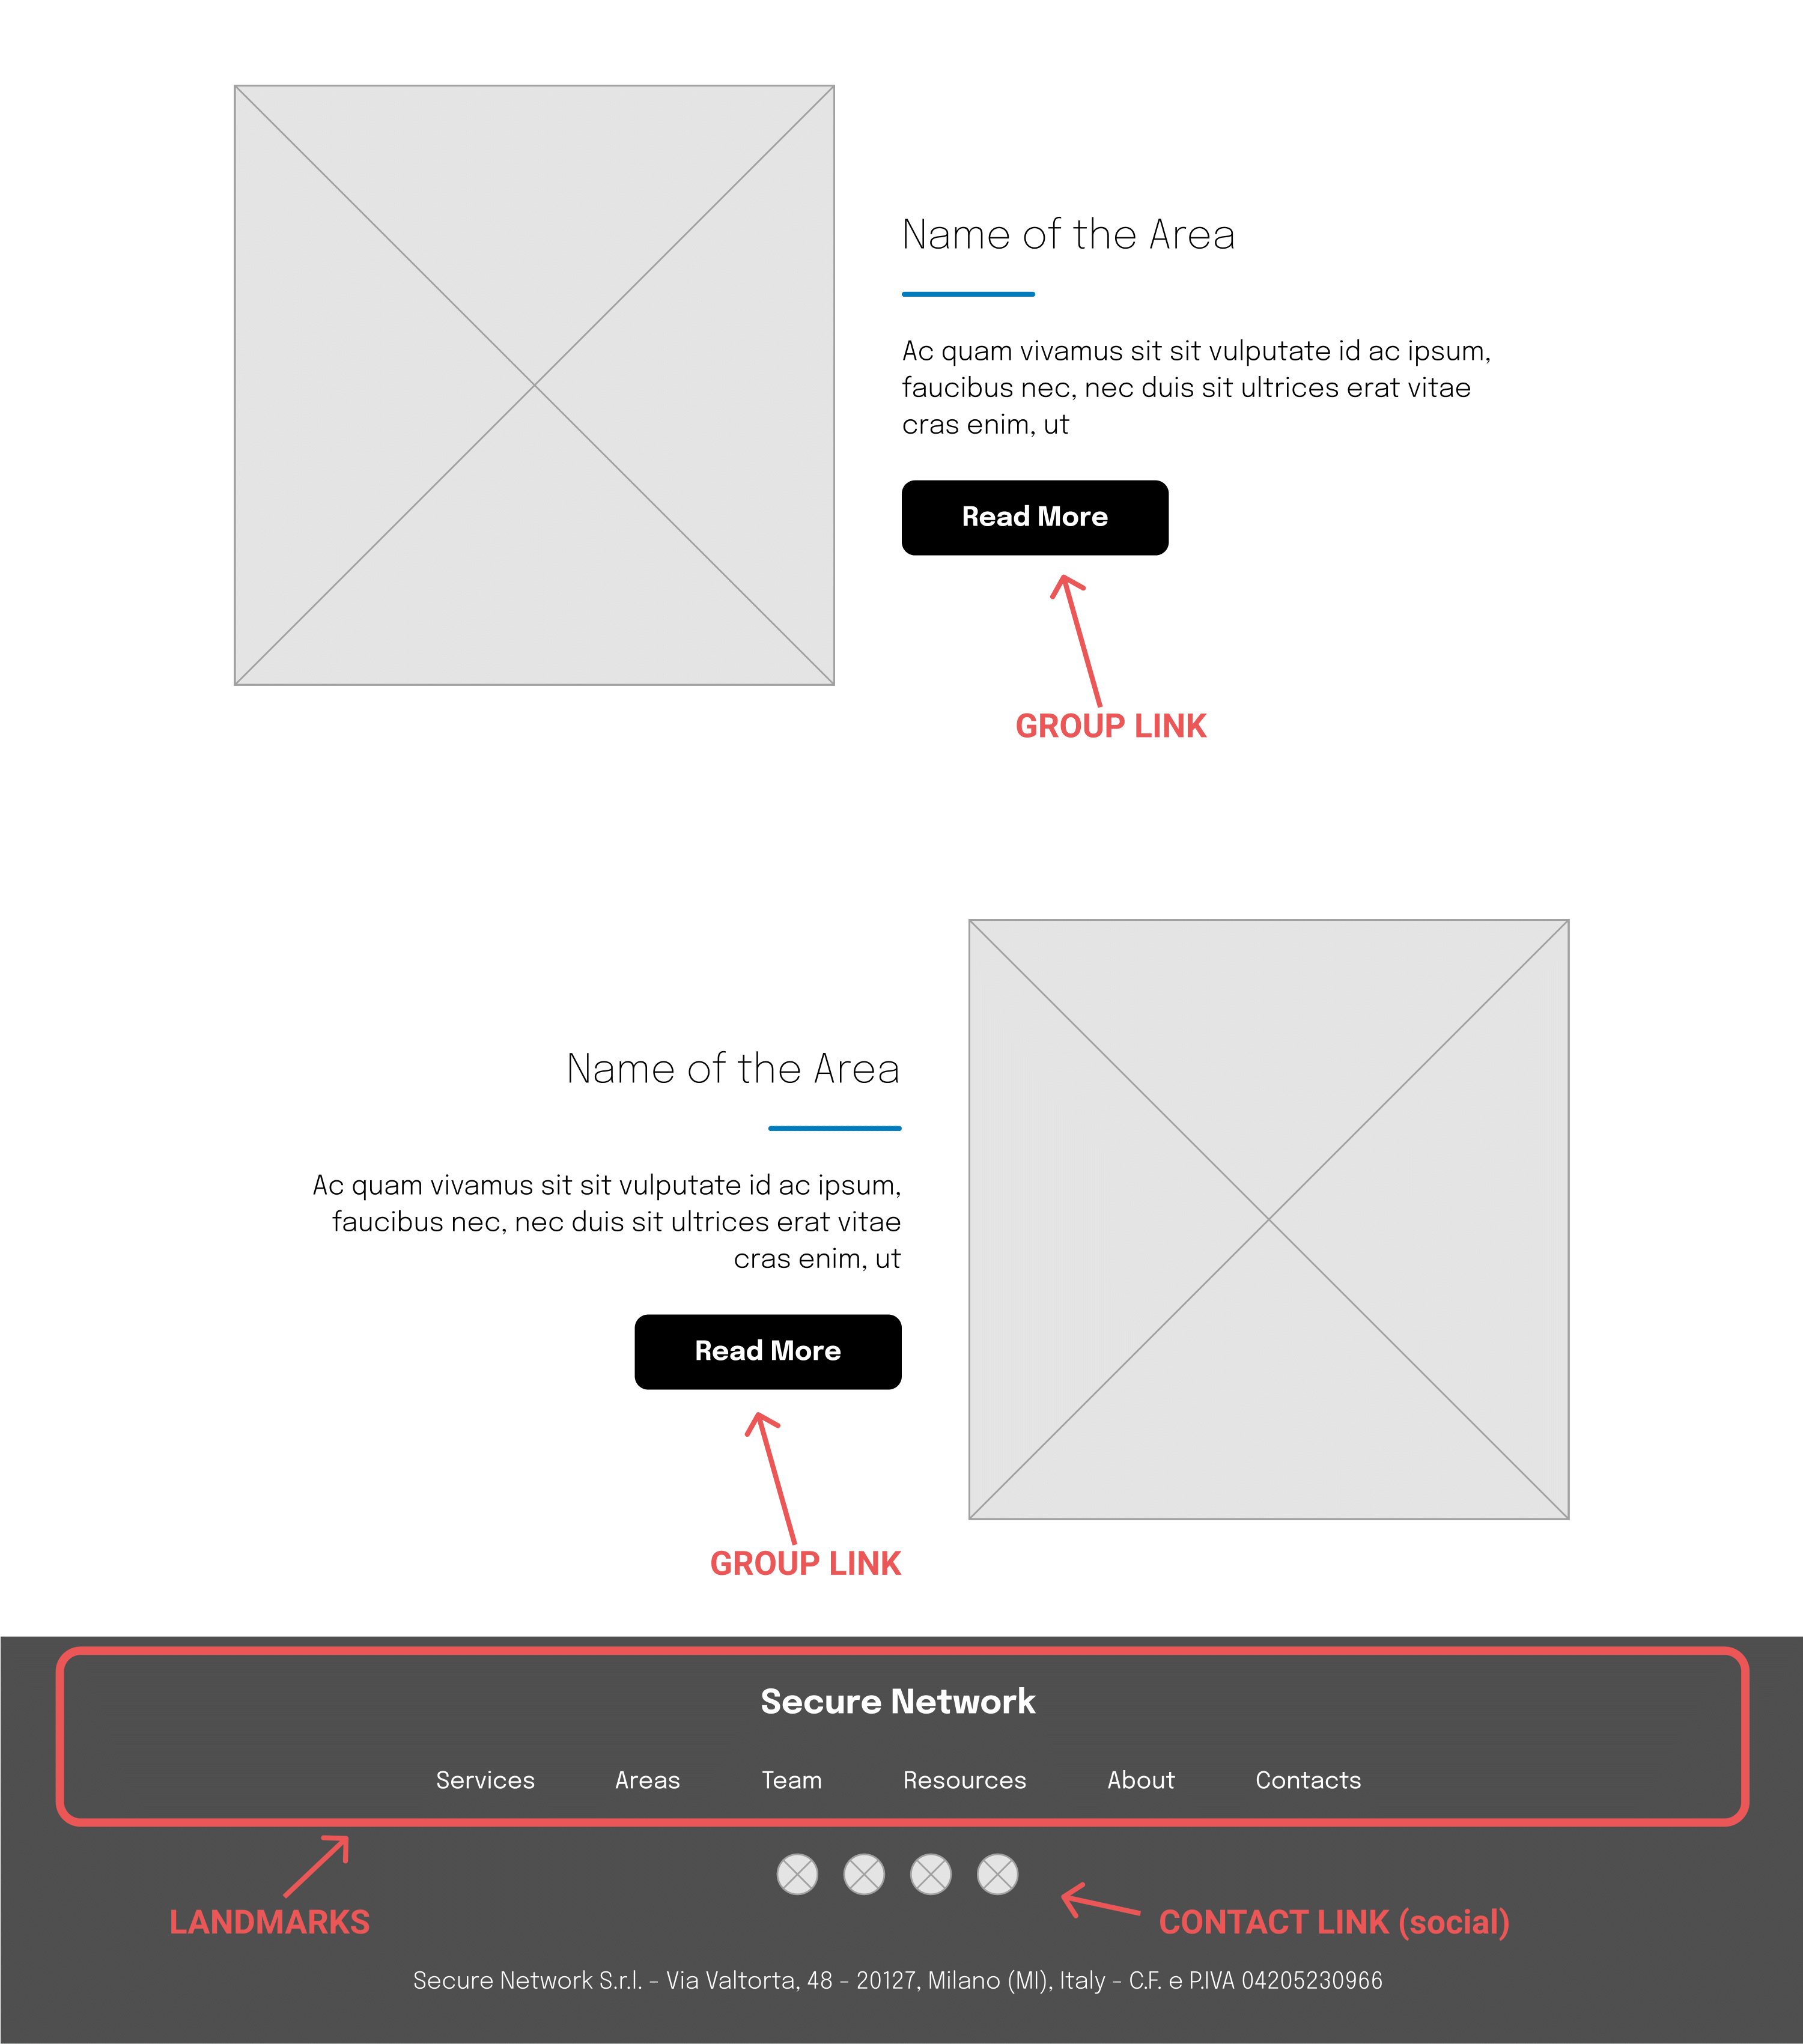
\includegraphics[width=0.45\textwidth]{low_fid_wireframes/all_areas/2.png}
	\caption{Commented wireframes for the Areas page.}
\end{figure}

\subsection{Group: Team}

\begin{figure}[H]
	\centering
	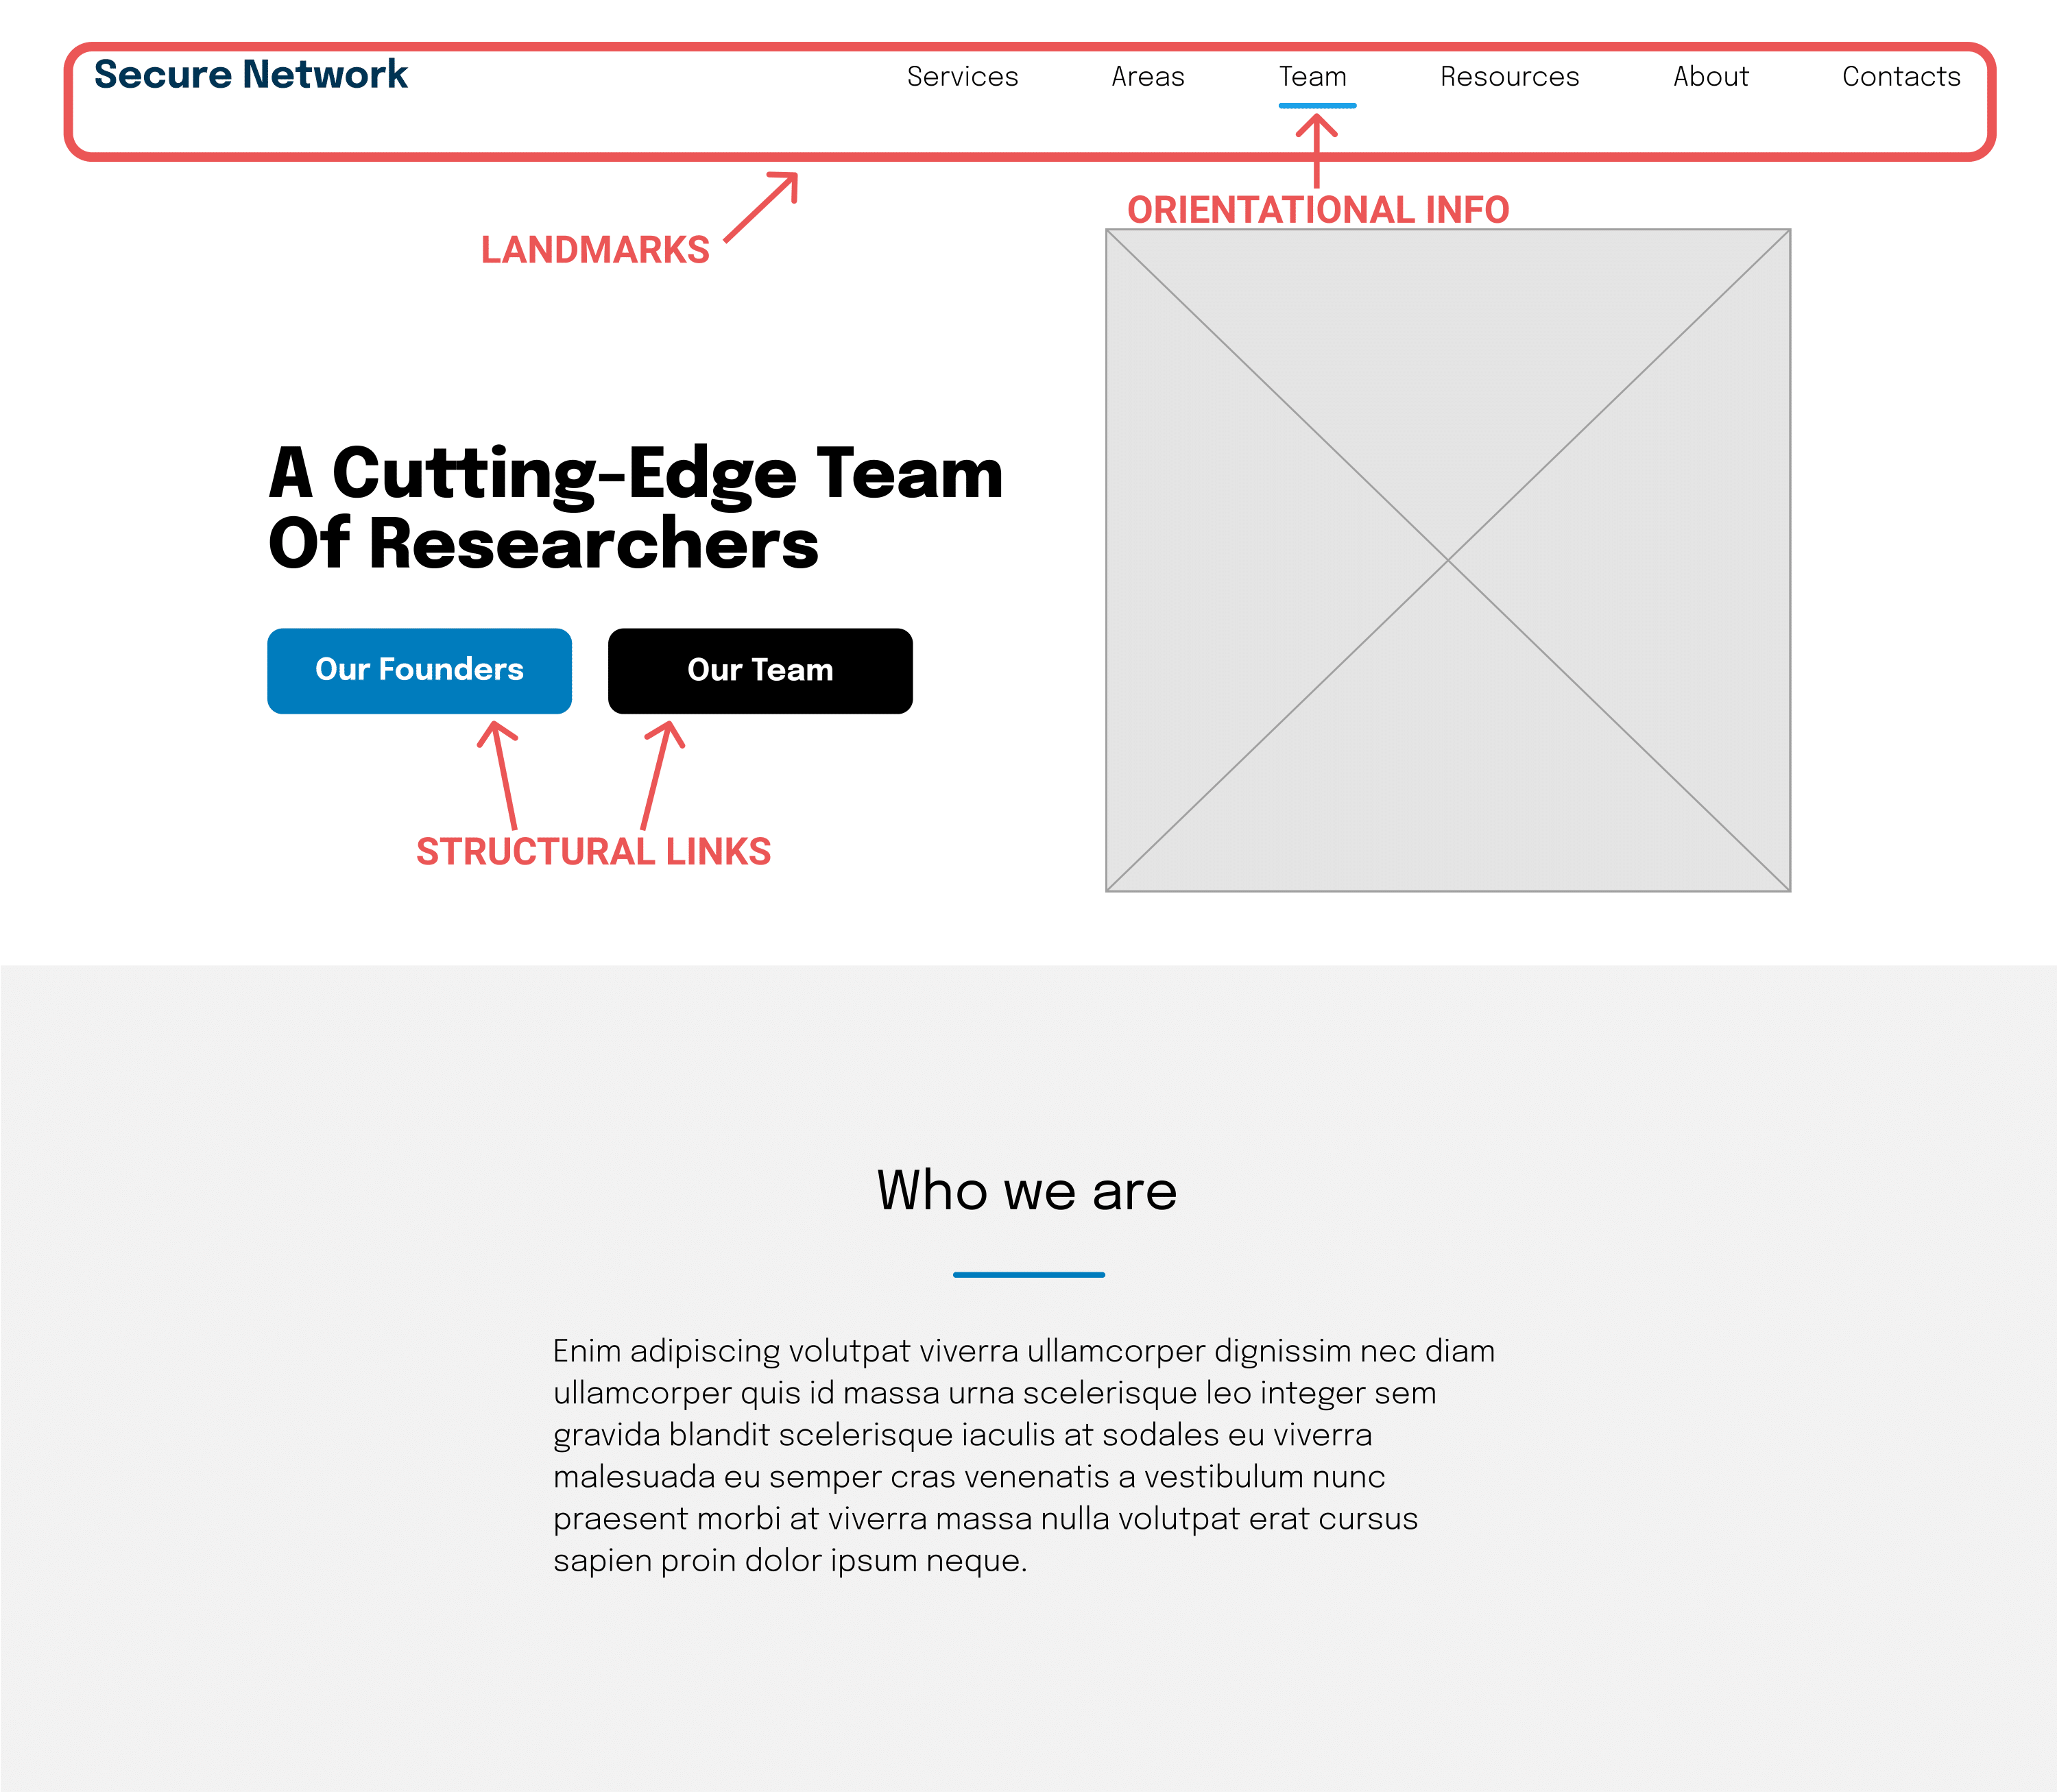
\includegraphics[width=0.45\textwidth]{low_fid_wireframes/team/1.png}
	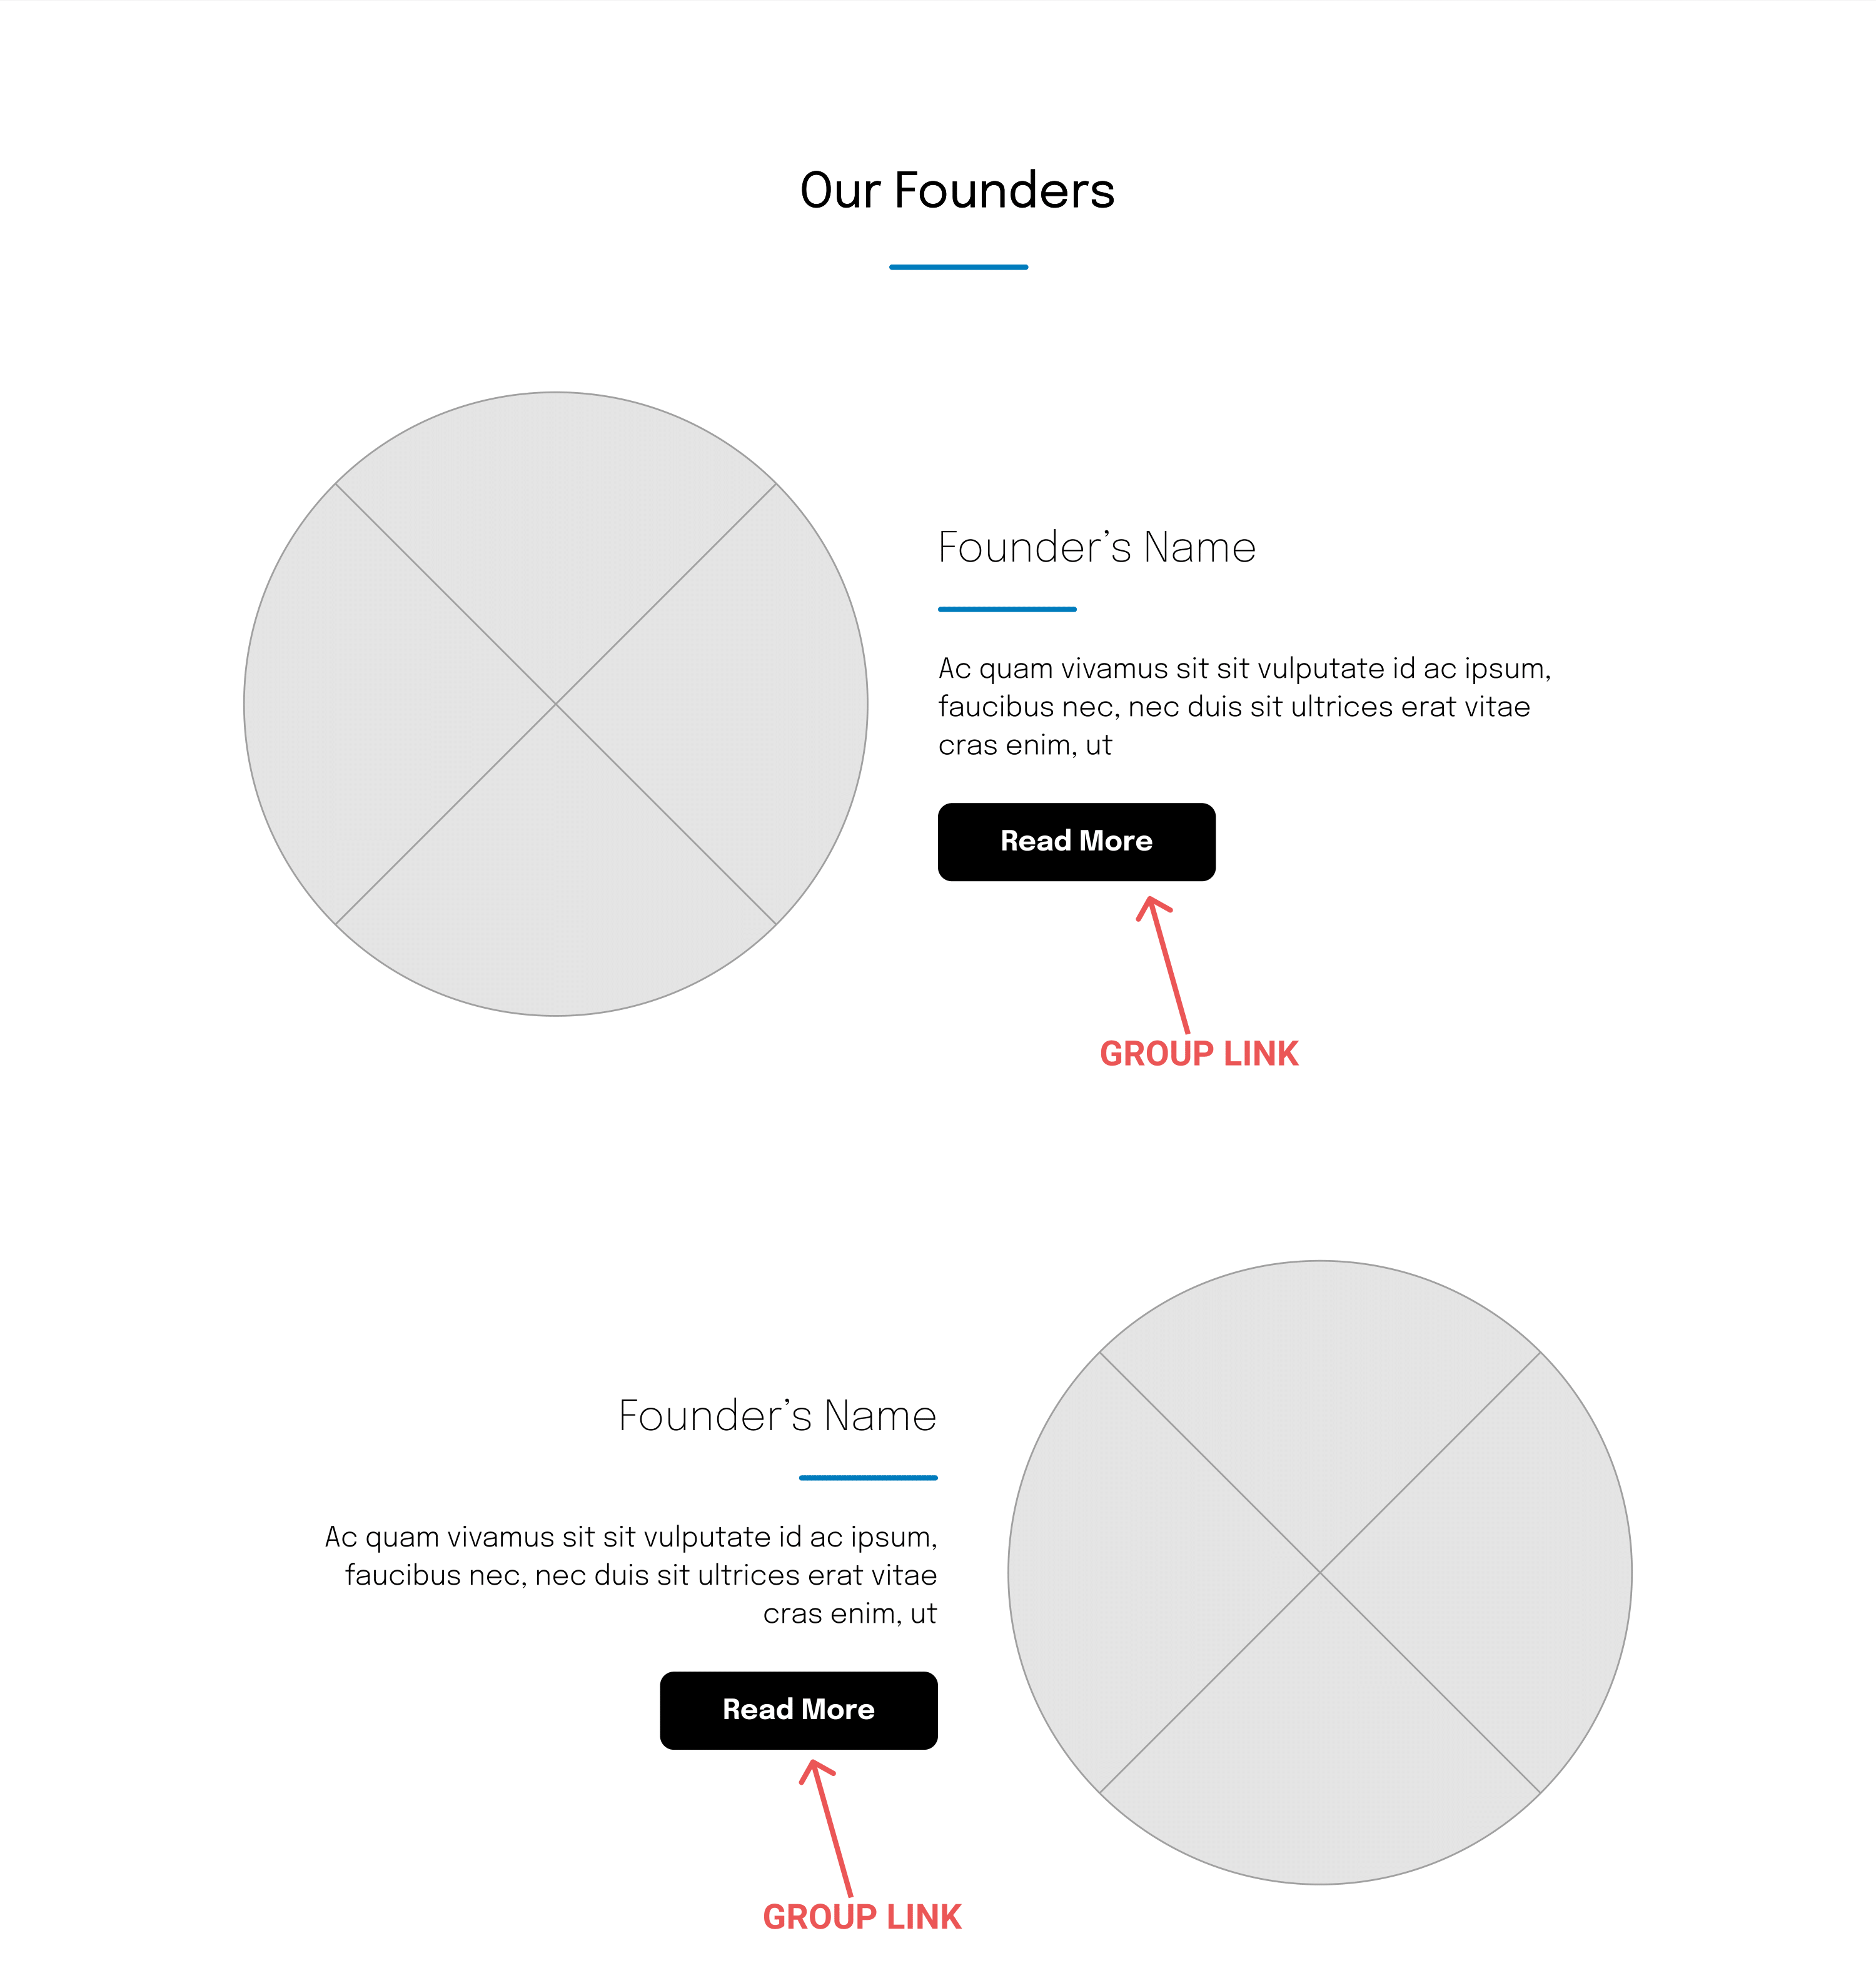
\includegraphics[width=0.45\textwidth]{low_fid_wireframes/team/2.png}
	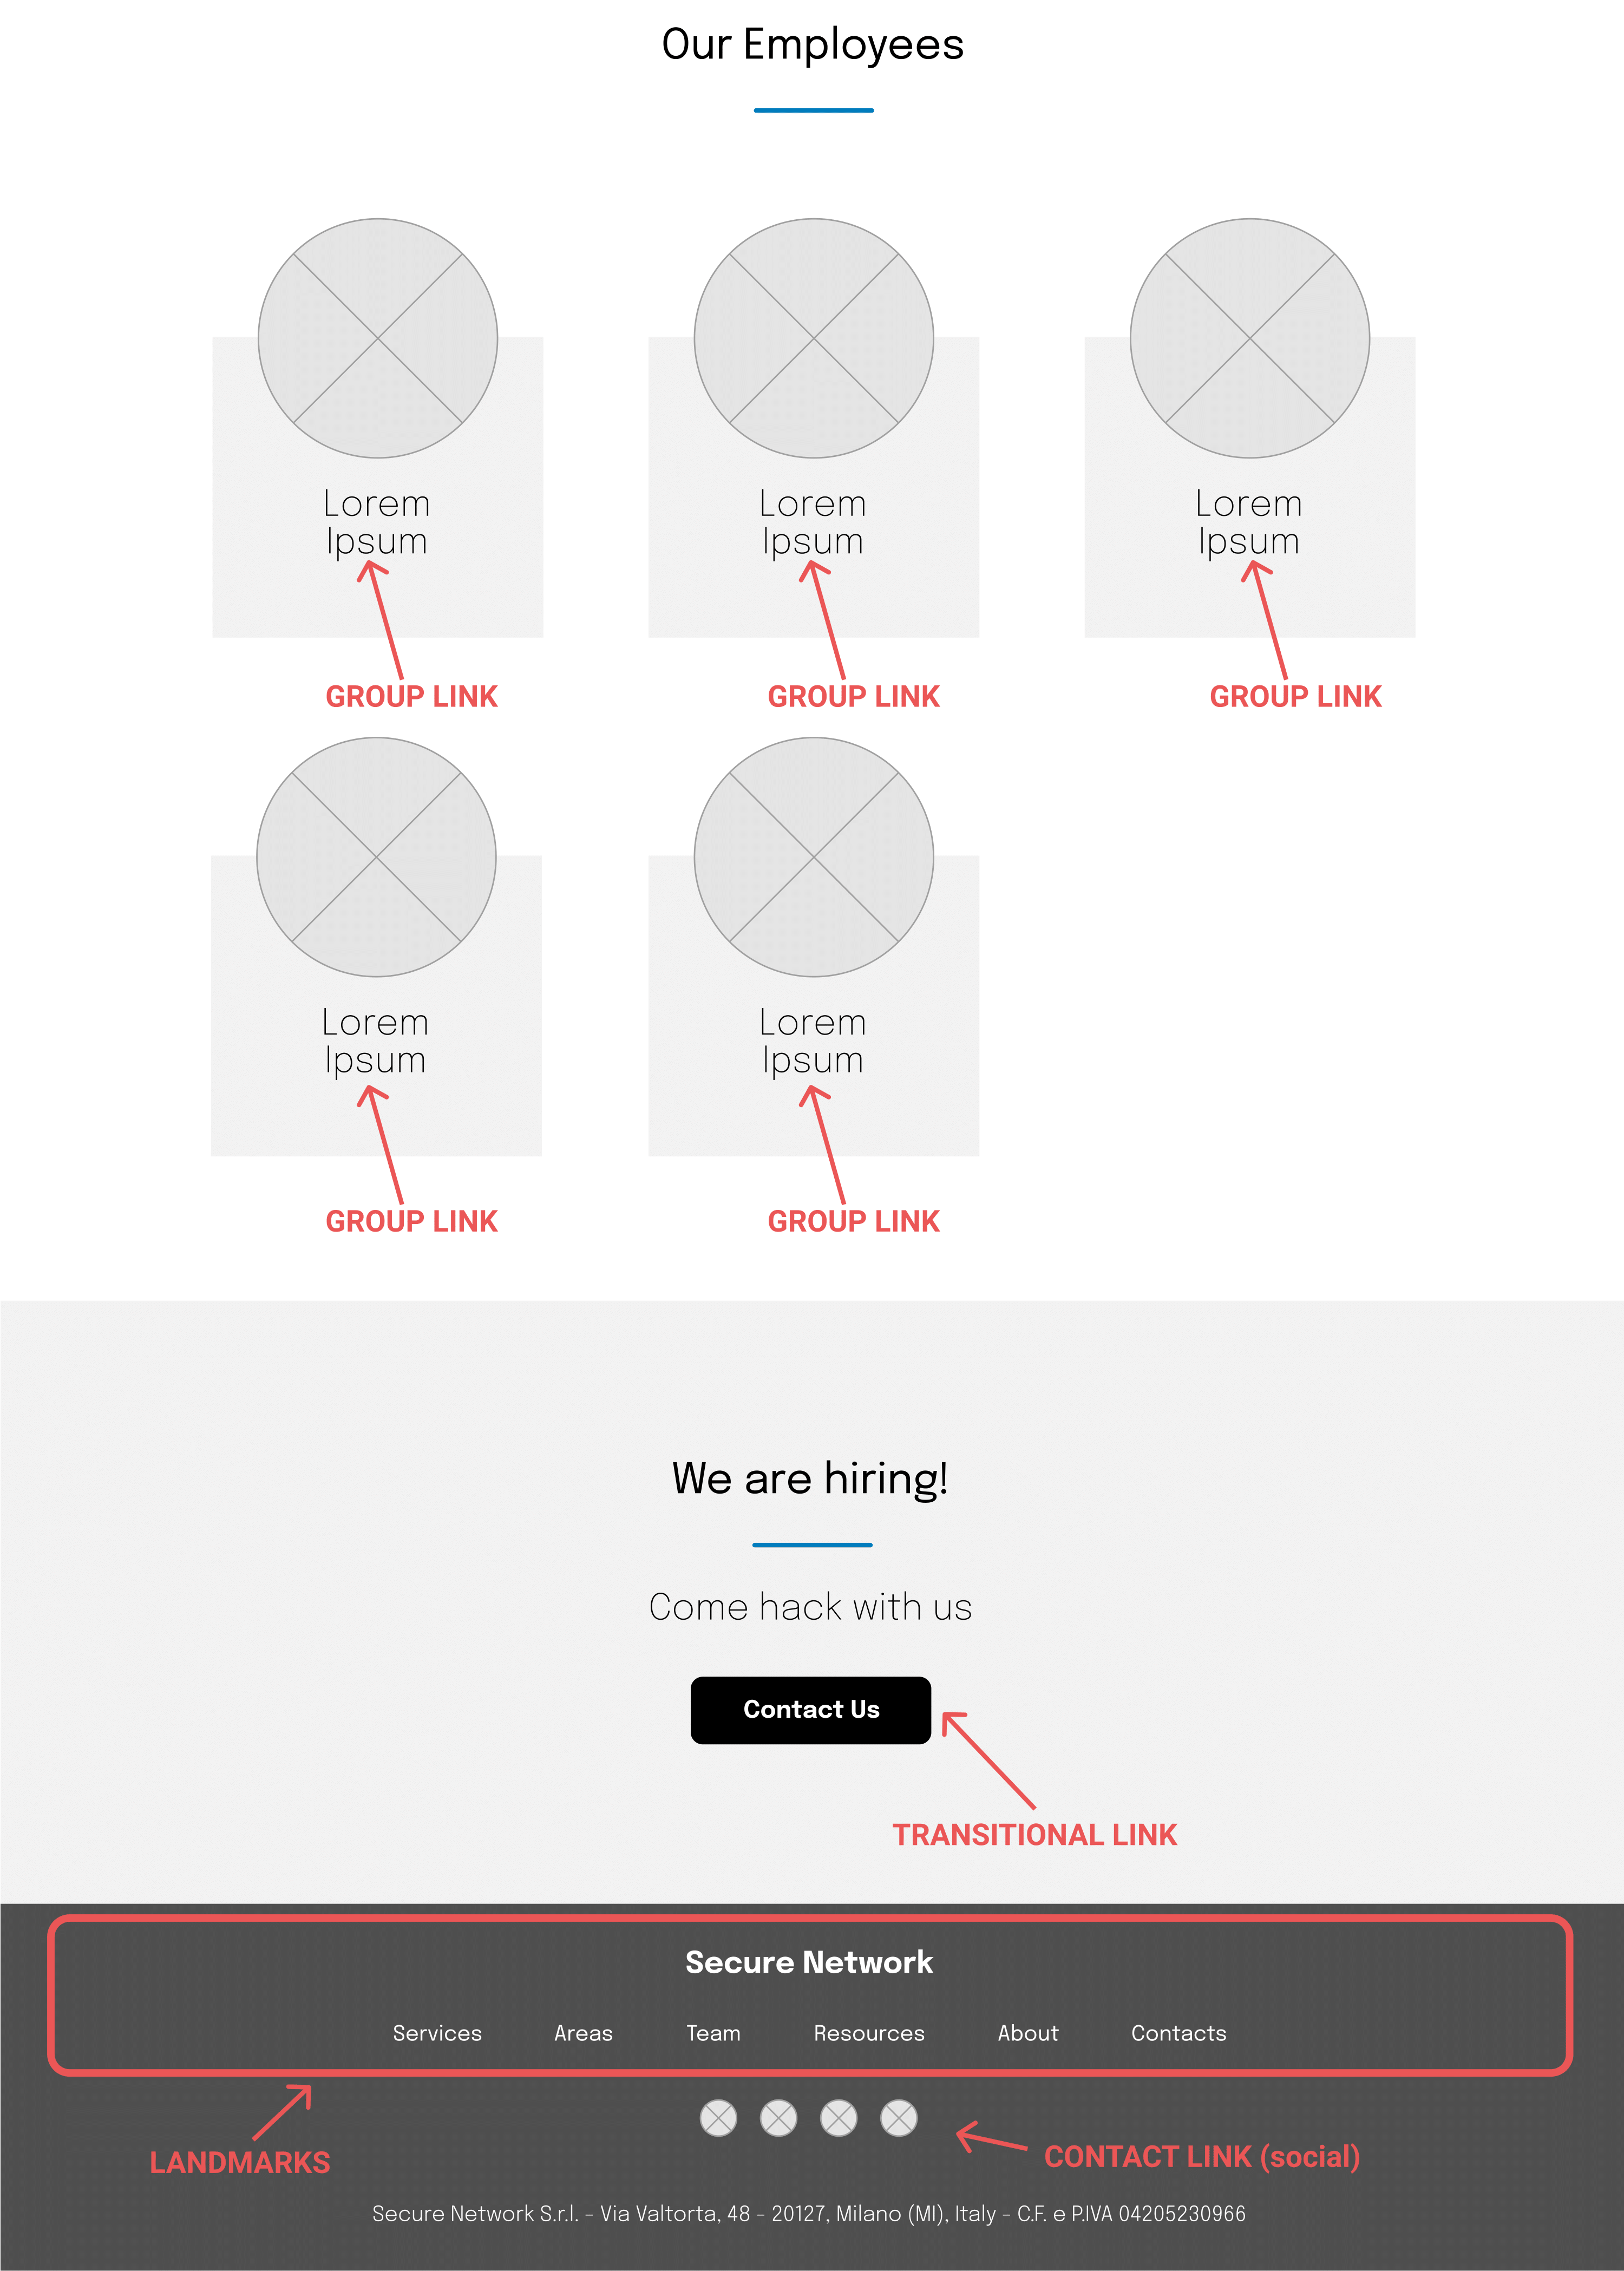
\includegraphics[width=0.45\textwidth]{low_fid_wireframes/team/3.png}
	\caption{Commented wireframes for the Team page.}
\end{figure}

\subsection{Group: Resources}

\begin{figure}[H]
	\centering
	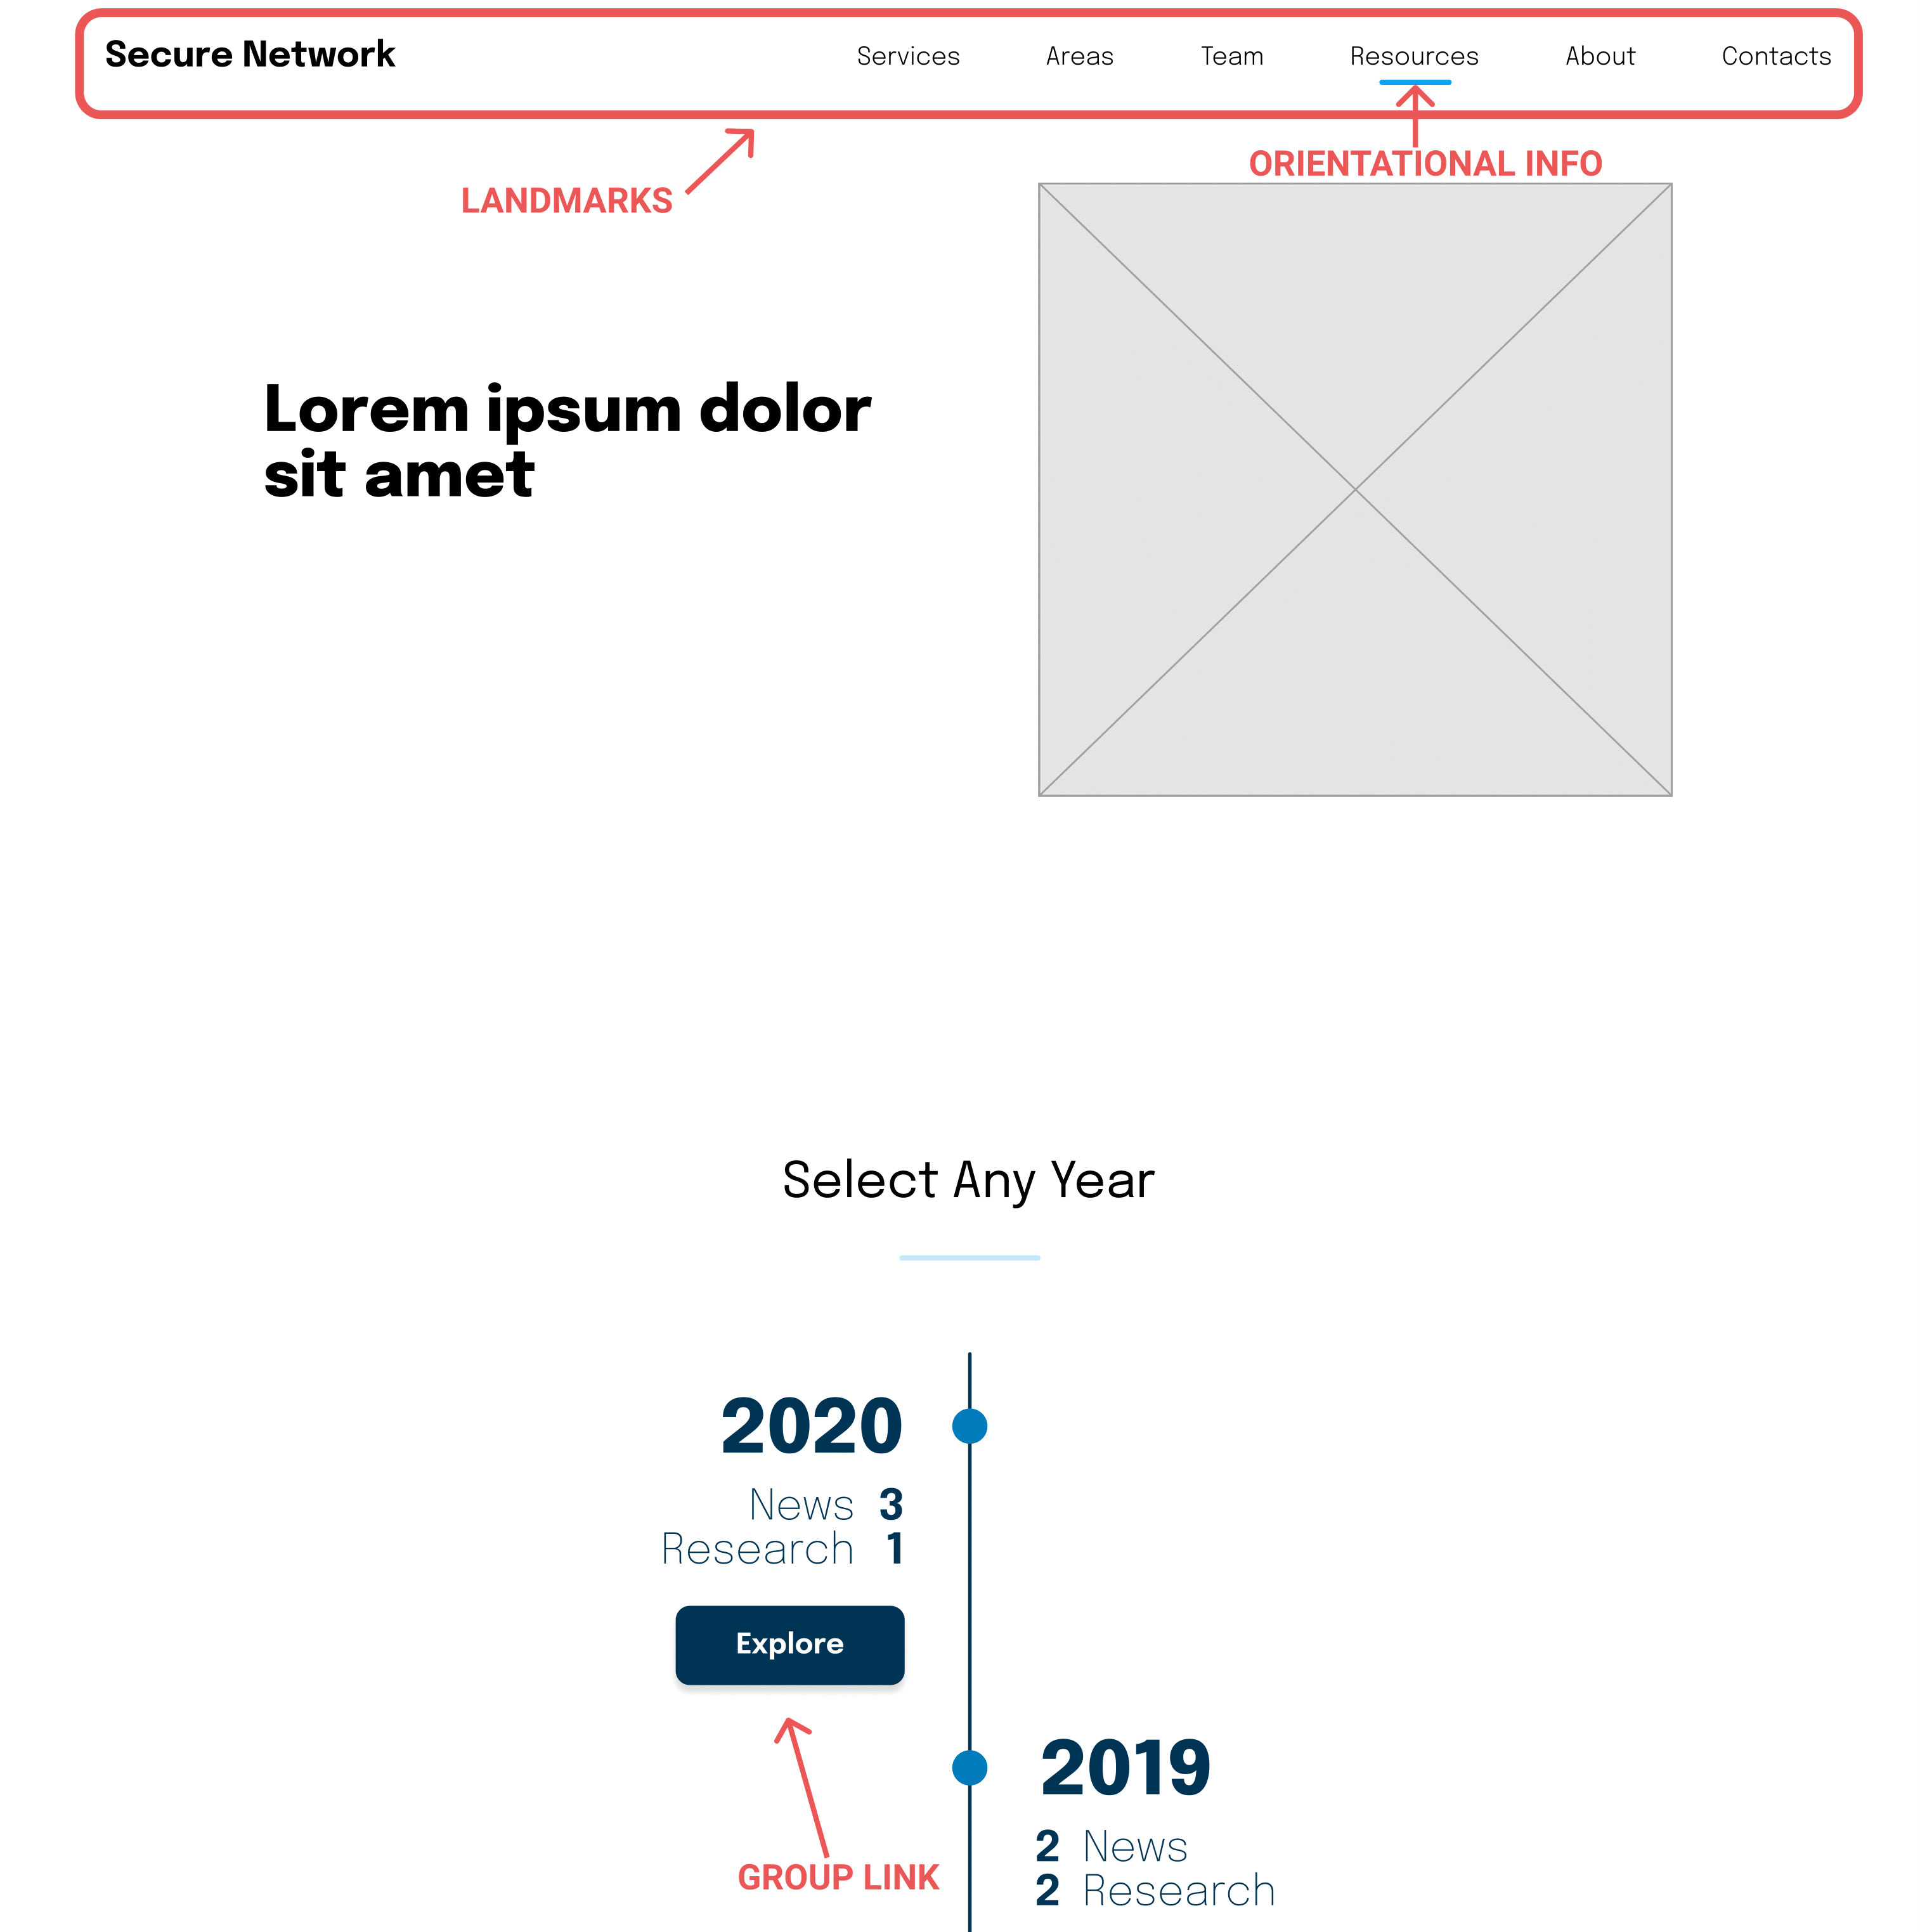
\includegraphics[width=0.45\textwidth]{low_fid_wireframes/all_resources/1.png}
	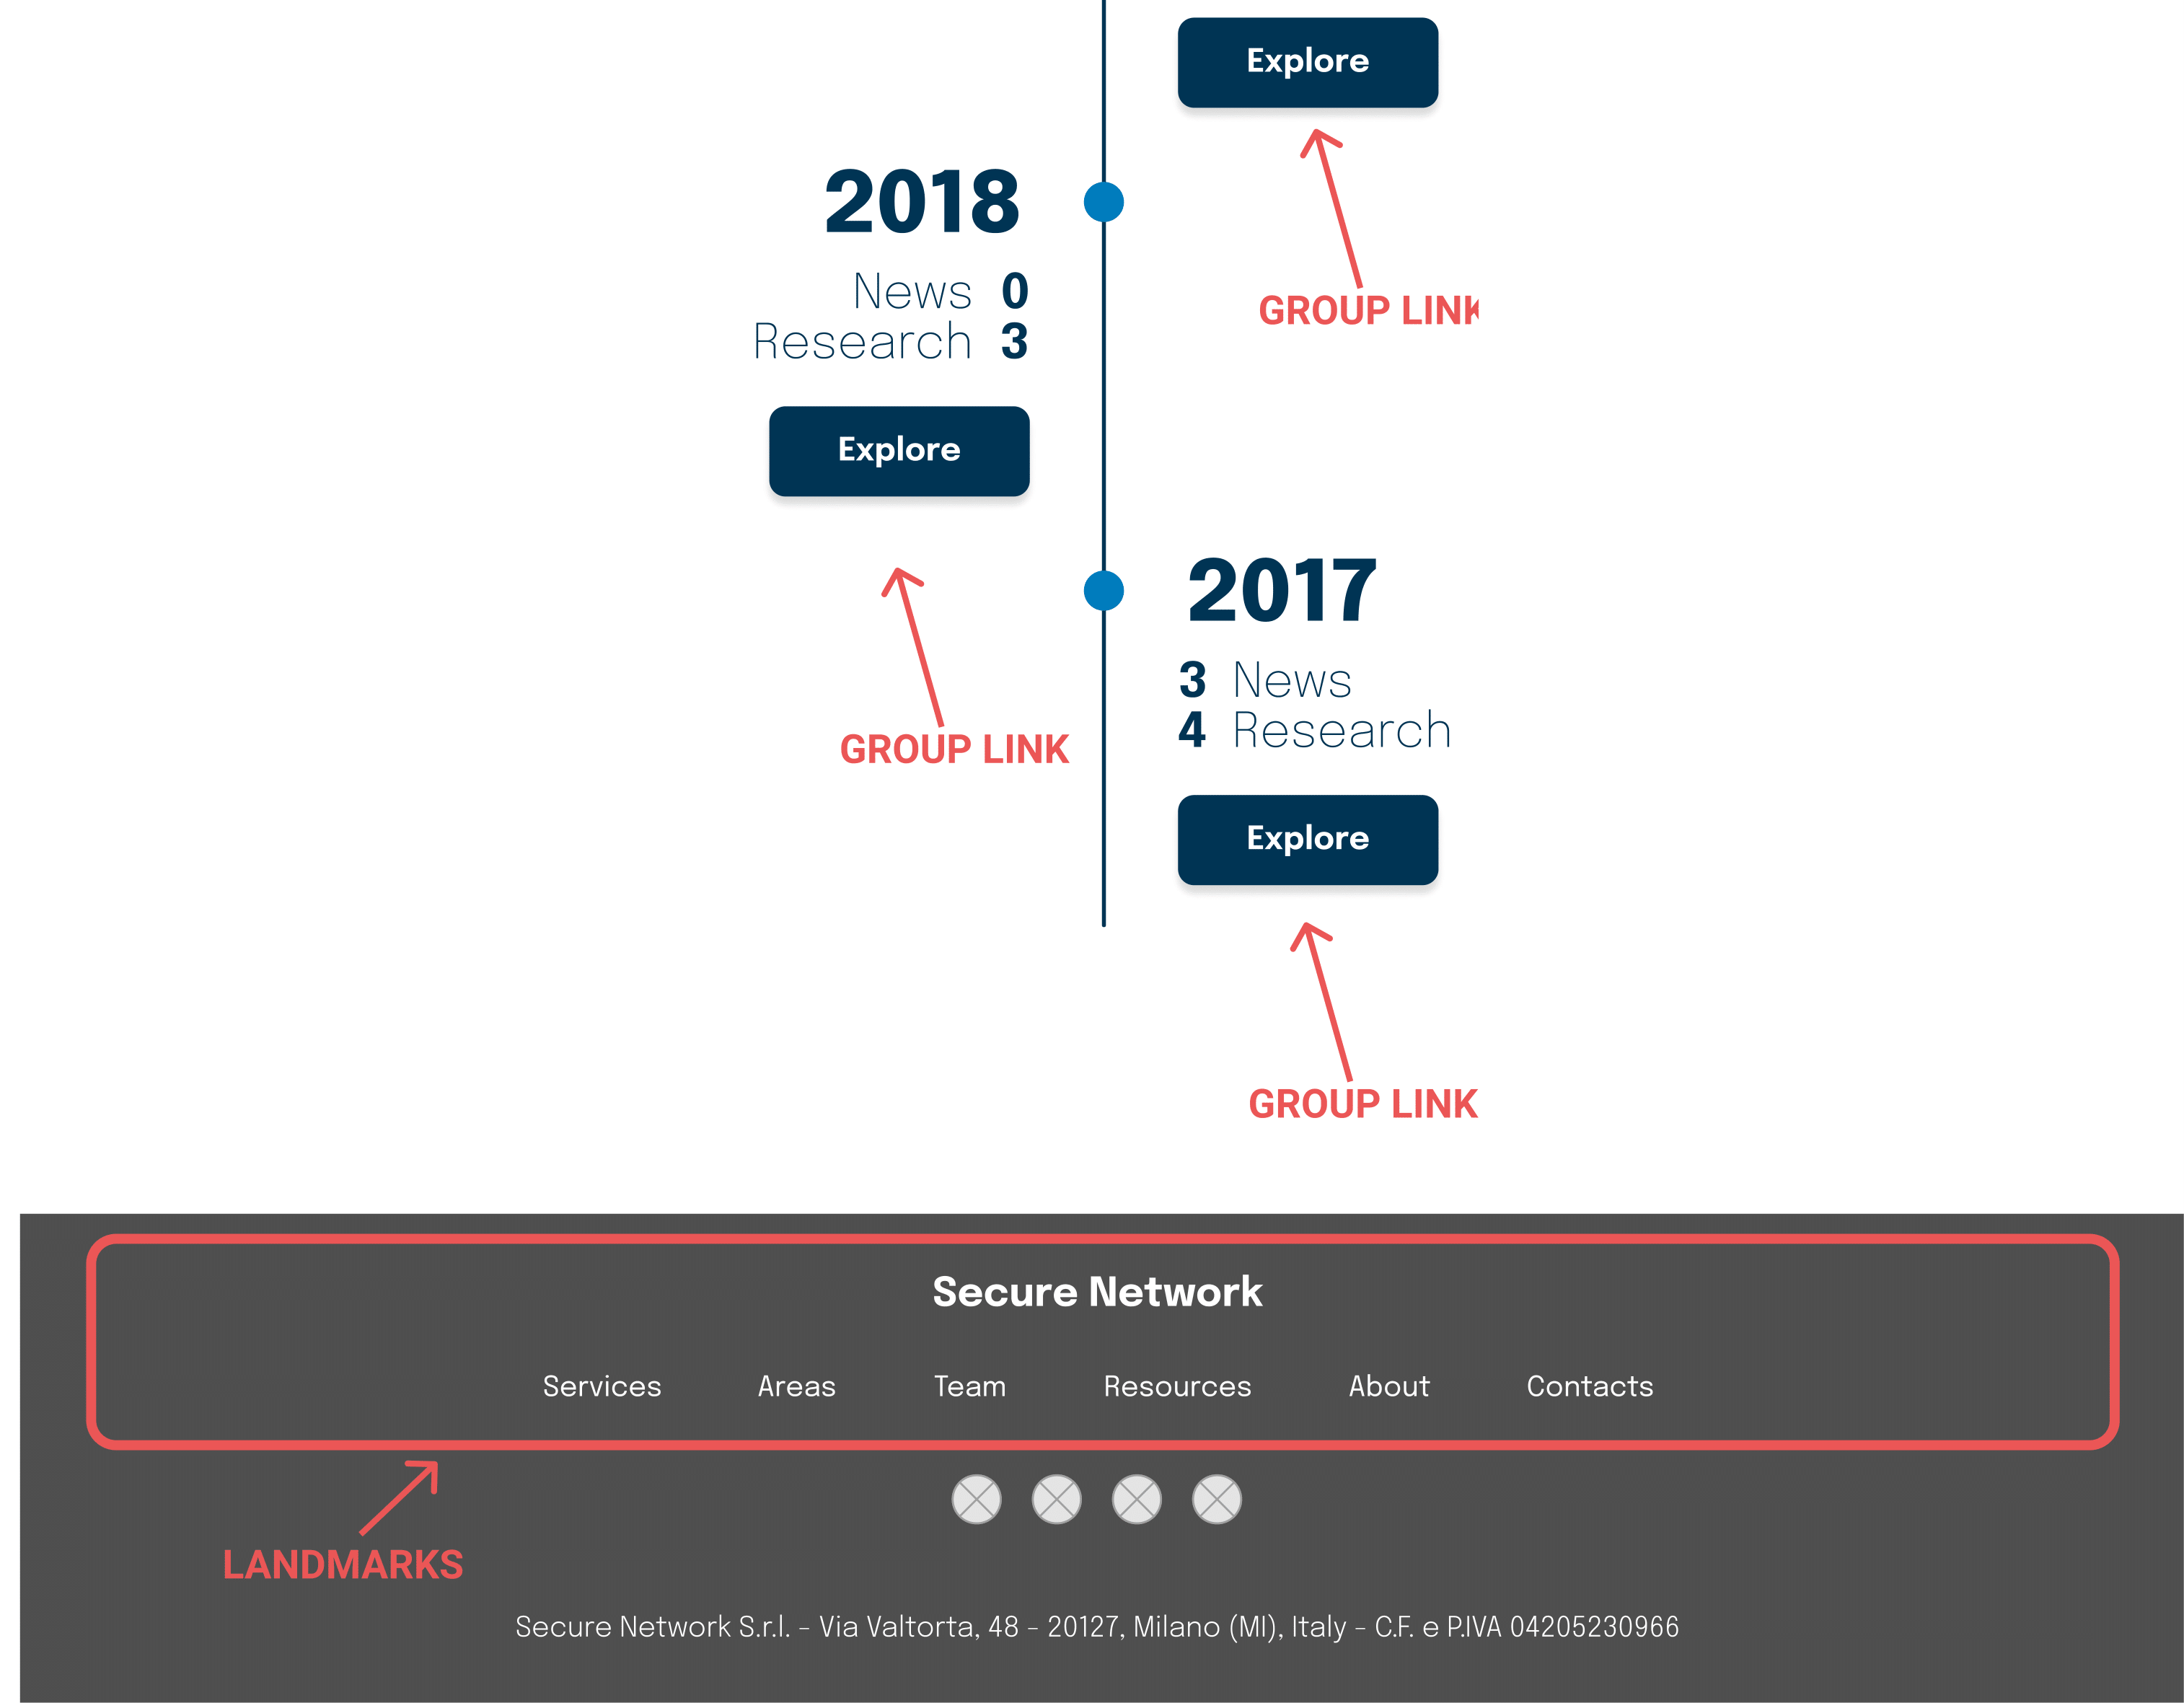
\includegraphics[width=0.45\textwidth]{low_fid_wireframes/all_resources/2.png}
	\caption{Commented wireframes for the Resources page.}
\end{figure}

\section{High-Fidelity Screenshots}

\subsection{Home Page}

\begin{figure}[H]
	\centering
	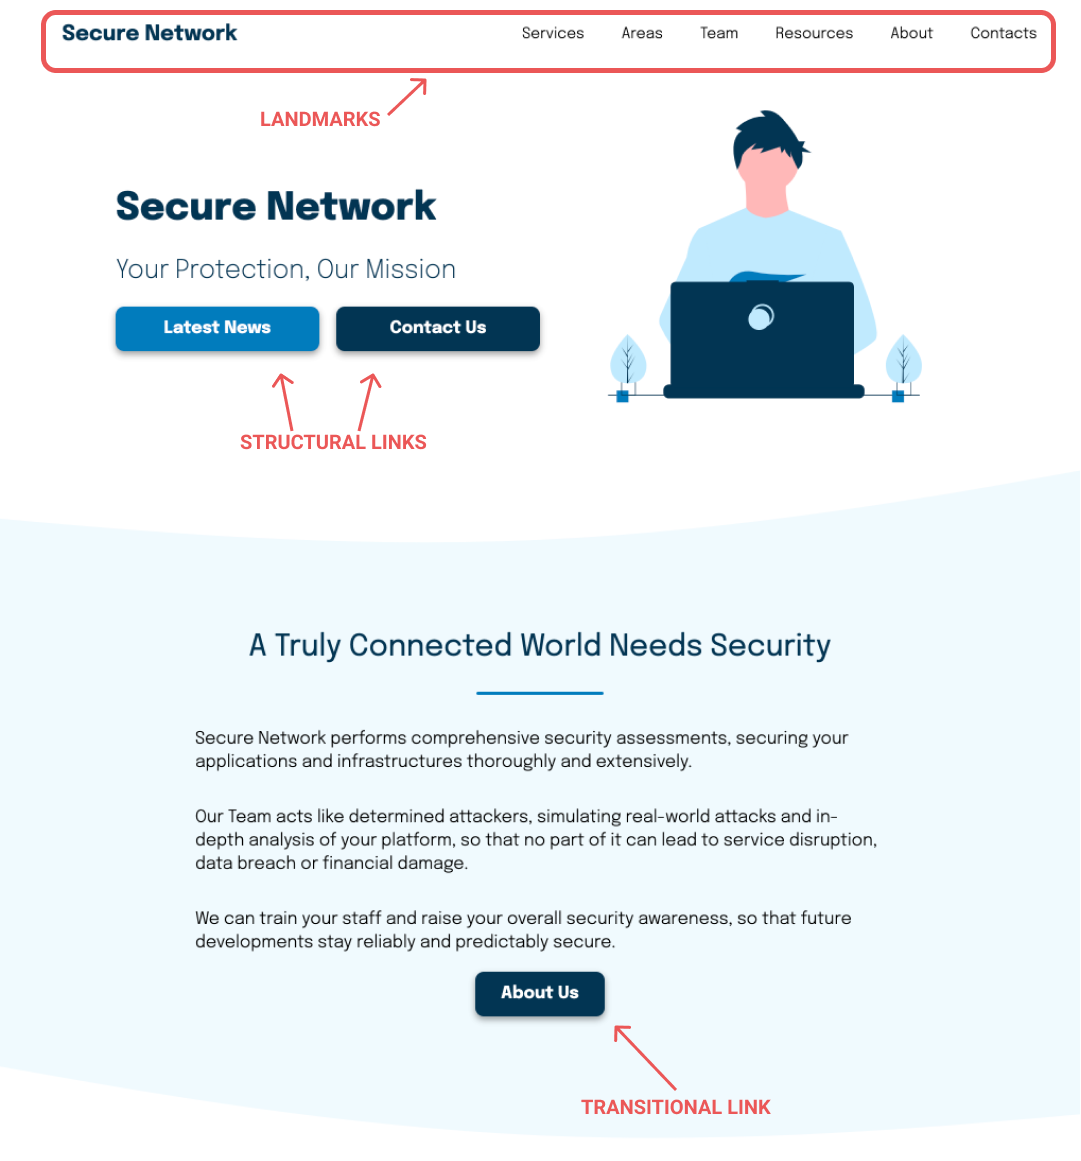
\includegraphics[width=0.45\textwidth]{high_fid_wireframes/home/1.png}
	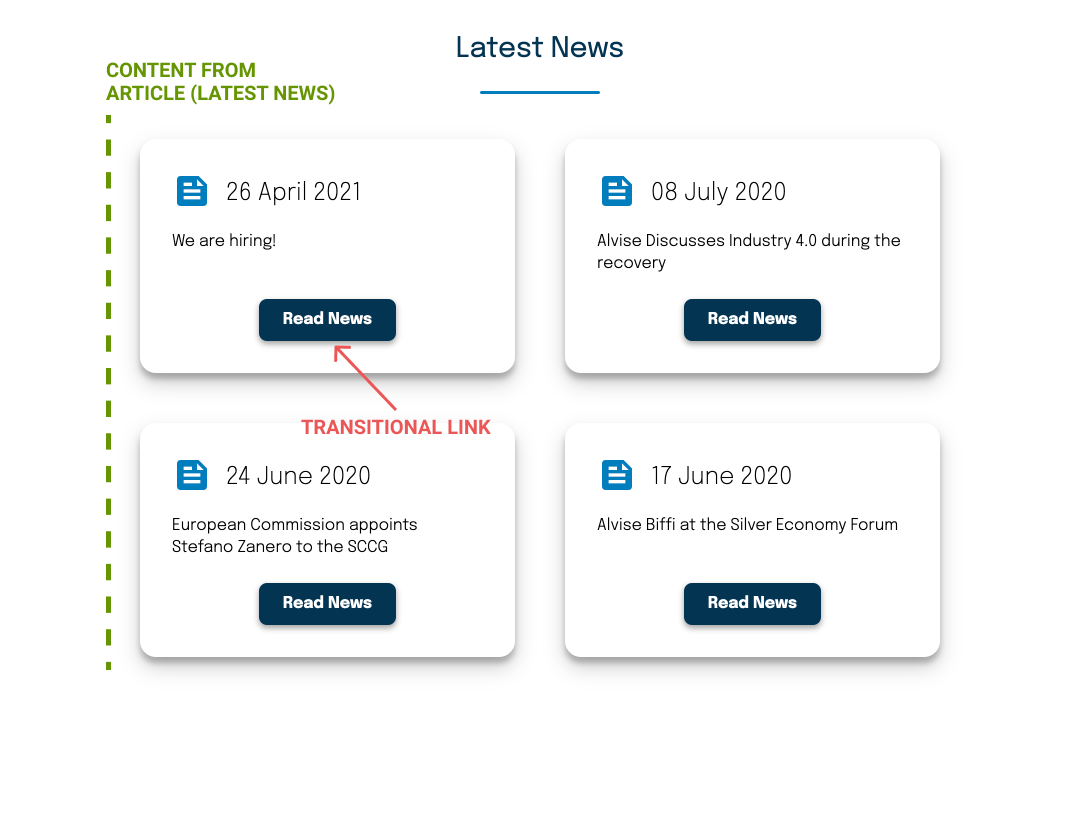
\includegraphics[width=0.45\textwidth]{high_fid_wireframes/home/2.png}
	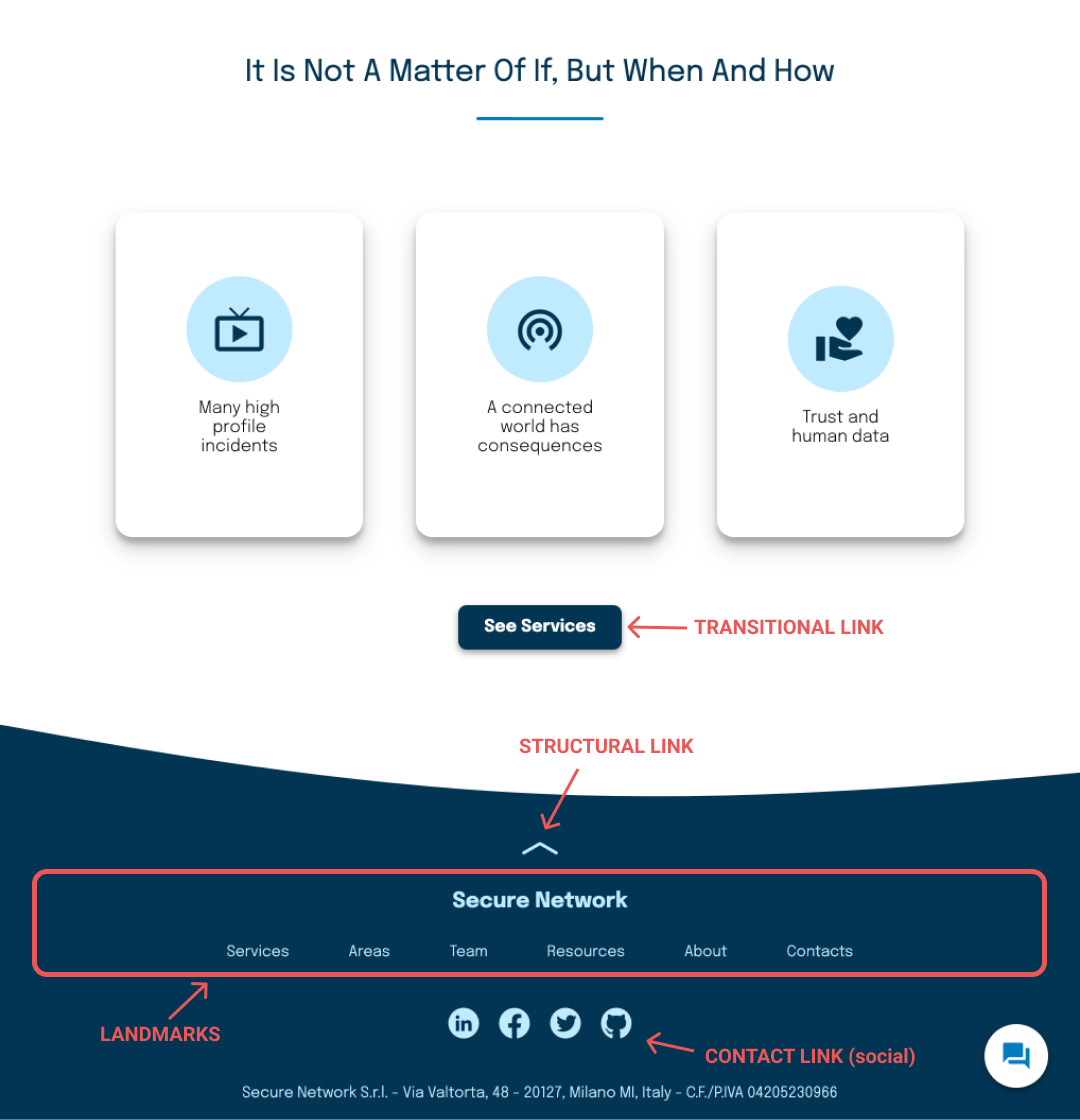
\includegraphics[width=0.45\textwidth]{high_fid_wireframes/home/3.png}
	\caption{Commented screenshots for the Home page.}
\end{figure}

\subsection{Topic: Contacts}

\begin{figure}[H]
	\centering
	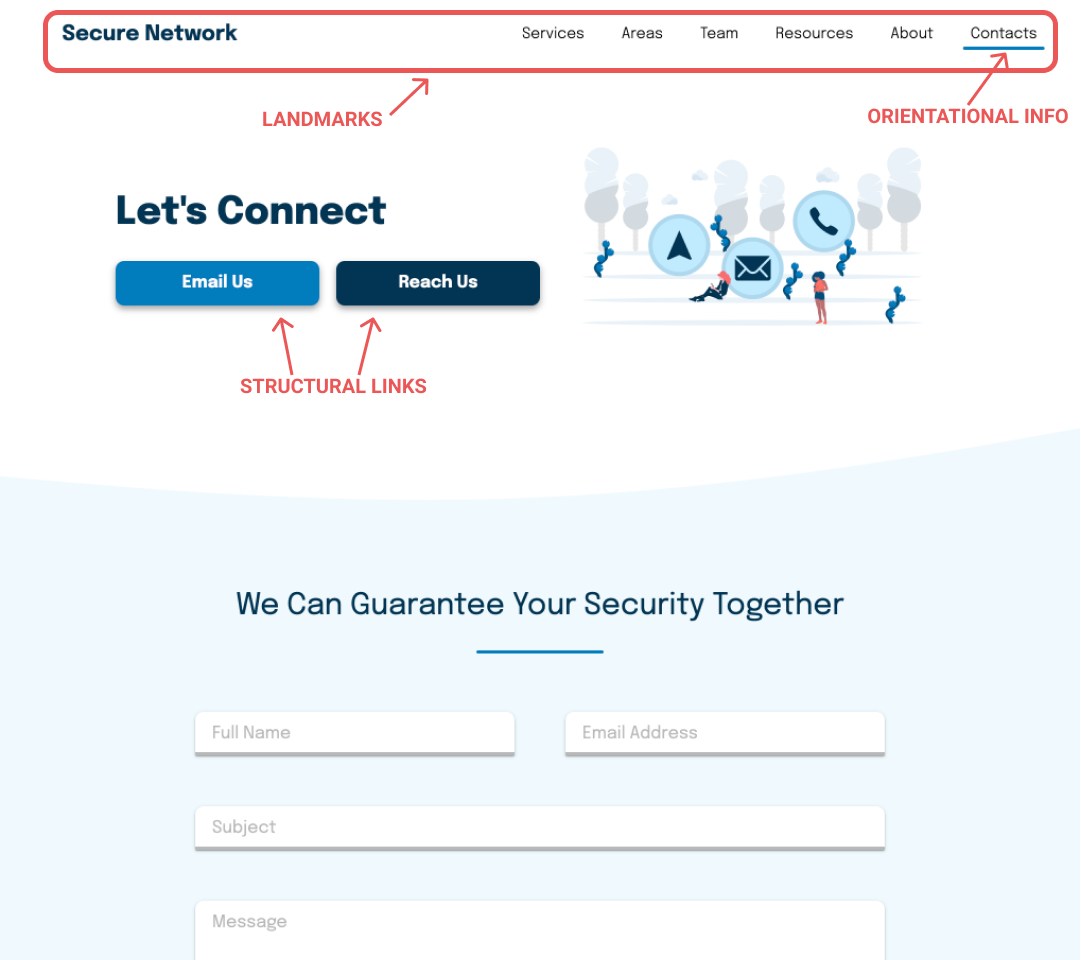
\includegraphics[width=0.45\textwidth]{high_fid_wireframes/contacts/1.png}
	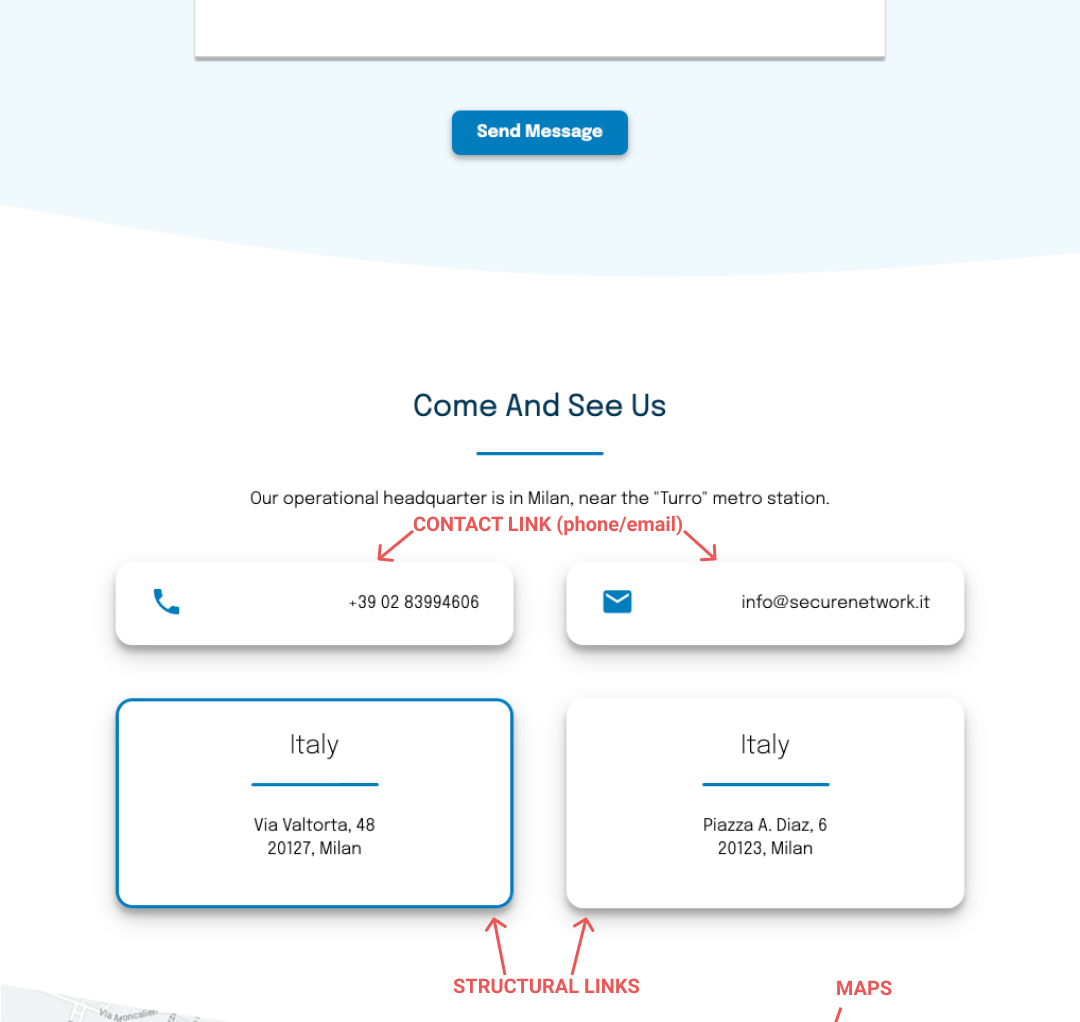
\includegraphics[width=0.45\textwidth]{high_fid_wireframes/contacts/2.png}
	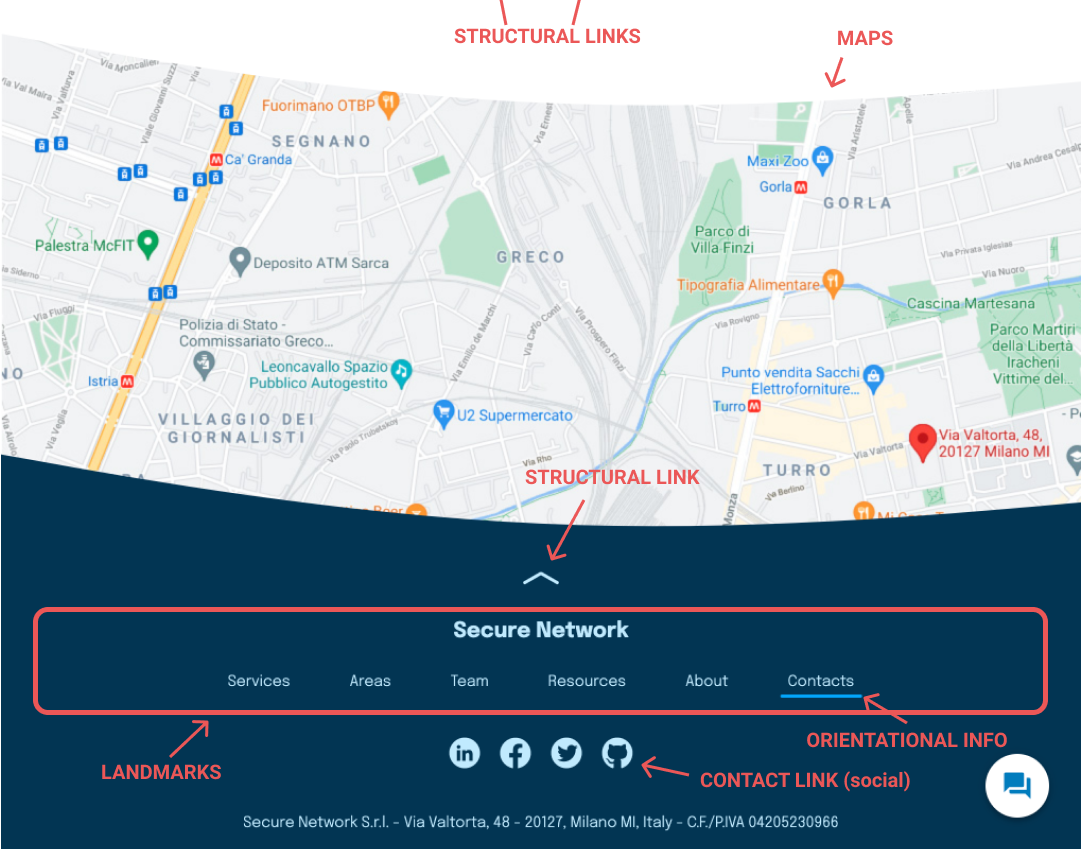
\includegraphics[width=0.45\textwidth]{high_fid_wireframes/contacts/3.png}
	\caption{Commented screenshots for the Contacts page.}
\end{figure}

\subsection{Kind of Topic: Area}

\begin{figure}[H]
	\centering
	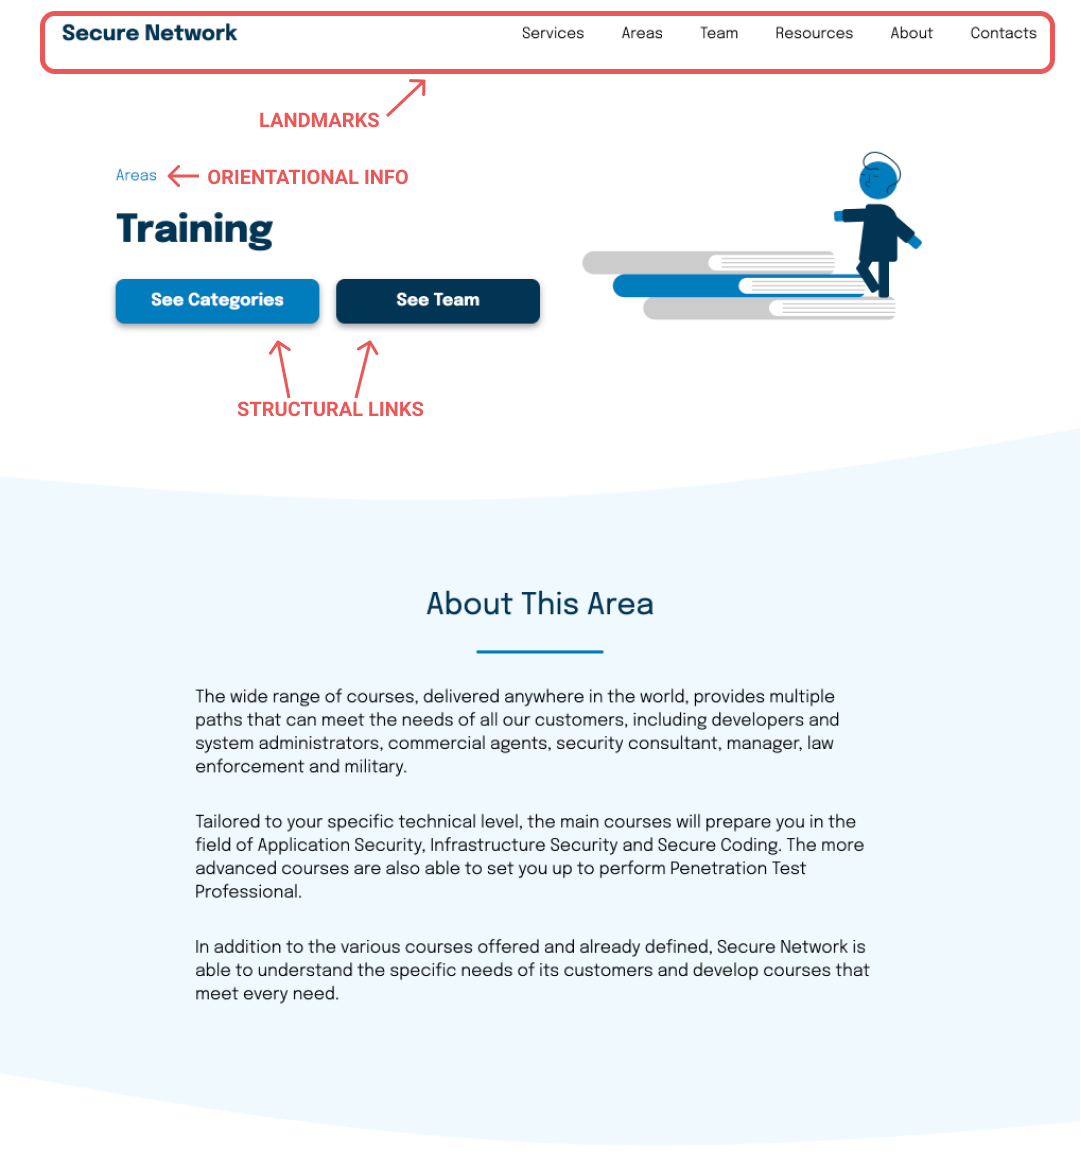
\includegraphics[width=0.45\textwidth]{high_fid_wireframes/area/1.png}
	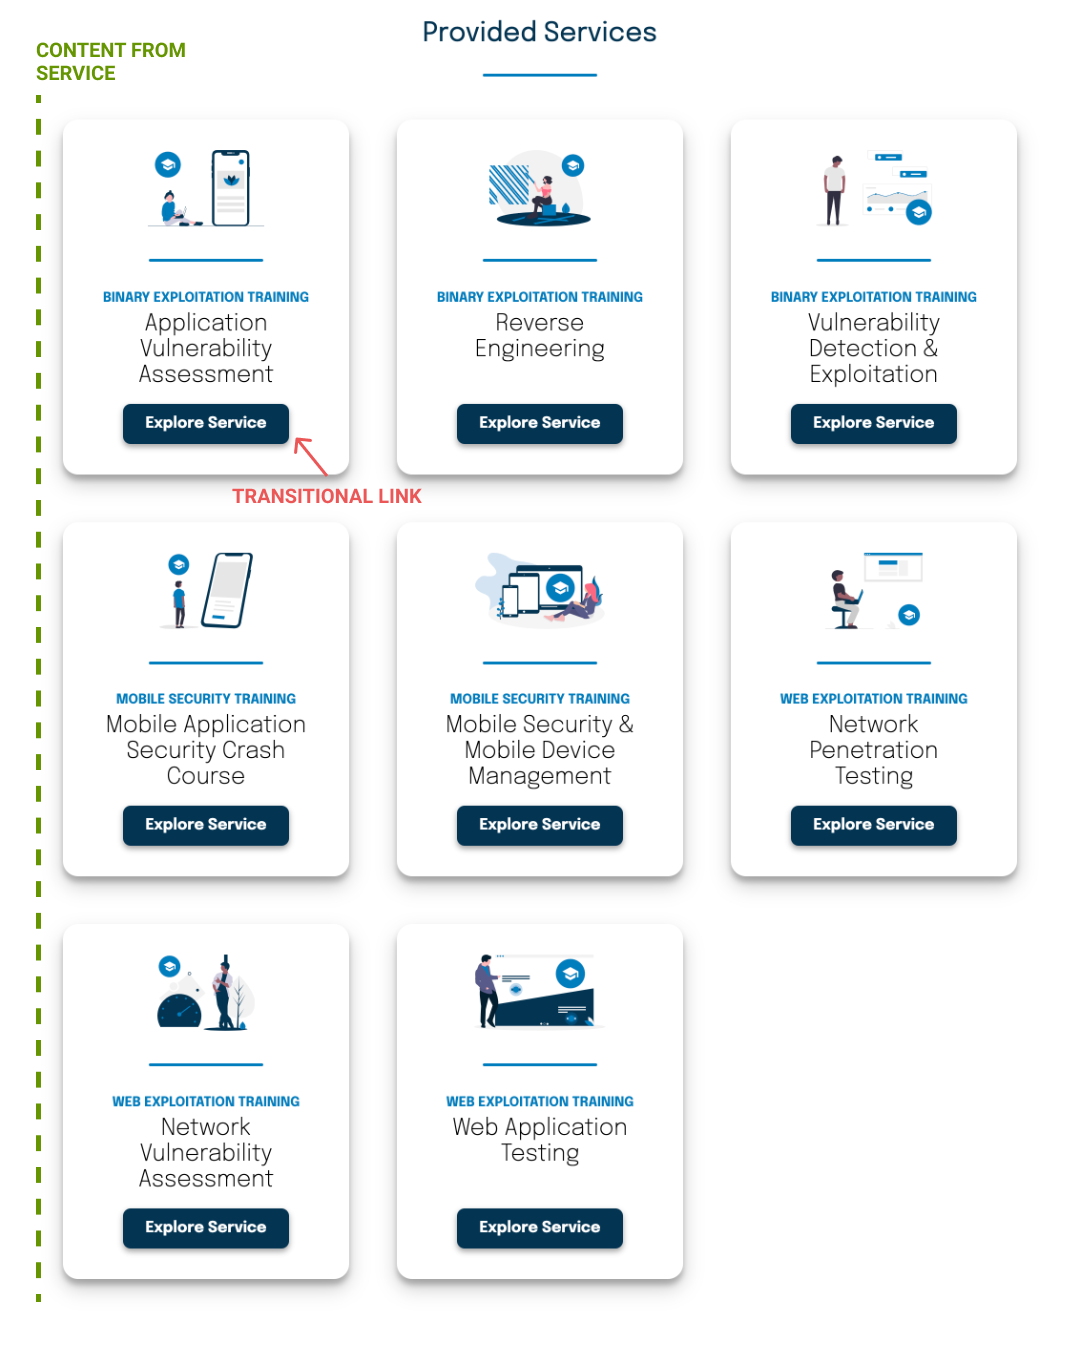
\includegraphics[width=0.45\textwidth]{high_fid_wireframes/area/2.png}
	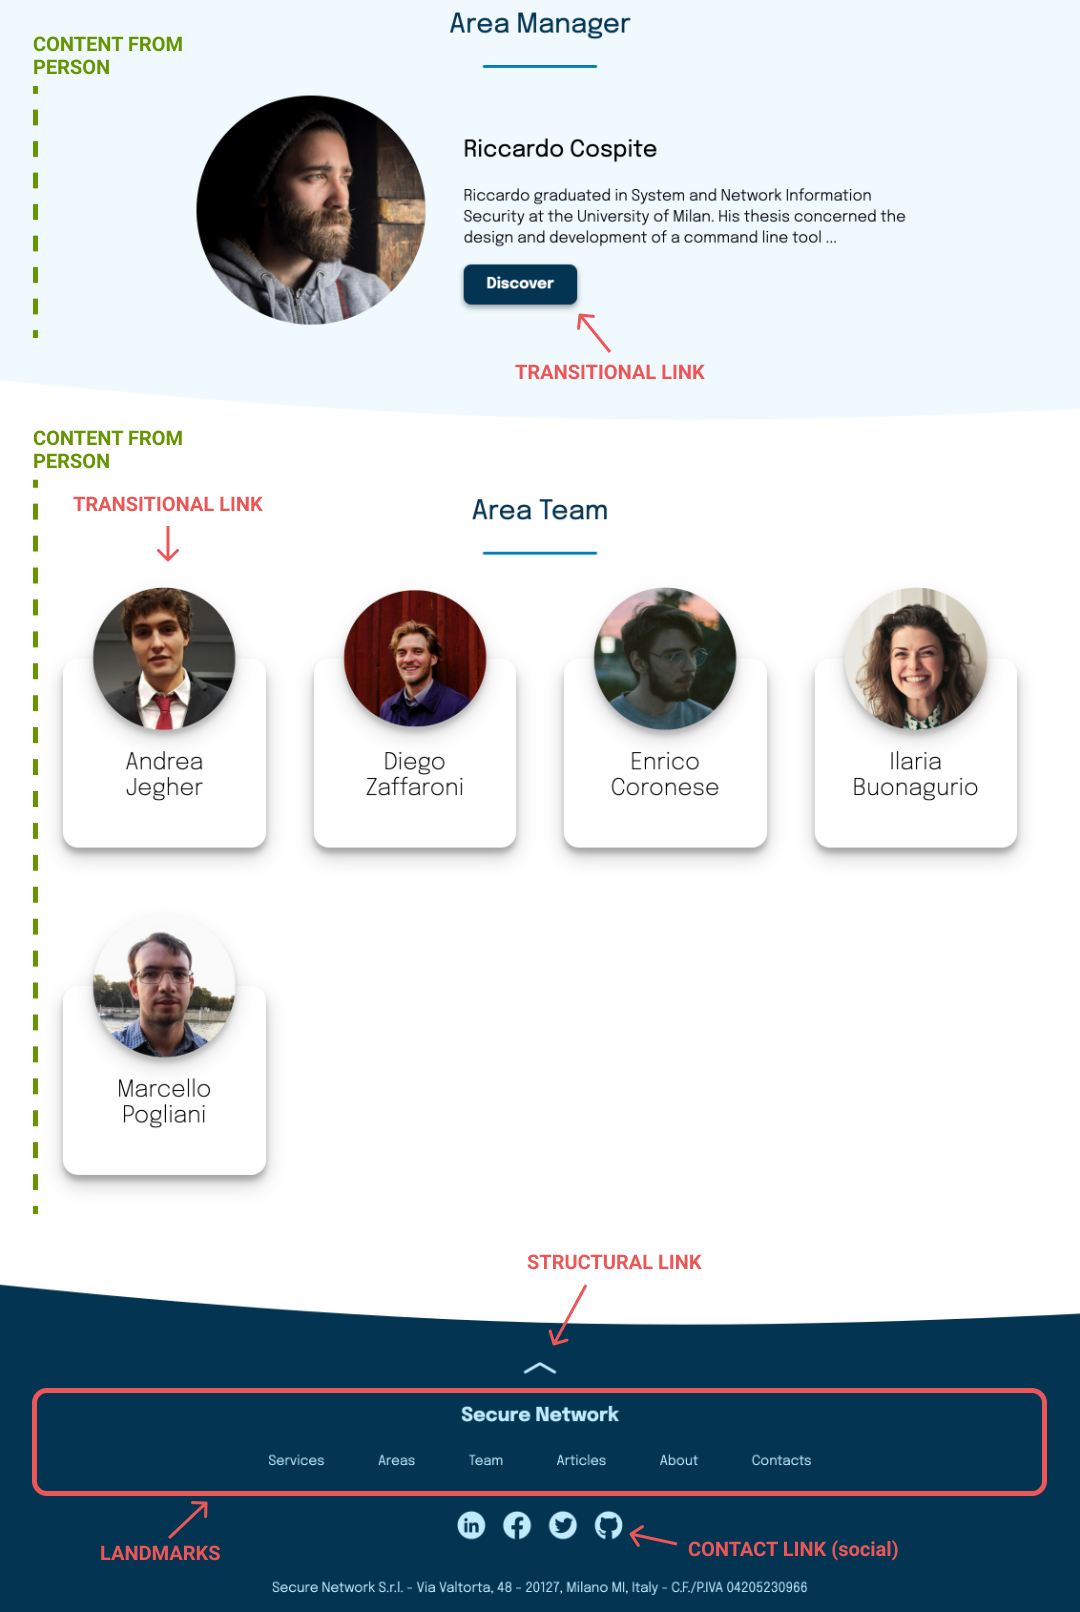
\includegraphics[width=0.45\textwidth]{high_fid_wireframes/area/3.png}
	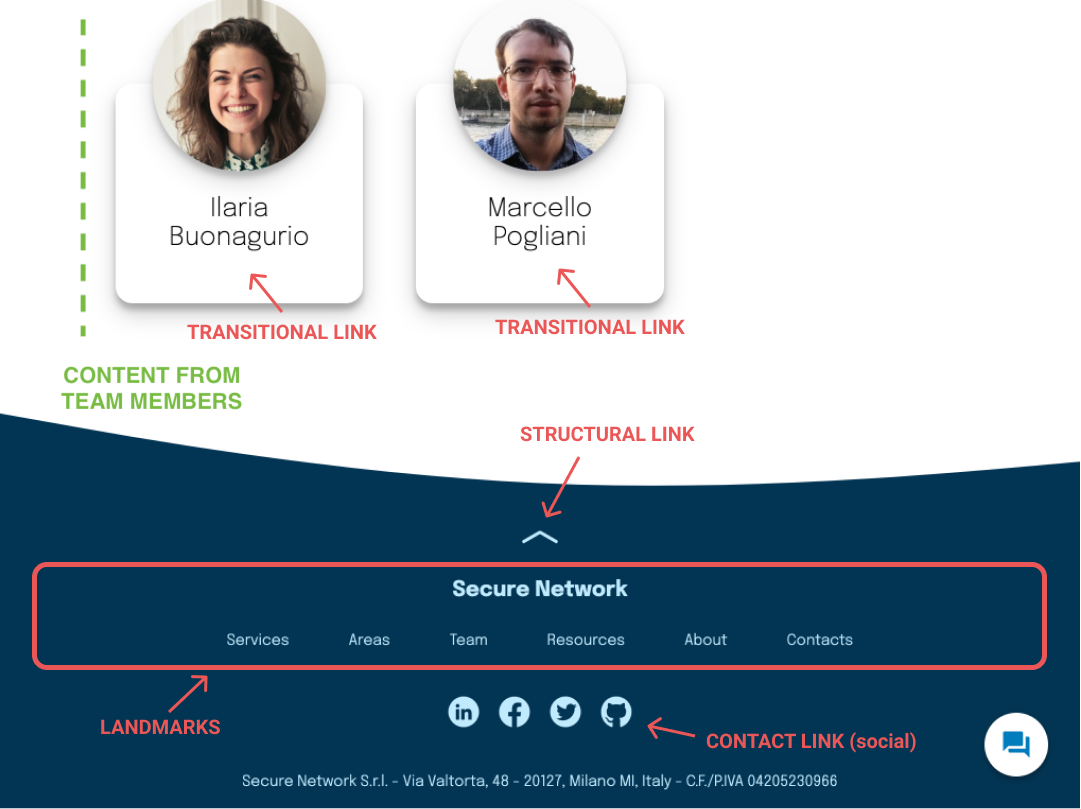
\includegraphics[width=0.45\textwidth]{high_fid_wireframes/area/4.png}
	\caption{Commented screenshots for the Area page.}
\end{figure}
\color{white}...\color{black}

\subsection{Kind of Topic: Person}

\begin{figure}[H]
	\centering
	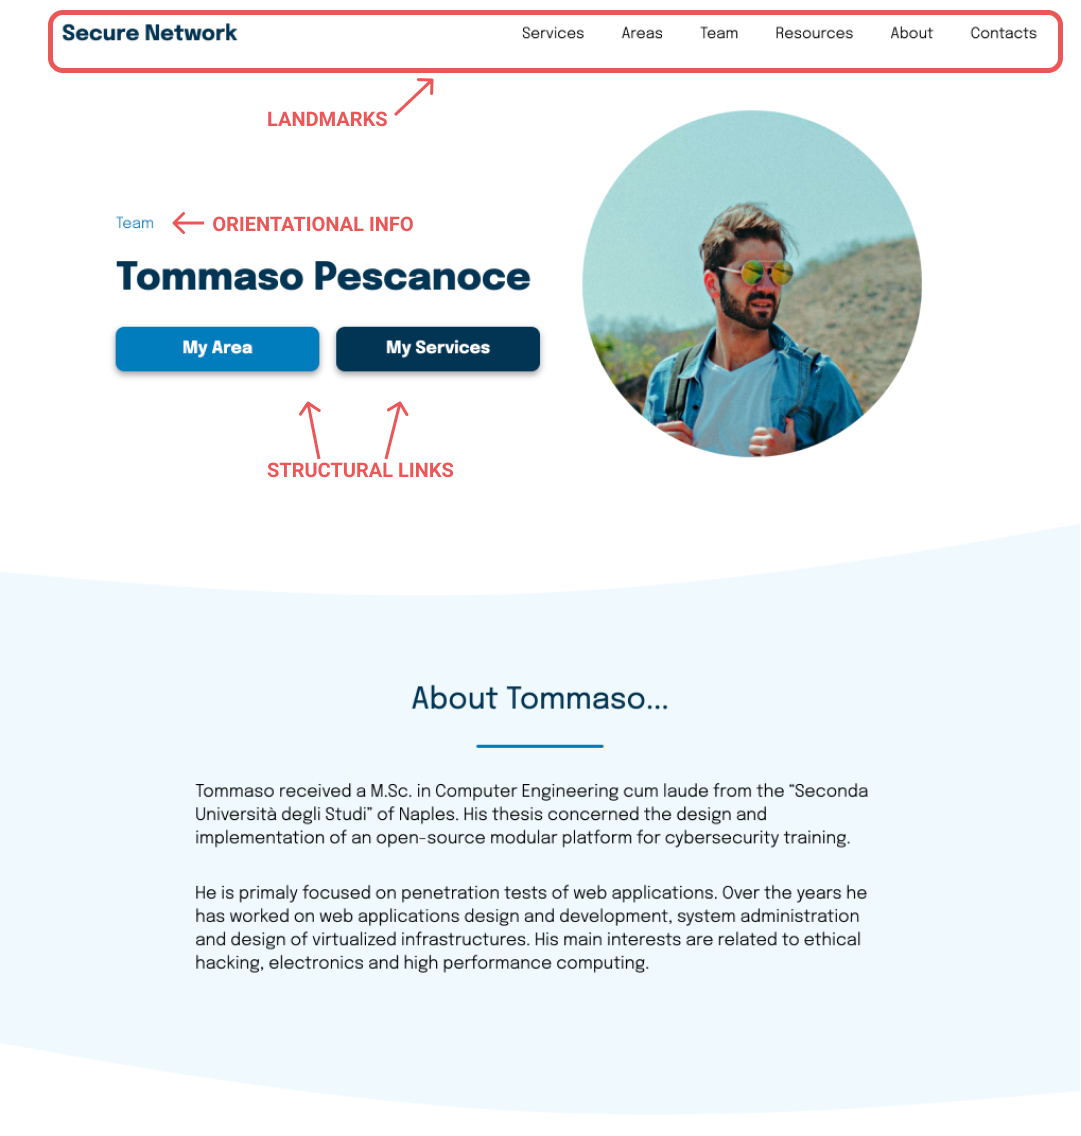
\includegraphics[width=0.45\textwidth]{high_fid_wireframes/person/1.png}
	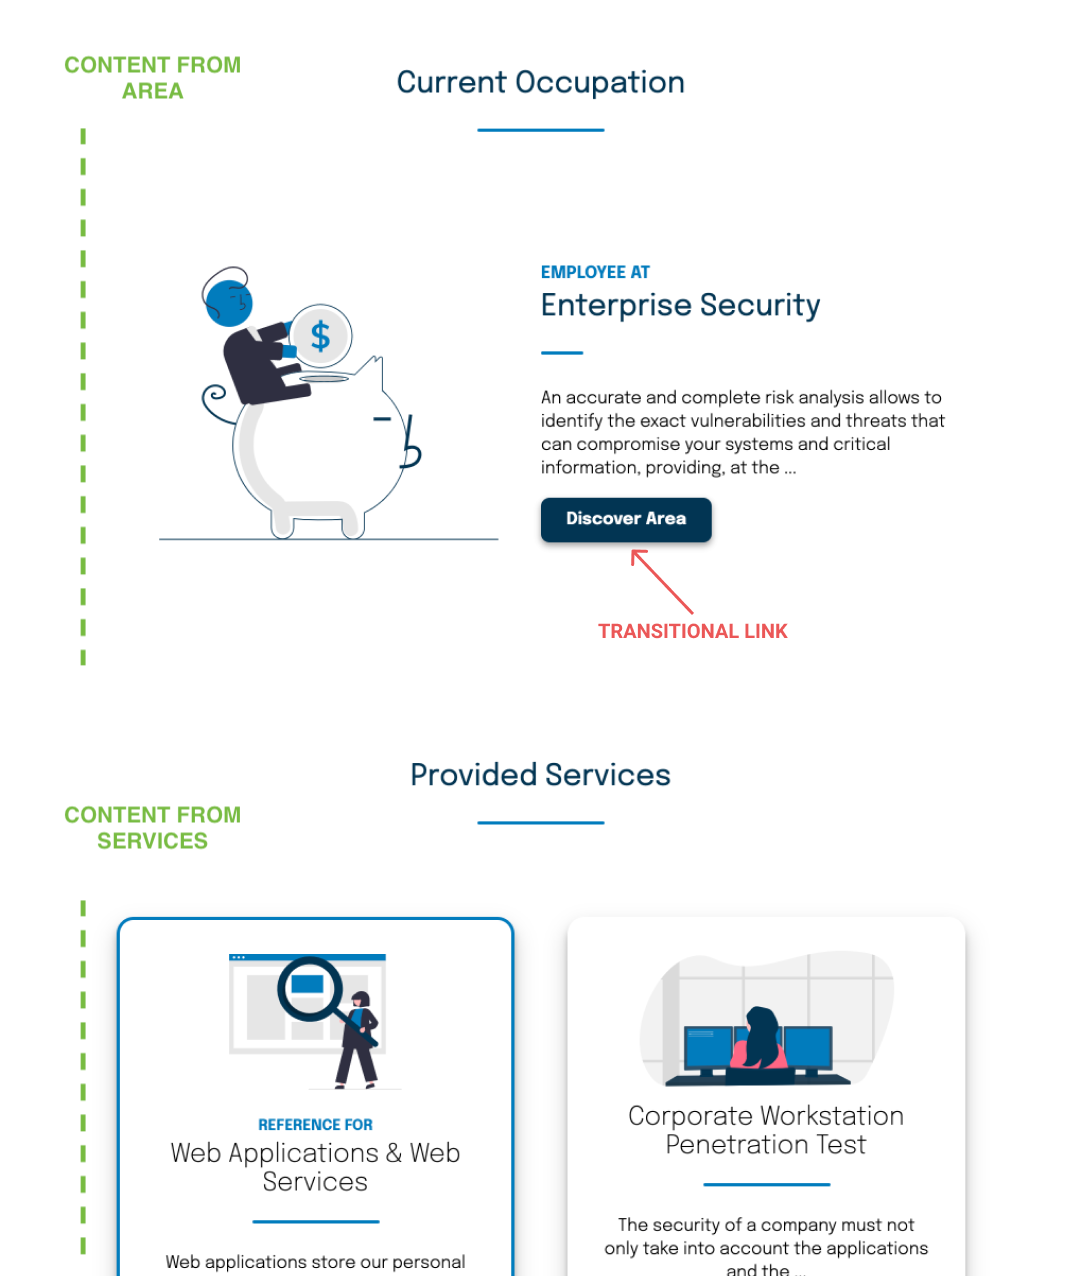
\includegraphics[width=0.45\textwidth]{high_fid_wireframes/person/2.png}
	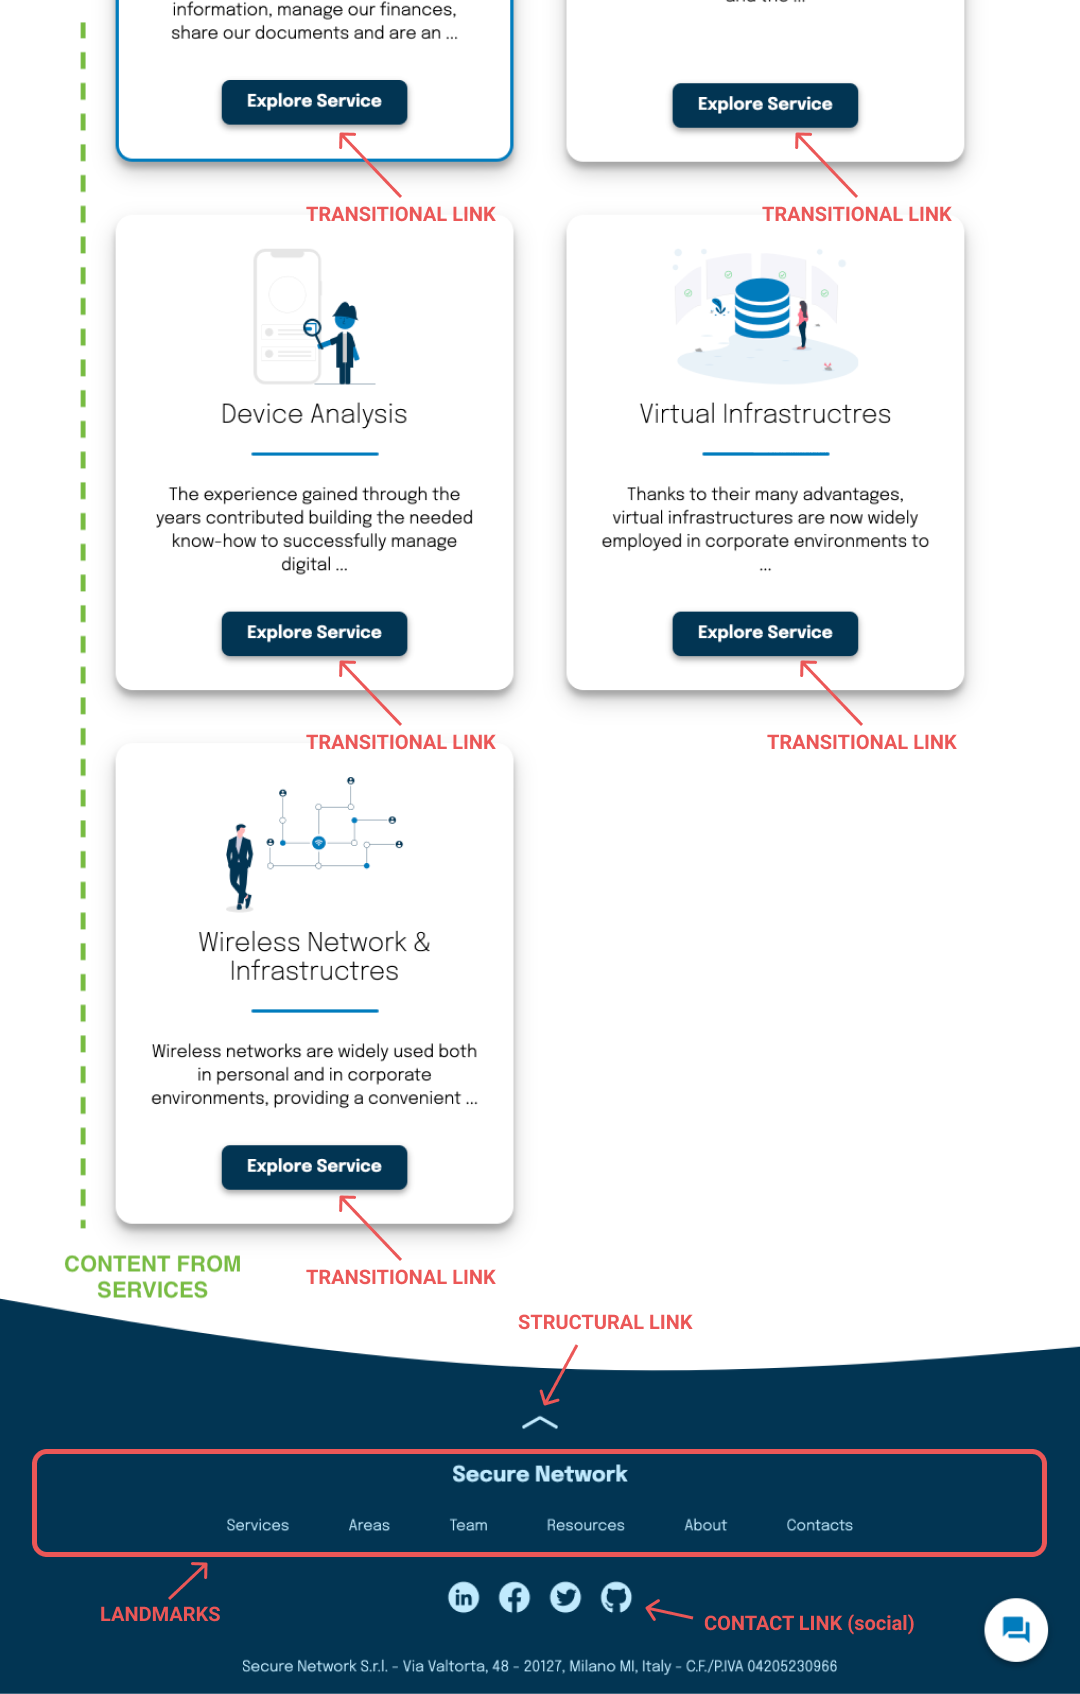
\includegraphics[width=0.45\textwidth]{high_fid_wireframes/person/3.png}
	\caption{Commented screenshots for the Person page.}
\end{figure}

\subsection{Kind of Topic: Service}

\begin{figure}[H]
	\centering
	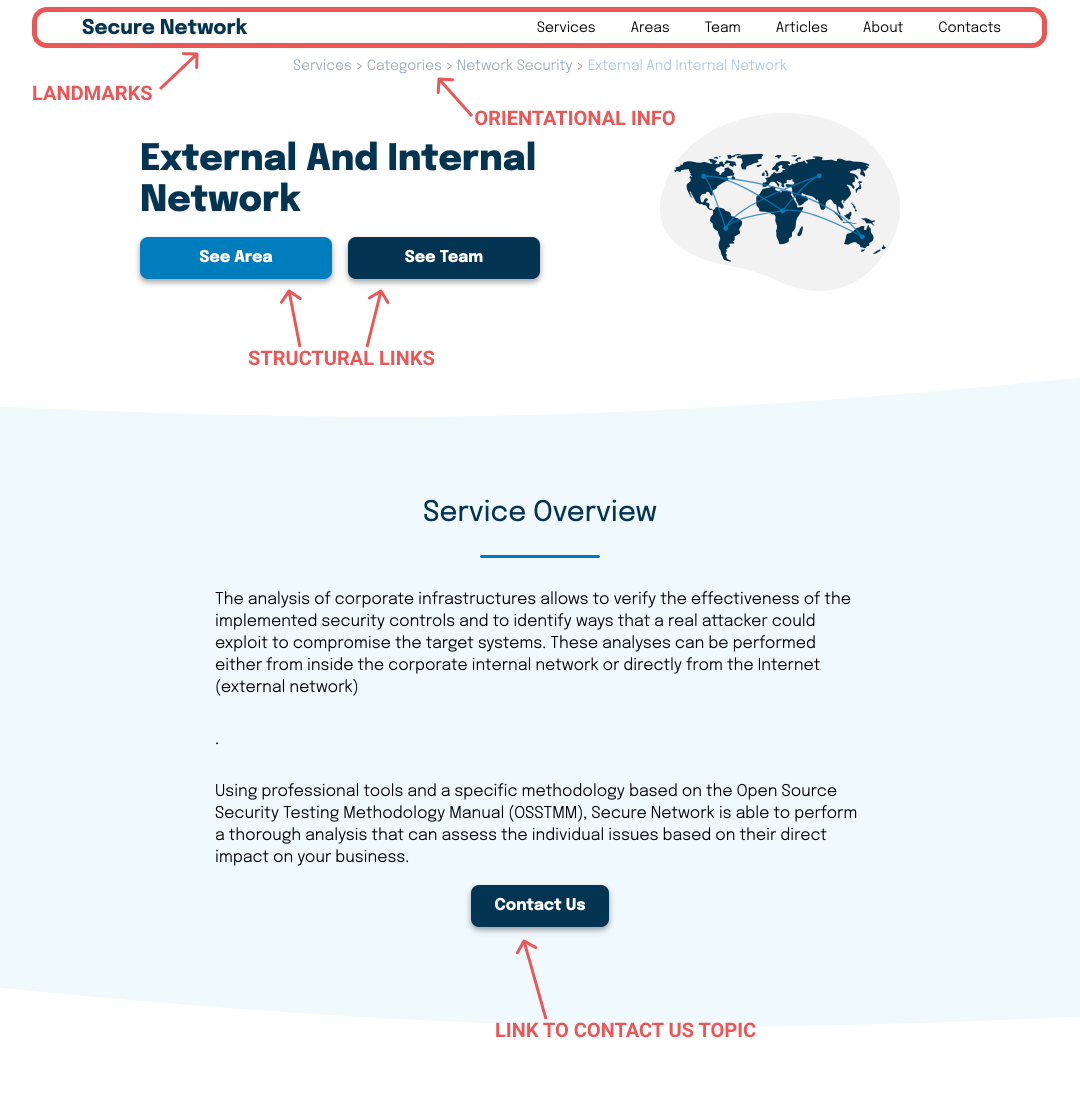
\includegraphics[width=0.45\textwidth]{high_fid_wireframes/service/1.png}
	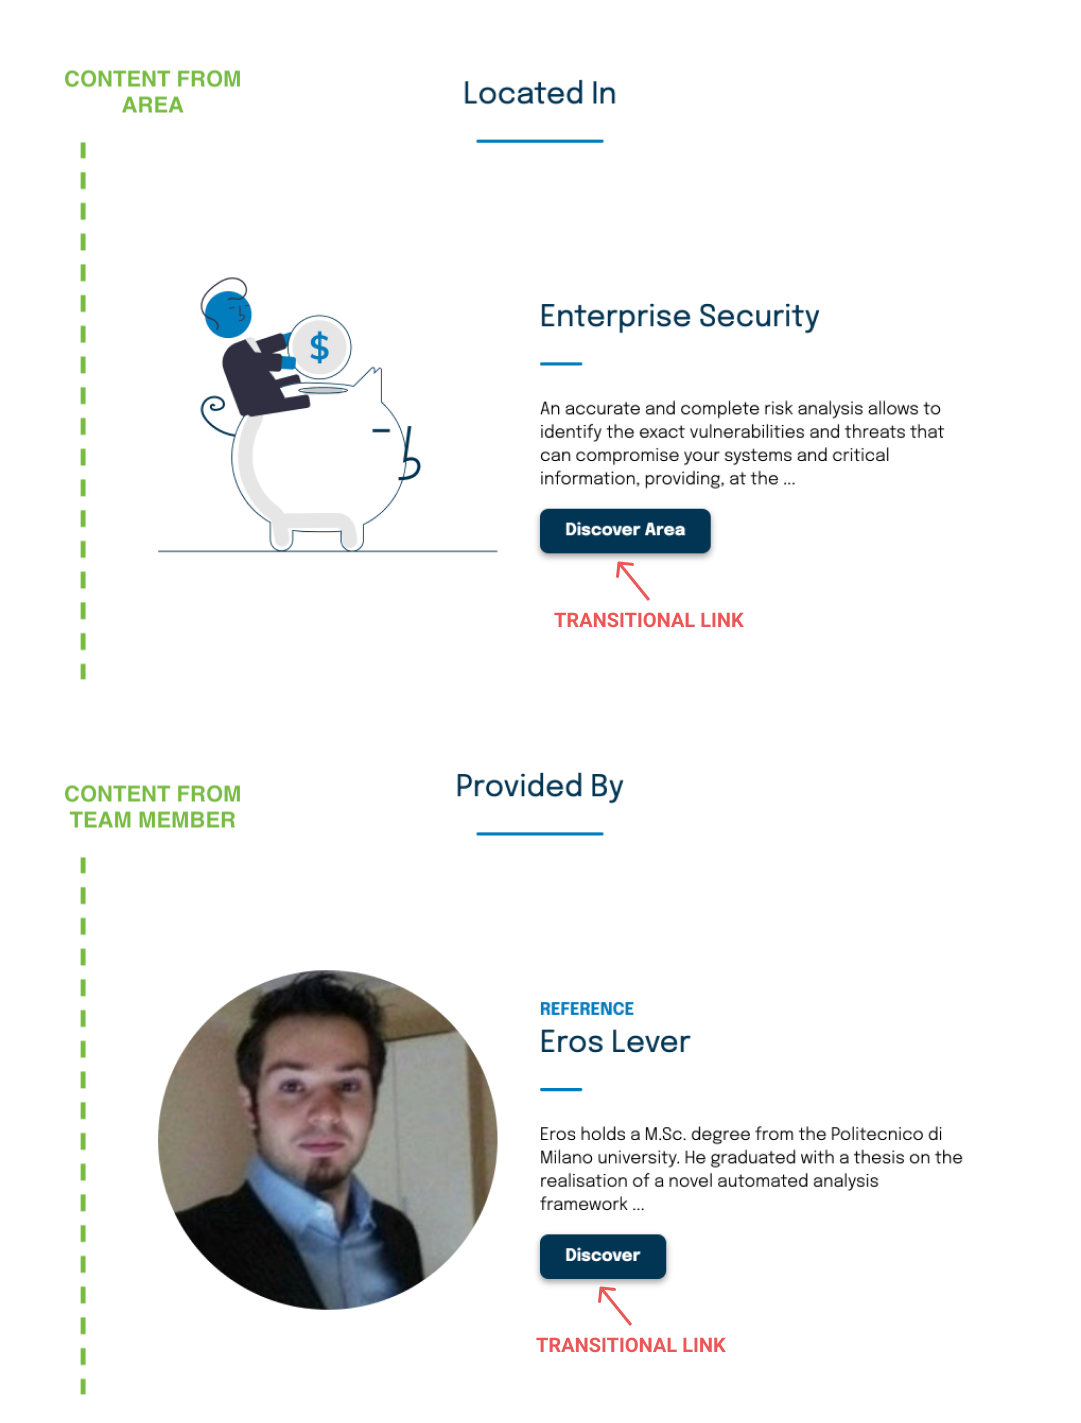
\includegraphics[width=0.45\textwidth]{high_fid_wireframes/service/2.png}
	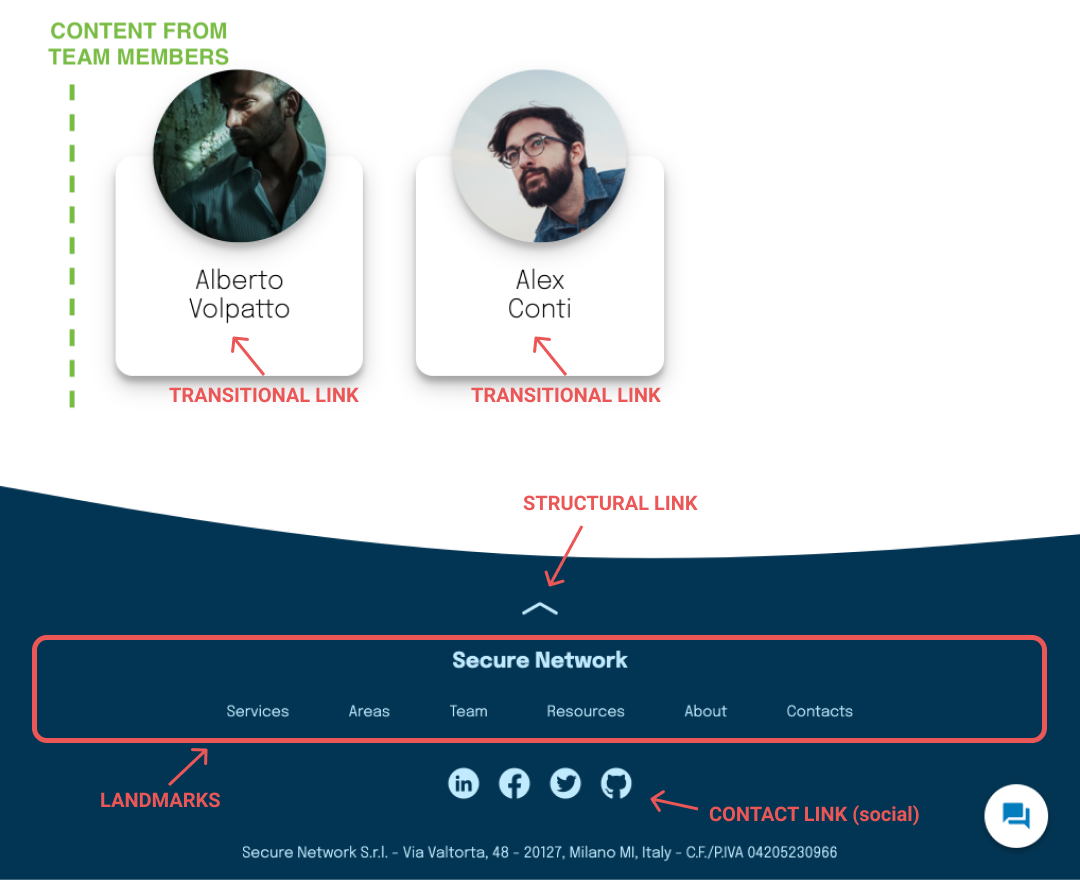
\includegraphics[width=0.45\textwidth]{high_fid_wireframes/service/3.png}
	\caption{Commented screenshots for the Service page.}
\end{figure}

\subsection{Kind of Topic: Resource}

\begin{figure}[H]
	\centering
	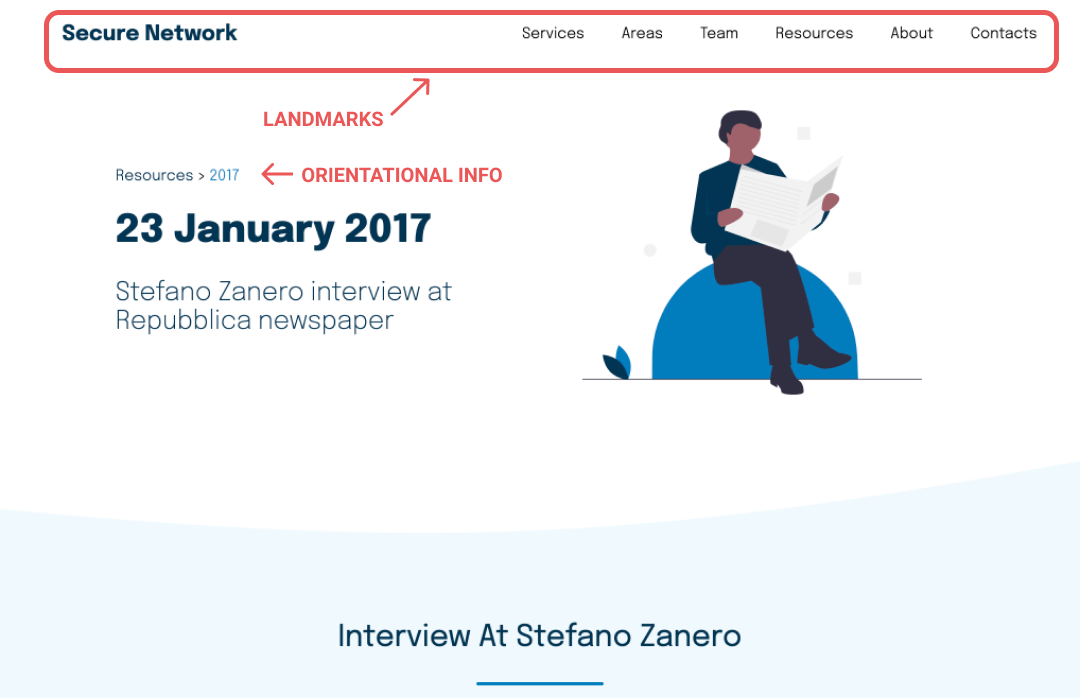
\includegraphics[width=0.45\textwidth]{high_fid_wireframes/resource/1.png}
	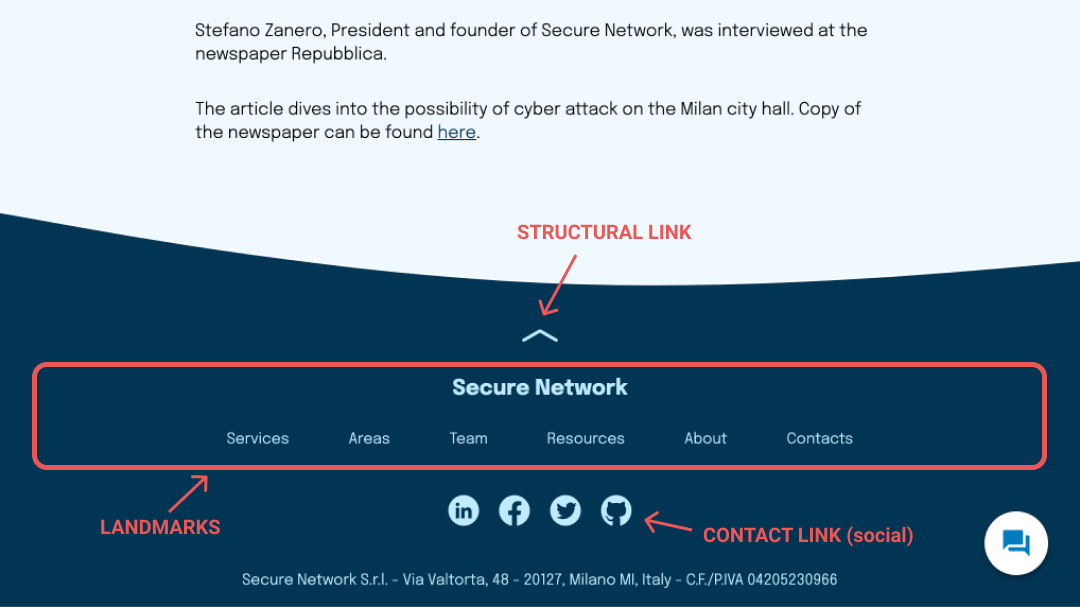
\includegraphics[width=0.45\textwidth]{high_fid_wireframes/resource/2.png}
	\caption{Commented screenshots for the Resources page.}
\end{figure}

\subsection{Group: Areas}

\begin{figure}[H]
	\centering
	\includegraphics[width=0.45\textwidth]{high_fid_wireframes/all_areas/1.png}
	\includegraphics[width=0.45\textwidth]{high_fid_wireframes/all_areas/2.png}
	\caption{Commented screenshots for the Areas page.}
\end{figure}

\subsection{Group: Team}

\begin{figure}[H]
	\centering
	\includegraphics[width=0.45\textwidth]{high_fid_wireframes/team/1.png}
	\includegraphics[width=0.45\textwidth]{high_fid_wireframes/team/2.png}
	\includegraphics[width=0.45\textwidth]{high_fid_wireframes/team/3.png}
	\caption{Commented screenshots for the Team page.}
\end{figure}

\subsection{Group: Resources}

\begin{figure}[H]
	\centering
	\includegraphics[width=0.45\textwidth]{high_fid_wireframes/all_resources/1.png}
	\includegraphics[width=0.45\textwidth]{high_fid_wireframes/all_resources/2.png}
	\caption{Commented screenshots for the Resources page.}
\end{figure}

\chapter{Interaction Scenarios}

\section{Scenario 1}
An attorney from the Milan prosecutor's office is looking for a company able to retrieve evidence from a device linked to a court case.\\
\noindent
She got the name of Secure Network and would like to find out if they can perform the job she is looking for and, in case, get a quote.
To do so, she connects to the company website.\\
\noindent
She directly goes to the \emph{Areas} page and, after reading the short abstracts, she chooses to visit the page of the \emph{Enterprise Security} area.
There, she clicks on \emph{See Categories} and examines the list that is shown to her.\\
\noindent
Among the options, she selects the \emph{Digital Forensics} category and, in the page that opens, she finds \emph{Forensics Acquisition} that seems to be exactly the service she needs.
After opening the page to confirm her assumptions, she browses to the \emph{Contacts} page to send them an email.

\begin{figure}[H]
	\centering
	\includegraphics[width=0.45\textwidth]{scenarios/1/1.png}
	\includegraphics[width=0.45\textwidth]{scenarios/1/2.png}
	\includegraphics[width=0.45\textwidth]{scenarios/1/3.png}
	\includegraphics[width=0.45\textwidth]{scenarios/1/4.png}
\end{figure}
\begin{figure}[H]
	\centering
	\includegraphics[width=0.45\textwidth]{scenarios/1/5.png}
	\includegraphics[width=0.45\textwidth]{scenarios/1/6.png}
	\includegraphics[width=0.45\textwidth]{scenarios/1/7.png}
	\caption{Screenshots describing interactive scenario 1.}
\end{figure}

\clearpage
\section{Scenario 2}
A recent graduate of the Politecnico is looking for his first job in the computer security field.
A few days ago, he attended a workshop given by Alvise Biffi in which he mentioned that the company he founded is hiring but unfortunately he does not remember the name.\\
\noindent
He thinks it is called Secure Network but, to be completely sure, he connects to their website and goes to the \emph{Team} page where he finds \emph{Alvise Biffi}.
After reading the founder's biography abstract and decides to visit his page to have a complete reading. 
\\
\noindent
After that, he goes back to the \emph{Team} page (using the breadcrumbs on top of the page) to give another look to the employee list and there he finds the \emph{We are hiring} title and clicks on the \emph{Contact Us} button.

\begin{figure}[H]
	\centering
	\includegraphics[width=0.45\textwidth]{scenarios/2/1.png}
	\includegraphics[width=0.45\textwidth]{scenarios/2/2.png}
	\includegraphics[width=0.45\textwidth]{scenarios/2/3.png}
	\includegraphics[width=0.45\textwidth]{scenarios/2/4.png}
	\includegraphics[width=0.45\textwidth]{scenarios/2/5.png}
	\caption{Screenshots describing interactive scenario 2.}
\end{figure}

\clearpage
\section{Scenario 3}
During a conference, an enterpreneur came in contact with this security company from Milan that is called Secure Network.
He is impressed with what he heared about them and would like to discover what they do more in depth.
\\
\noindent
After connecting to the website, he browses the \emph{Home} page and reads the description of the company. 
He decides to click the \emph{About Us} button and in that page he discovers more about their history.
\\
\noindent
There, he finds a section where the company gives some reason why cybersecurity matters and decides to give a look to the \emph{Services} they offer.
He only wants to have an overview, so he decides to click on the \emph{Group by Category} button in order to have a look at that list.

\begin{figure}[H]
	\centering
	\includegraphics[width=0.45\textwidth]{scenarios/3/1.png}
	\includegraphics[width=0.45\textwidth]{scenarios/3/2.png}
	\includegraphics[width=0.45\textwidth]{scenarios/3/3.png}
	\includegraphics[width=0.45\textwidth]{scenarios/3/4.png}
	\caption{Screenshots describing interactive scenario 3.}
\end{figure}

\clearpage
\section{Scenario 4}
During a lecture of his course of Computer Security at Politecnico, professor Stefano Zanero mentioned an interview with him published in 2017.
One of his students would really like to read it so she visits to the website of his company, Secure Network, as he told her to do.
\\
\noindent
Right on the \emph{Home} page, she finds some of the latest news and she spots one about his professor that she wants to read.
After reading that article, she goes back to the \emph{Resources} page using the breadcrumbs on top and she selects the year \emph{2017}.
\\
\noindent
Once on the year page, she filters the resources to see only the news and then she finds the interview that she was looking for.

\begin{figure}[H]
	\centering
	\includegraphics[width=0.45\textwidth]{scenarios/4/1.png}
	\includegraphics[width=0.45\textwidth]{scenarios/4/2.png}
	\includegraphics[width=0.45\textwidth]{scenarios/4/3.png}
	\includegraphics[width=0.45\textwidth]{scenarios/4/4.png}
	\includegraphics[width=0.45\textwidth]{scenarios/4/5.png}
	\caption{Screenshots describing interactive scenario 4.}
\end{figure}

\chapter{DB Design}
In this last chapter we report the structure of the database designed 
to support the website and manage the information contained in it. 
We started with the conceptual design, by which is possible to identify
the first layer of abstraction of our data. It has been moded with the 
\emph{Entity-Relationship diagram}.\\
\begin{figure}[H]
	\centering
	\includegraphics[width=0.95\textwidth]{ER_model.pdf}
	\caption{ER Diagram}
\end{figure}
\noindent
Then we proceed with the logic design, which allow to better describe the
\emph{E-R Model}. Some additional tables have been identified to better 
support the implementation.
\clearpage
\begin{itemize}
	\item \textbf{Area}. An \emph{Area} is identified by an \texttt{id}, 
	has a \texttt{name}, a \texttt{text} description, a string path to the image, 
	\texttt{img}, and a \texttt{path} to reach the specific page. 
	\item \textbf{Person}. A \emph{Person} is identified by an \texttt{id}, 
	has a \texttt{name}, a \texttt{surname}, a \texttt{text} description, a 
	string path to the image, \texttt{img}, a \texttt{path} to reach the specific page.
	In addition, the relation called \emph{Assignment}, among \emph{Person} and \emph{Area}, has
	been merged within the first table, resulting in the addition of two fiels: the 
	\texttt{area\_id} as foreign key and the \texttt{role} of the person within the area.
	Each \emph{Person} is assigned to exactly one \emph{Area}, whereas in each \emph{Area} several
	\emph{People} are assigned.
	\item \textbf{Service\_Category}. This tables was born due to normalization purposes. 
	It would have been redundant adding for each \emph{Service} information about the complex 
	attribute \emph{Category}. To avoid replication, we decided to perform this normalization 
	procedure. A \emph{Service\_Category} is identified by an \texttt{id}, 
	has a \texttt{name}, a \texttt{text} description, a string path to the image, 
	\texttt{img}, and a \texttt{path} to reach the specific page. 
	\item \textbf{Service}. A \emph{Service} is identified by an \texttt{id}, 
	has a \texttt{name}, a \texttt{text} description, a string path to the image, \texttt{img}, 
	a \texttt{path} to reach the specific page.
	The \texttt{category\_id} is the foreign key, used to support the normalization process 
	described in the previous table. 
	Each \emph{Service} is mapped with exactly one \emph{Service\_Category}, whereas each 
	\emph{Service\_Category} is mapped with several \emph{Services}.
	In addition, the relation called \emph{Offer}, among 
	\emph{Service} and \emph{Area}, has	been merged within the first table, resulting in 
	the addition of the fiel \texttt{area\_id} as foreign key.
	Each \emph{Service} is offered by exactly one \emph{Area}, whereas each \emph{Area} offers 
	several \emph{Services}.
	\item \textbf{Person\_Service}. This tables was born to support the \emph{N-N} relation, 
	\emph{Provide}, among \emph{Person} and \emph{Service}. A \emph{Person\_Service} is 
	identified by an autoincremental \texttt{id} and presents a boolean field, \texttt{isReference}, 
	which states whether or not the \emph{Person}, identified by the foreign key \texttt{person\_id}, 
	is the reference for the \emph{Service}, identified by the foreign key \texttt{service\_id}.
	\item \textbf{Resource}. A \emph{Resource} is identified by an \texttt{id}, has a 
	\texttt{type}, a \texttt{name}, a \texttt{date}, a \texttt{text} description, a \texttt{subtitle} 
	a string path to the \texttt{icon}, and a \texttt{path} to reach the specific page. 
\end{itemize}


\begin{figure}[H]
	\centering
	\includegraphics[width=0.95\textwidth]{ER-Logic-Tables.pdf}
	\caption{Relational Tables}
\end{figure}


\listoffigures
\end{document}